\chapter{RRT Flight Corridors}
\label{ch:rrt_flight_corridors}

In subsection \ref{sec:vtol path planning}, several B-Spline paths were created for the quadplane eVTOL to follow. 
These paths were relatively simple because it was assumed that no obstacles were present in the environment. 
Obstacles are present in many cases, and this assumption becomes invalidated. 
An example of this is an urban environment with obstacles including buildings, wires, poles, vehicles, and people. 
The 2D eVTOL controller developed in section \ref{ch:VTOL} requires a B-Spline input to function. 
These constraints make it necessary to develop an algorithm that generates a B-Spline trajectory while simultaneously avoiding obstacles.

A great deal of literature exists on obstacle-avoiding path generation algorithms. 
In \cite{david_bspline}, much of the work that is foundational to this paper was developed.
Chapter 4 of that paper focuses on trajectory generation algorithms with obstacle avoidance and boundary constraints in both 2D and 3D. 
One problem addressed in the paper is path generation with obstacle avoidance for circular obstacles. 
The algorithm optimizes the path to minimize distance without intersecting circular or spherical obstacles in the 2D and 3D cases respectively.


\begin{figure}[htbp]
    \centering
    \begin{minipage}{0.48\textwidth}
        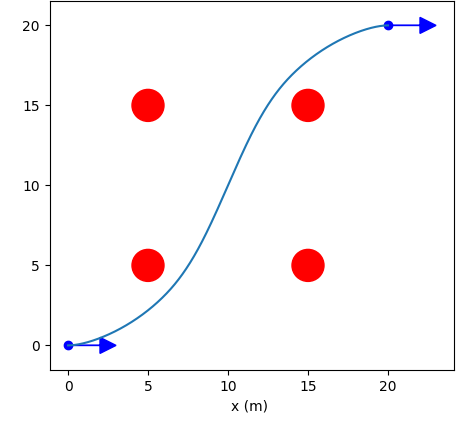
\includegraphics[width=\textwidth]{figs/chap1/david_2x2.png}
        \vspace{1em}
        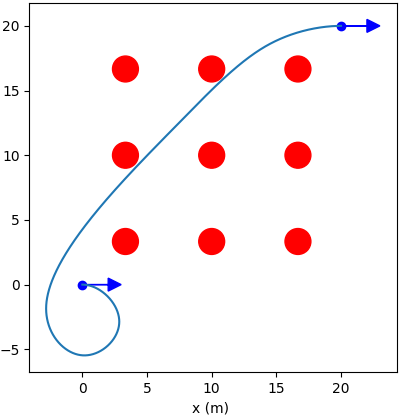
\includegraphics[width=\textwidth]{figs/chap1/david_3x3.png}
    \end{minipage}
    \hfill
    \begin{minipage}{0.48\textwidth}
        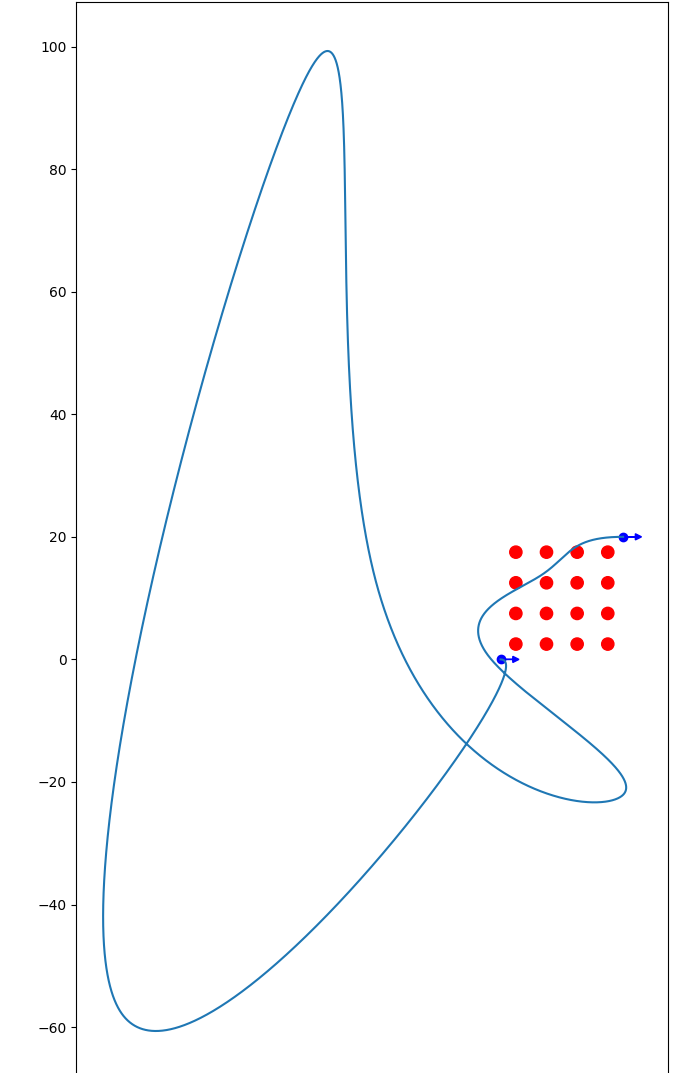
\includegraphics[width=\textwidth,height=\textheight,keepaspectratio]{figs/chap1/david_4x4.png}
    \end{minipage}
    \caption{Three examples of obstacle fields are presented. The 2x2 and 3x3 grids run fairly well. The algorithm breaks down on the 4x4 grid; it does not find a good initialization point.}
    \label{fig:davidObstacleComparison}
\end{figure}

The paper also uses safe flight corridors as constraints for the trajectory. 
Safe flight corridors are rectangles or rectangular prisms, which the flight path must completely remain inside. 
However, the algorithms presented in that paper do not search through obstacles paths.
Instead, they begin with an initial guess and optimize around obstacles and within safe flight corridors using that guess.

A B-Spline trajectory generation algorithm is developed in this section that plans safe paths for aircraft to follow through obstacle fields. 
A variant of the RRT algorithm is developed to place overlapping rectangular safe flight corridors through the field. 
Within these overlapping safe flight corridors, a flight path is generated using B-Splines. 
These B-Splines are created by adjusting control points so that the path always remains within the boundaries.

\section{Rapidly Exploring Random Trees (RRT)}

Rapidly Exploring Random Trees (RRT) is an algorithm that finds a path between two points through an obstacle field. 
The algorithm was first introduced in \cite{Lavalle_rrt} in 1999. 
The RRT algorithm generates a tree of nodes connected by lines, where none of the lines or nodes intersect obstacles.
The algorithm begins with the starting point as the first node. 
New nodes are added to the tree by randomly generating a position within the field. 
A line is drawn from that randomized position to the closest node on the existing tree, which is the starting point for the algorithm's first iteration. 
At a given point along that line, at distance $d$ away from the nearest node, a new candidate node is made. 
If the candidate node, and the line connecting to its parent node, does not intersect any obstacle, it is added to the tree as a new branch
However, if there is an intersection, the candidate node is discarded and the process is repeated with another randomized node. 
This process of randomly generating nodes and adding them to the existing tree is shown in Fig. \ref{fig:new node diagram}. 
This process is repeated until a valid path is found from the starting node to a specified finish node.
An example diagram of a tree with a valid path is shown in Fig. \ref{fig:straight line RRT}.


\begin{figure}
    \centering
    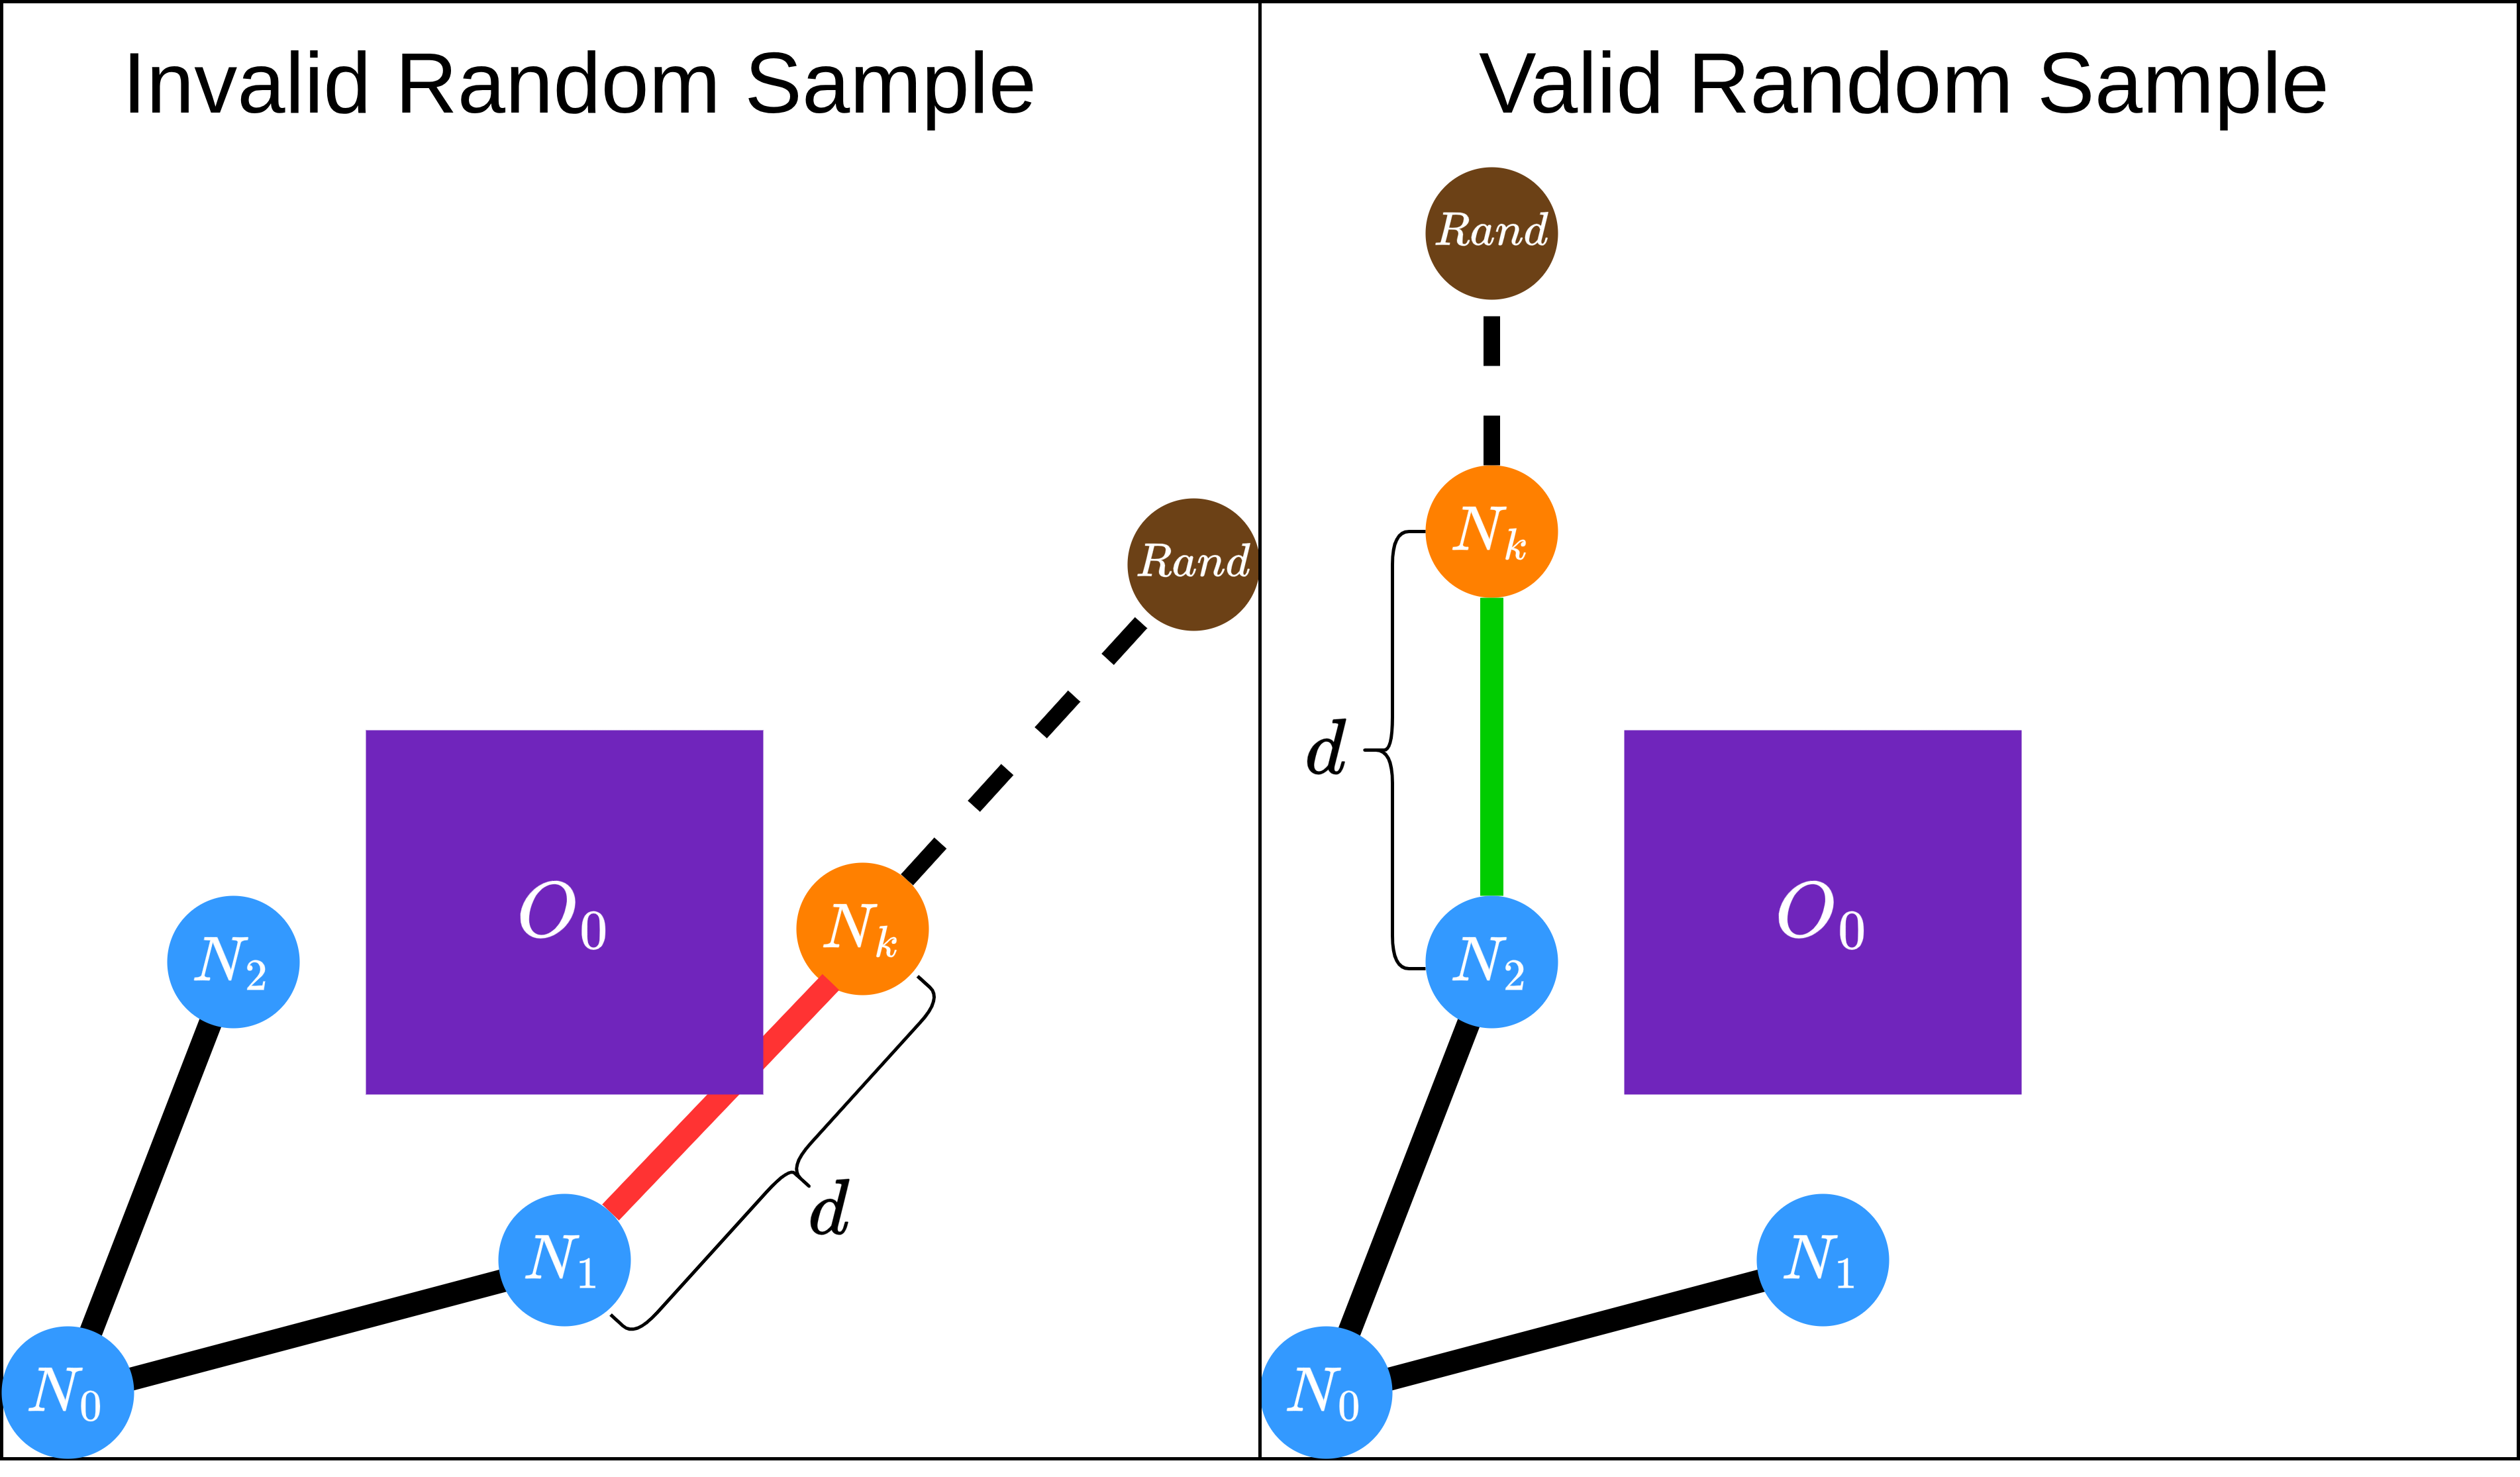
\includegraphics[width=0.95\linewidth]{figs/chap4/New Node Diagram.drawio.png}
    \caption{Point to point RRT expansion process. Two configurations are shown. 
            A random point $Rand$ is selected in the configuration space, a line is drawn between $Rand$ and the nearest existing node $N_i$. 
            A new candidate node $N_k$ is placed a distance $d$ from $N_i$. 
            If the line from $N_i$ to $N_k$ is not obstructed, it is added. 
            Otherwise, it is discarded, as in the invalid case.}
    \label{fig:new node diagram}
\end{figure}

\begin{figure}
    \centering
    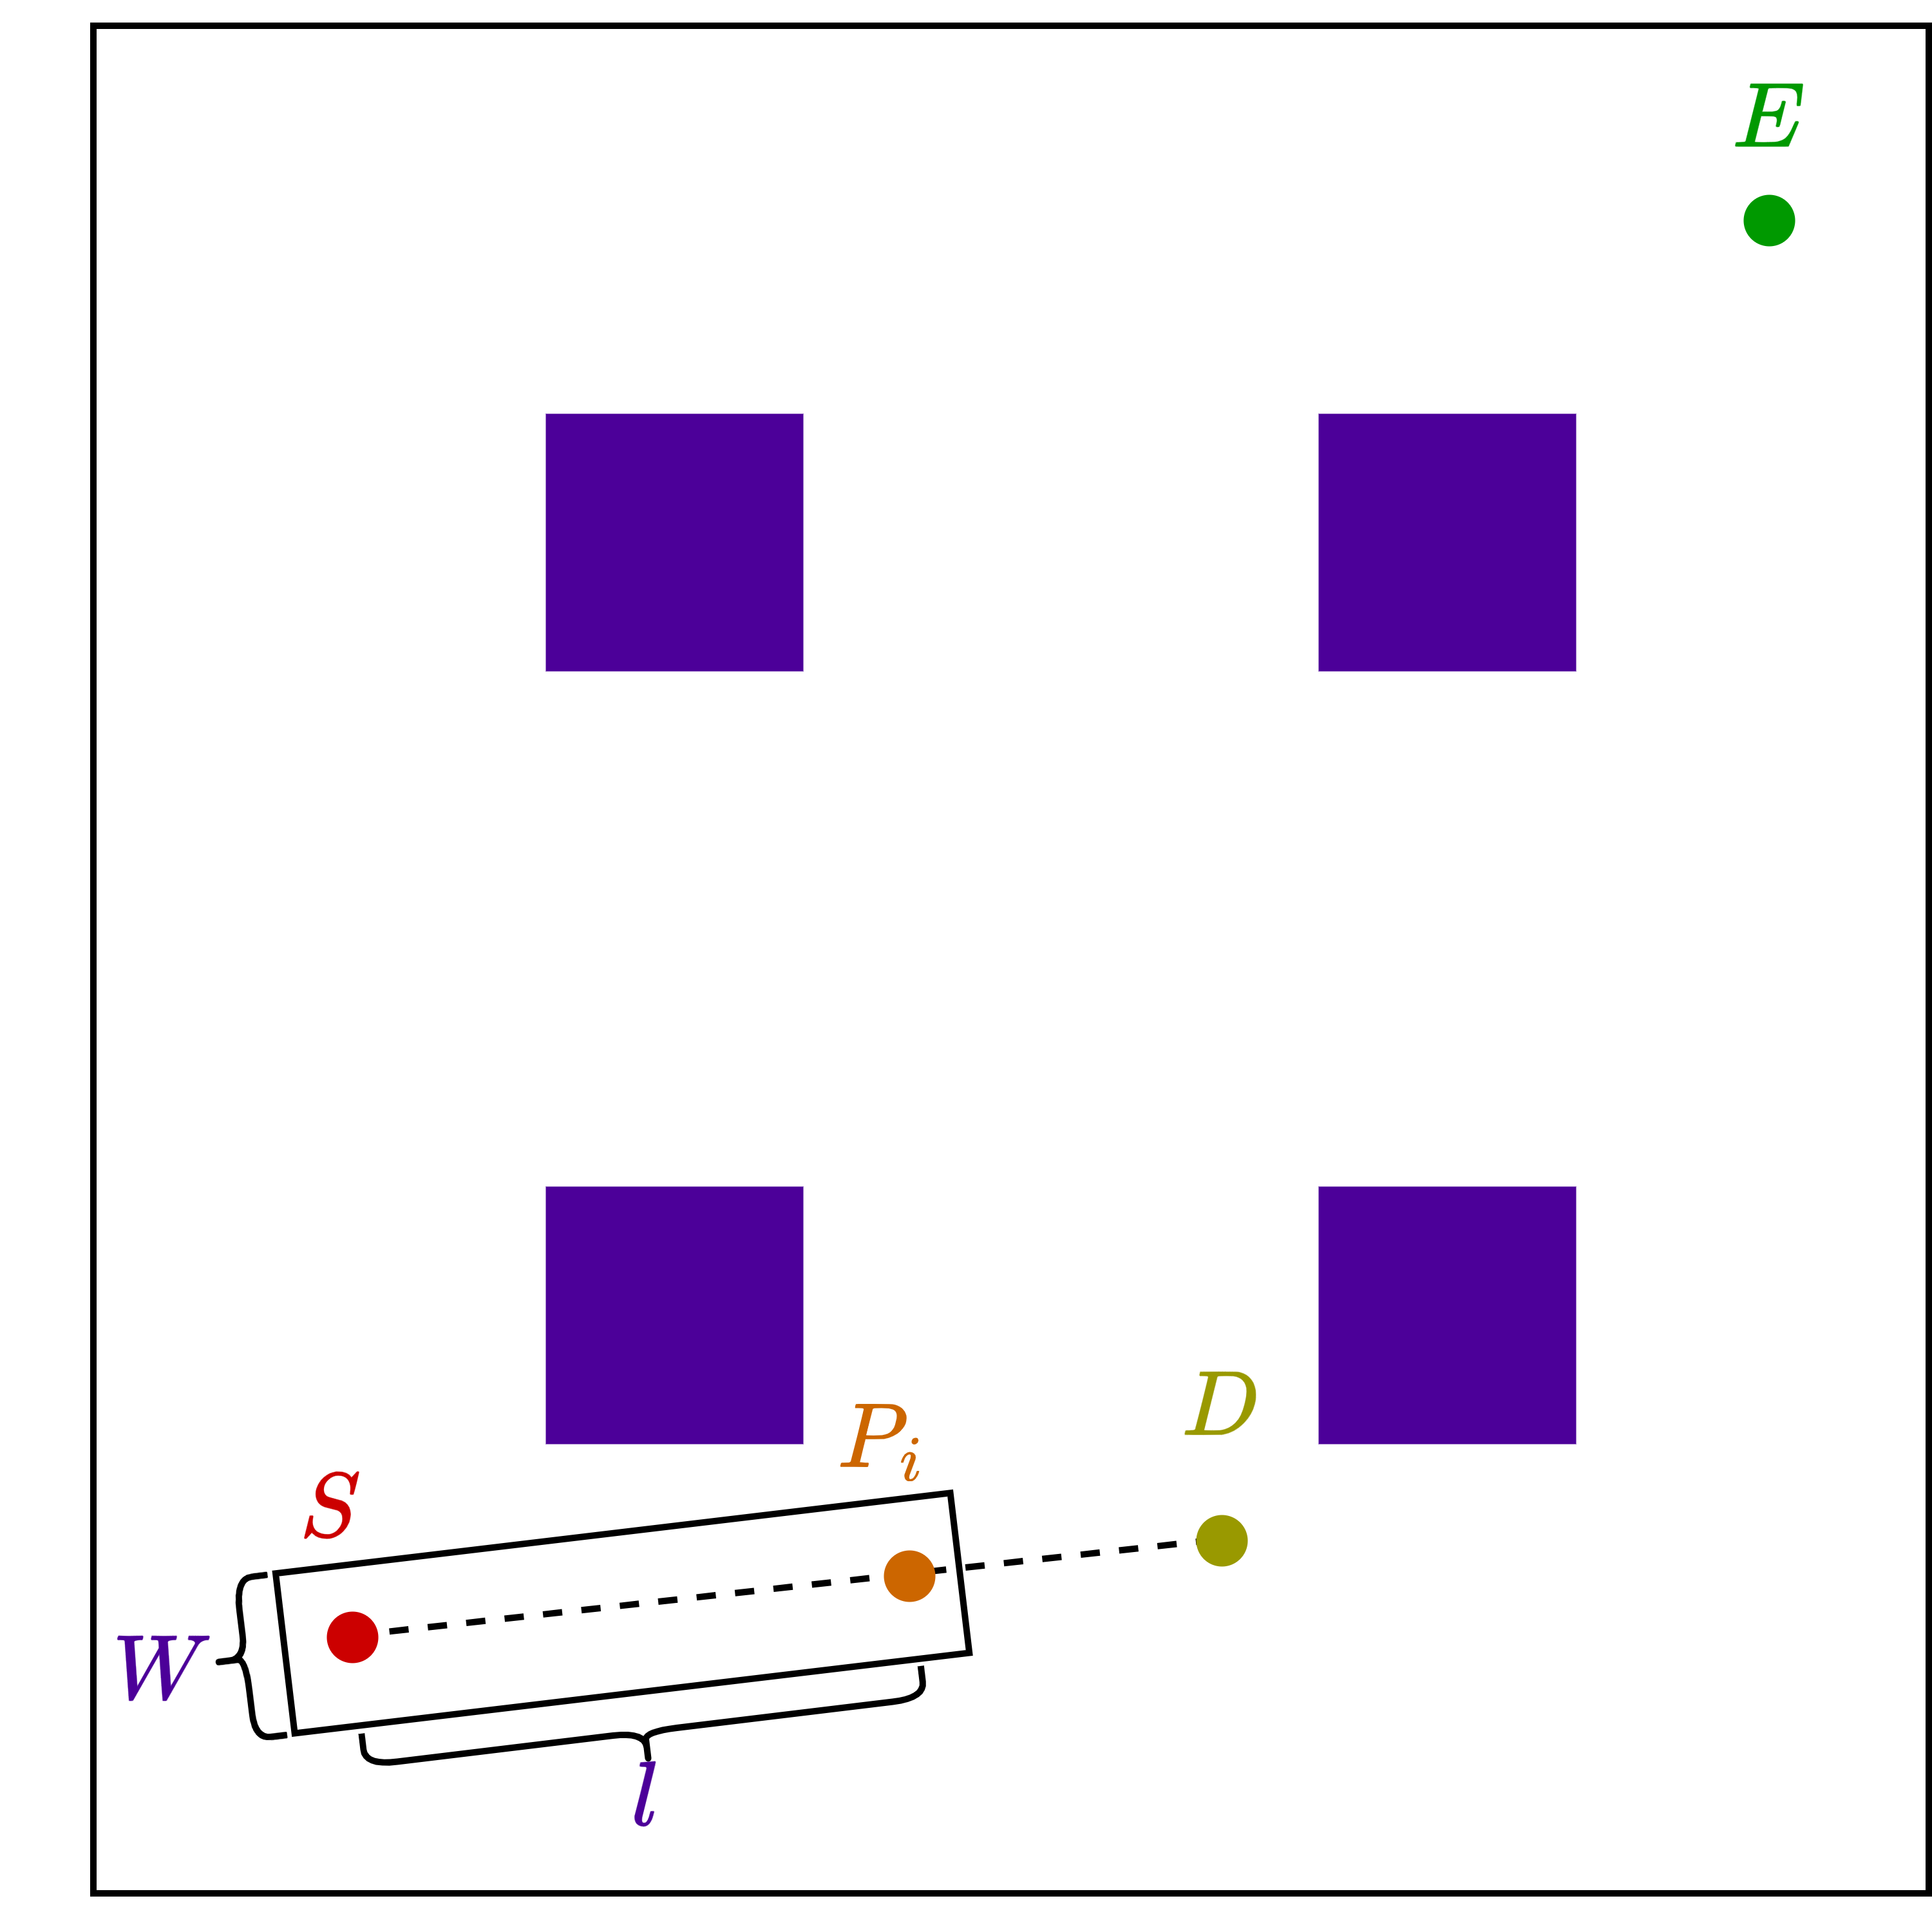
\includegraphics[width=0.95\linewidth]{figs/chap4/RRT_SFC_Geometry.drawio.png}
    \caption{Example of generating first safe flight corridor. Environment is a 2x2 grid of buildings}
    \label{fig:SFC_start}
\end{figure}

\begin{figure}
    \centering
    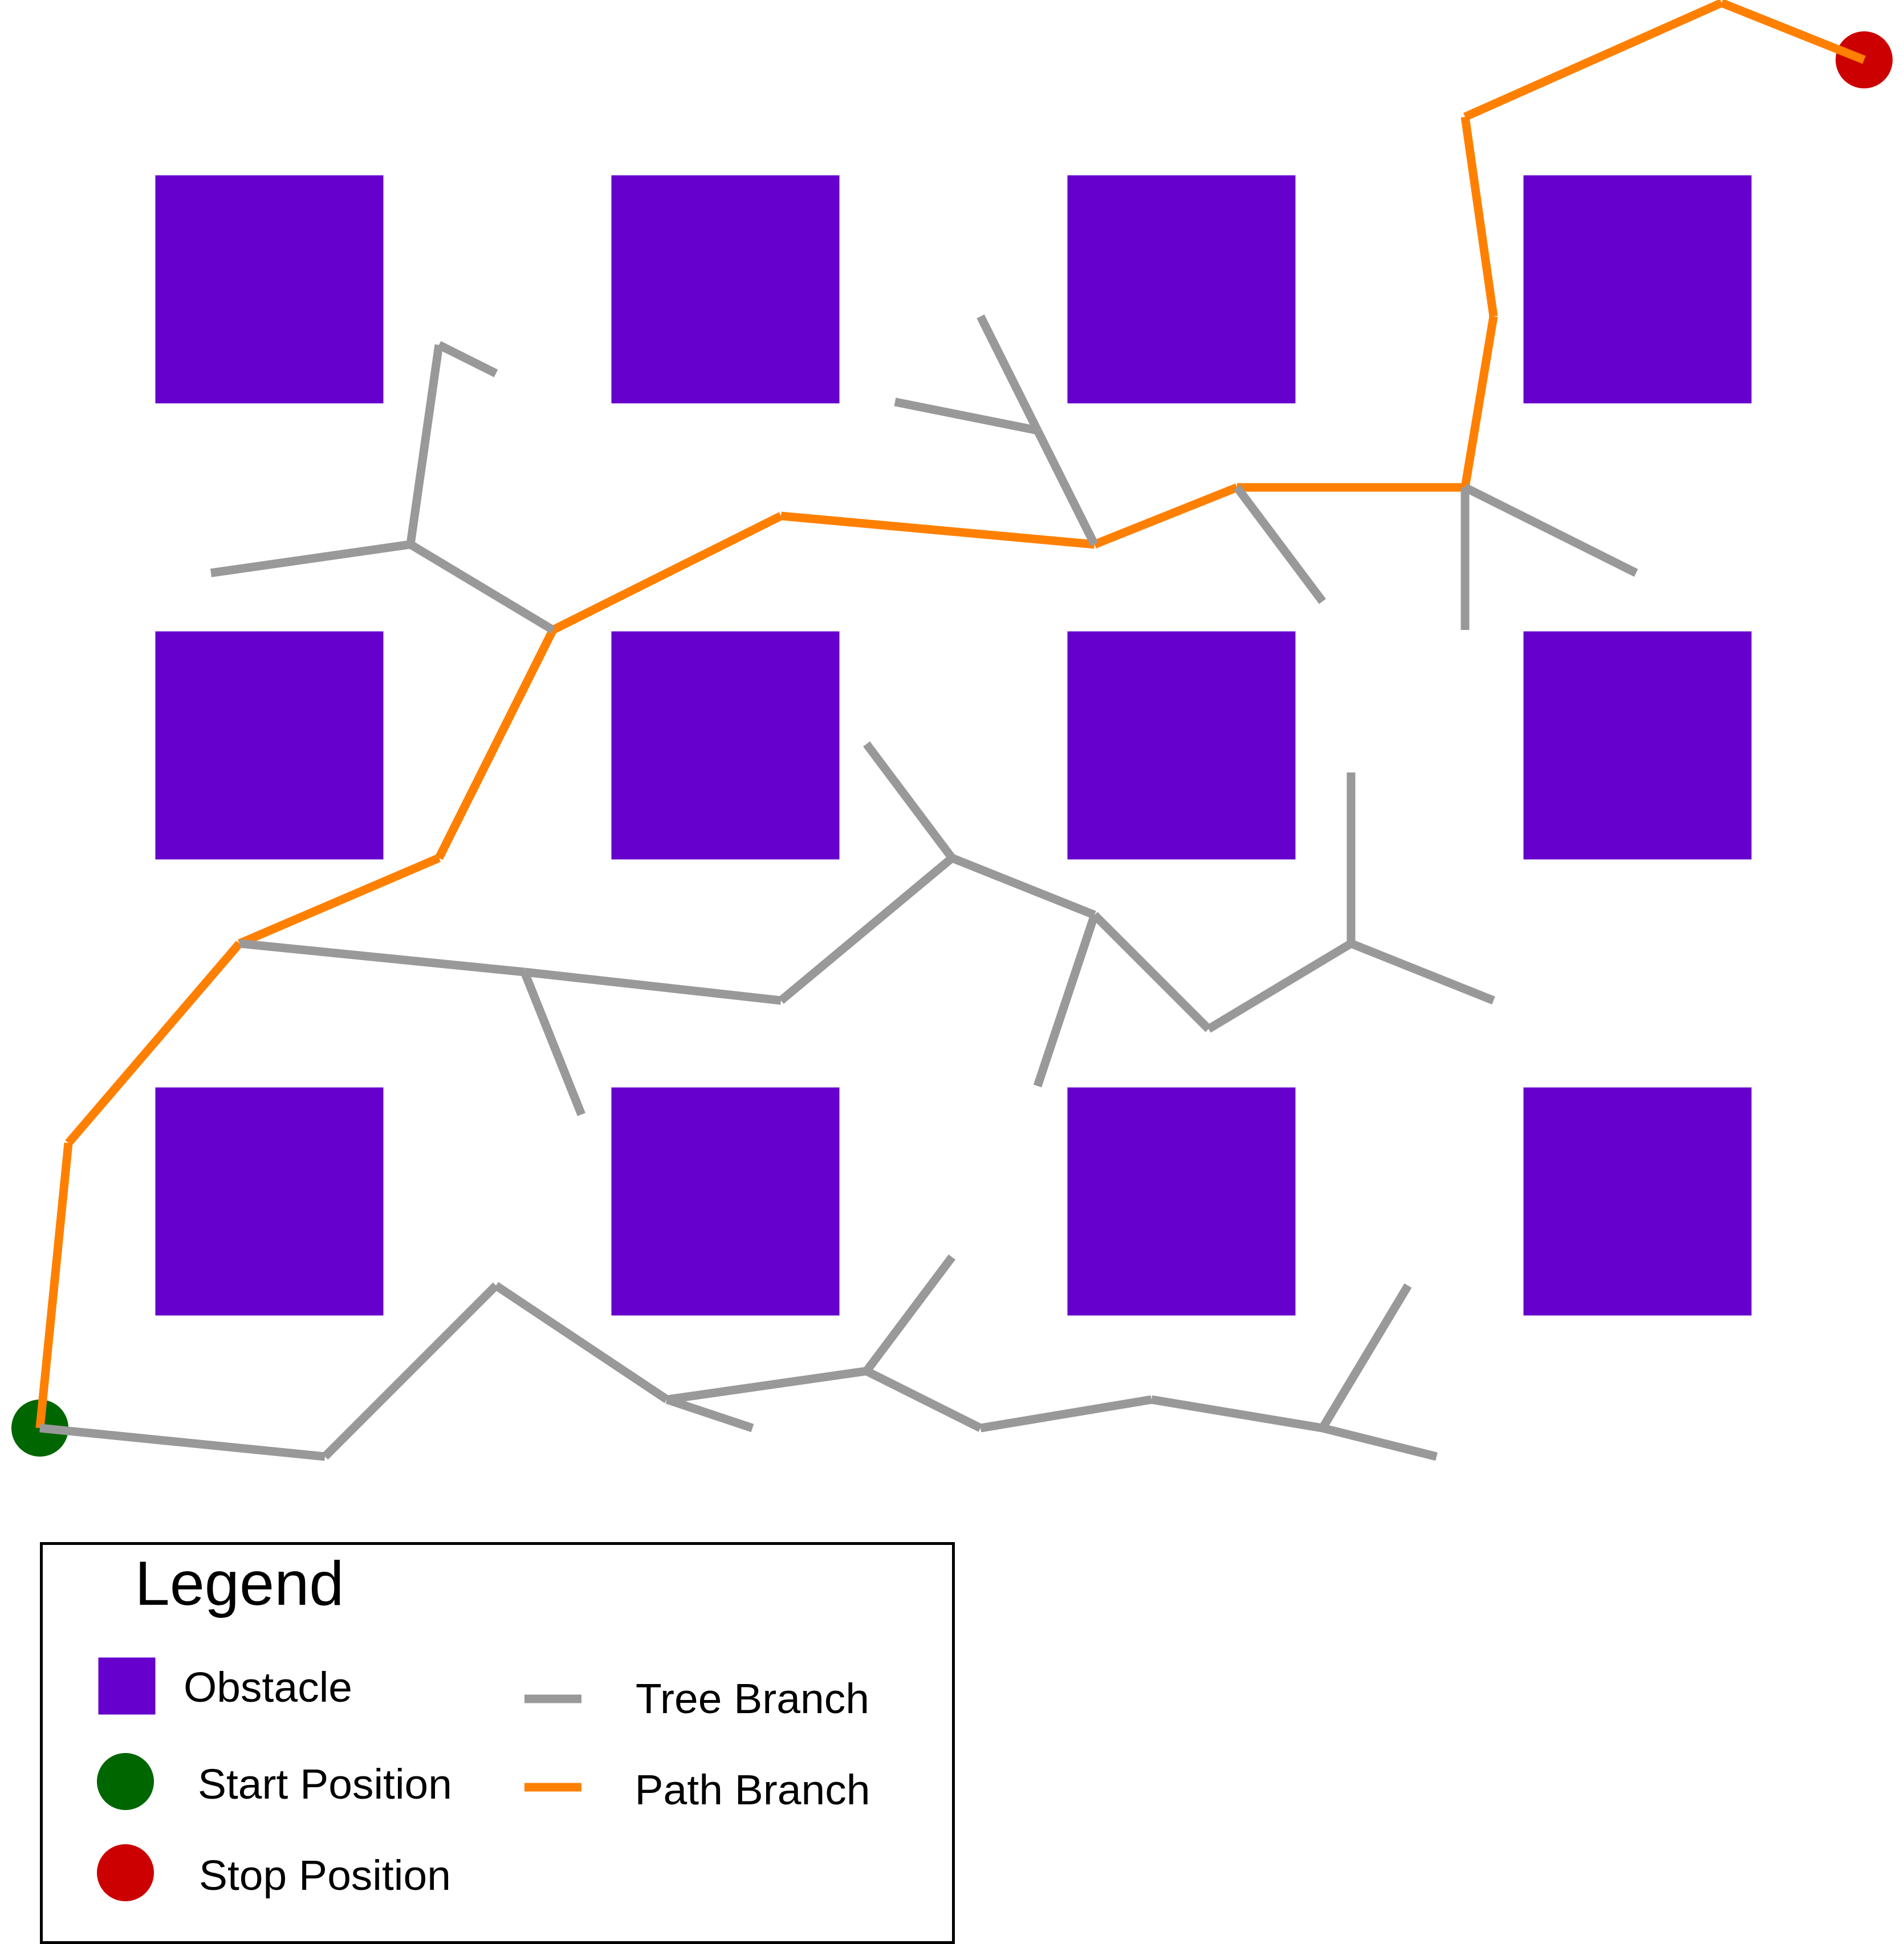
\includegraphics[width=0.75\linewidth]{figs/chap4/RRT Line Example.drawio.png}
    \caption{Straight line RRT example on 4x3 grid of obstacles}
    \label{fig:straight line RRT}
\end{figure}

As shown in Fig. \ref{fig:straight line RRT}, the original algorithm generates a series of connected straight lines, which is the orange path in this figure. 
While this path may be suitable as the actual trajectory for a slow-moving craft like a multi-copter, or a non-holonomic robot, it is not conducive for the trajectory of a fixed-wing aircraft, which has a minimum turning radius and needs to follow a smooth trajectory. 
This straight-line algorithm needs to be modified to a smooth path for any sort of direct trajectory generation. 

RRT* is a common variation of the RRT algorithm which was introduced by \cite{varricchioSamplingbasedAlgorithmsOptimal2014}. 
With traditional RRT, there is no effort to reconnect nodes of the tree to increase efficiency. 
With RRT*, after a new node has been added, it searches among other nodes within a radius for the parent that has the minimum distance. 
With the additional node, the algorithm also searches for other nodes in the region that can have a shorter distance if the new node becomes the parent node. 
While this algorithm eventually converges to an optimal path, it does so under great computational burden due to rewiring after each sample. 

A common variation of RRT is to have it generate Dubins paths instead of straight lines. 
For example, in \cite{yangDubinsPathOrientedRapidly2022} present a method of Dubins path generion using RRT. 
The actual algorithm may be found on page 252 of \cite{uav_book}. 
A trajectory of conglomerated Dubins paths is particularly suited for fixed-wing aircraft to fly. 
An example tree and path are shown in Fig. \ref{fig:dubinsRRT}. 
Unfortunately, no optimization occurs in this algorithm. 
There is also a discontinuity of acceleration at the transition between straight-line and radial flight. 
We desire to create a trajectory using degree 3 B-Splines with optimized distance and continuity of position, velocity, and acceleration.

\begin{figure}
    \centering
    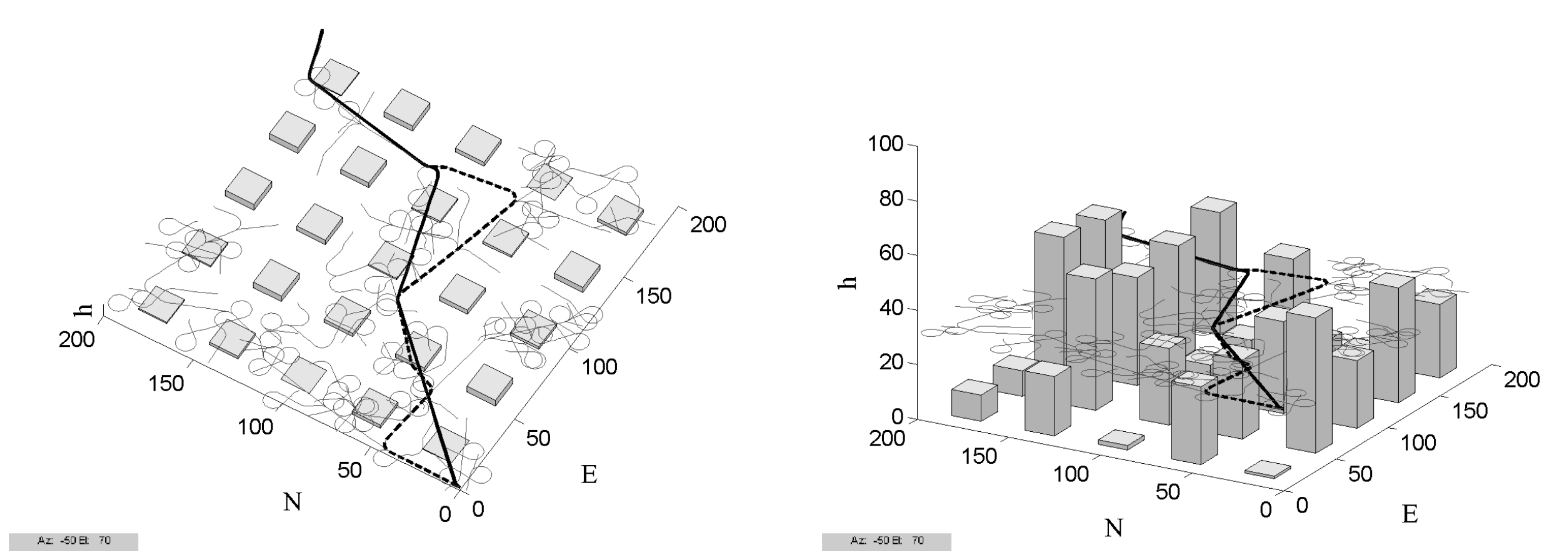
\includegraphics[width=0.95\linewidth]{figs/chap4/dubins rrt.png}
    \caption{RRT algorithm integrating Dubins path into planning. From \cite{uav_book} Fig. 12.12, pg. 255}
    \label{fig:dubinsRRT}
\end{figure}

Many algorithms exist that combine RRT with B-Spline generation. 
For example, \cite{shanDynamicRRTPath2009} presents an RRT algorithm intended for a non holonomic robot. 
The algorithm generates standard straight-line paths and uses points sampled from that path as control points for the final B-Spline path. 
However, this algorithm does not guarantee that the B-Spline does not intersect obstacles in the environment. 
A similar algorithm is presented in \cite{eshtehardianContinuousRRTbasedPath2023} which uses RRT* as the primary search algorithm, and uses the sampled nodes as control points for the B-Spline path. 


\subsection{Safe Flight Corridors}

Safe Flight Corridors are a defined space, which are known to be a safe area for a vehicle to travel inside. 
A corridor is determined to be safe if there is no obstacle or portion of an obstacle within some defined space. 
It is assumed that the obstacles are static; therefore a path remains safe for all time after calculation. 
If a specified corridor or series of corridors remains completely free of obstacles and the aircraft stays within that corridor or series of corridors for its flight period, no collisions will result during that time.


\subsection{Convexity}

Convexity is the property that, for a given function or shape, the line segment between two given points lies above or within that function or shape. 
This is depicted in figure \ref{fig:Convex and Non-Convex Comparison} with two different shapes. 
The left shape contains an internal or reflex angle which precludes the shape from being convex. 

\begin{figure}
    \centering
    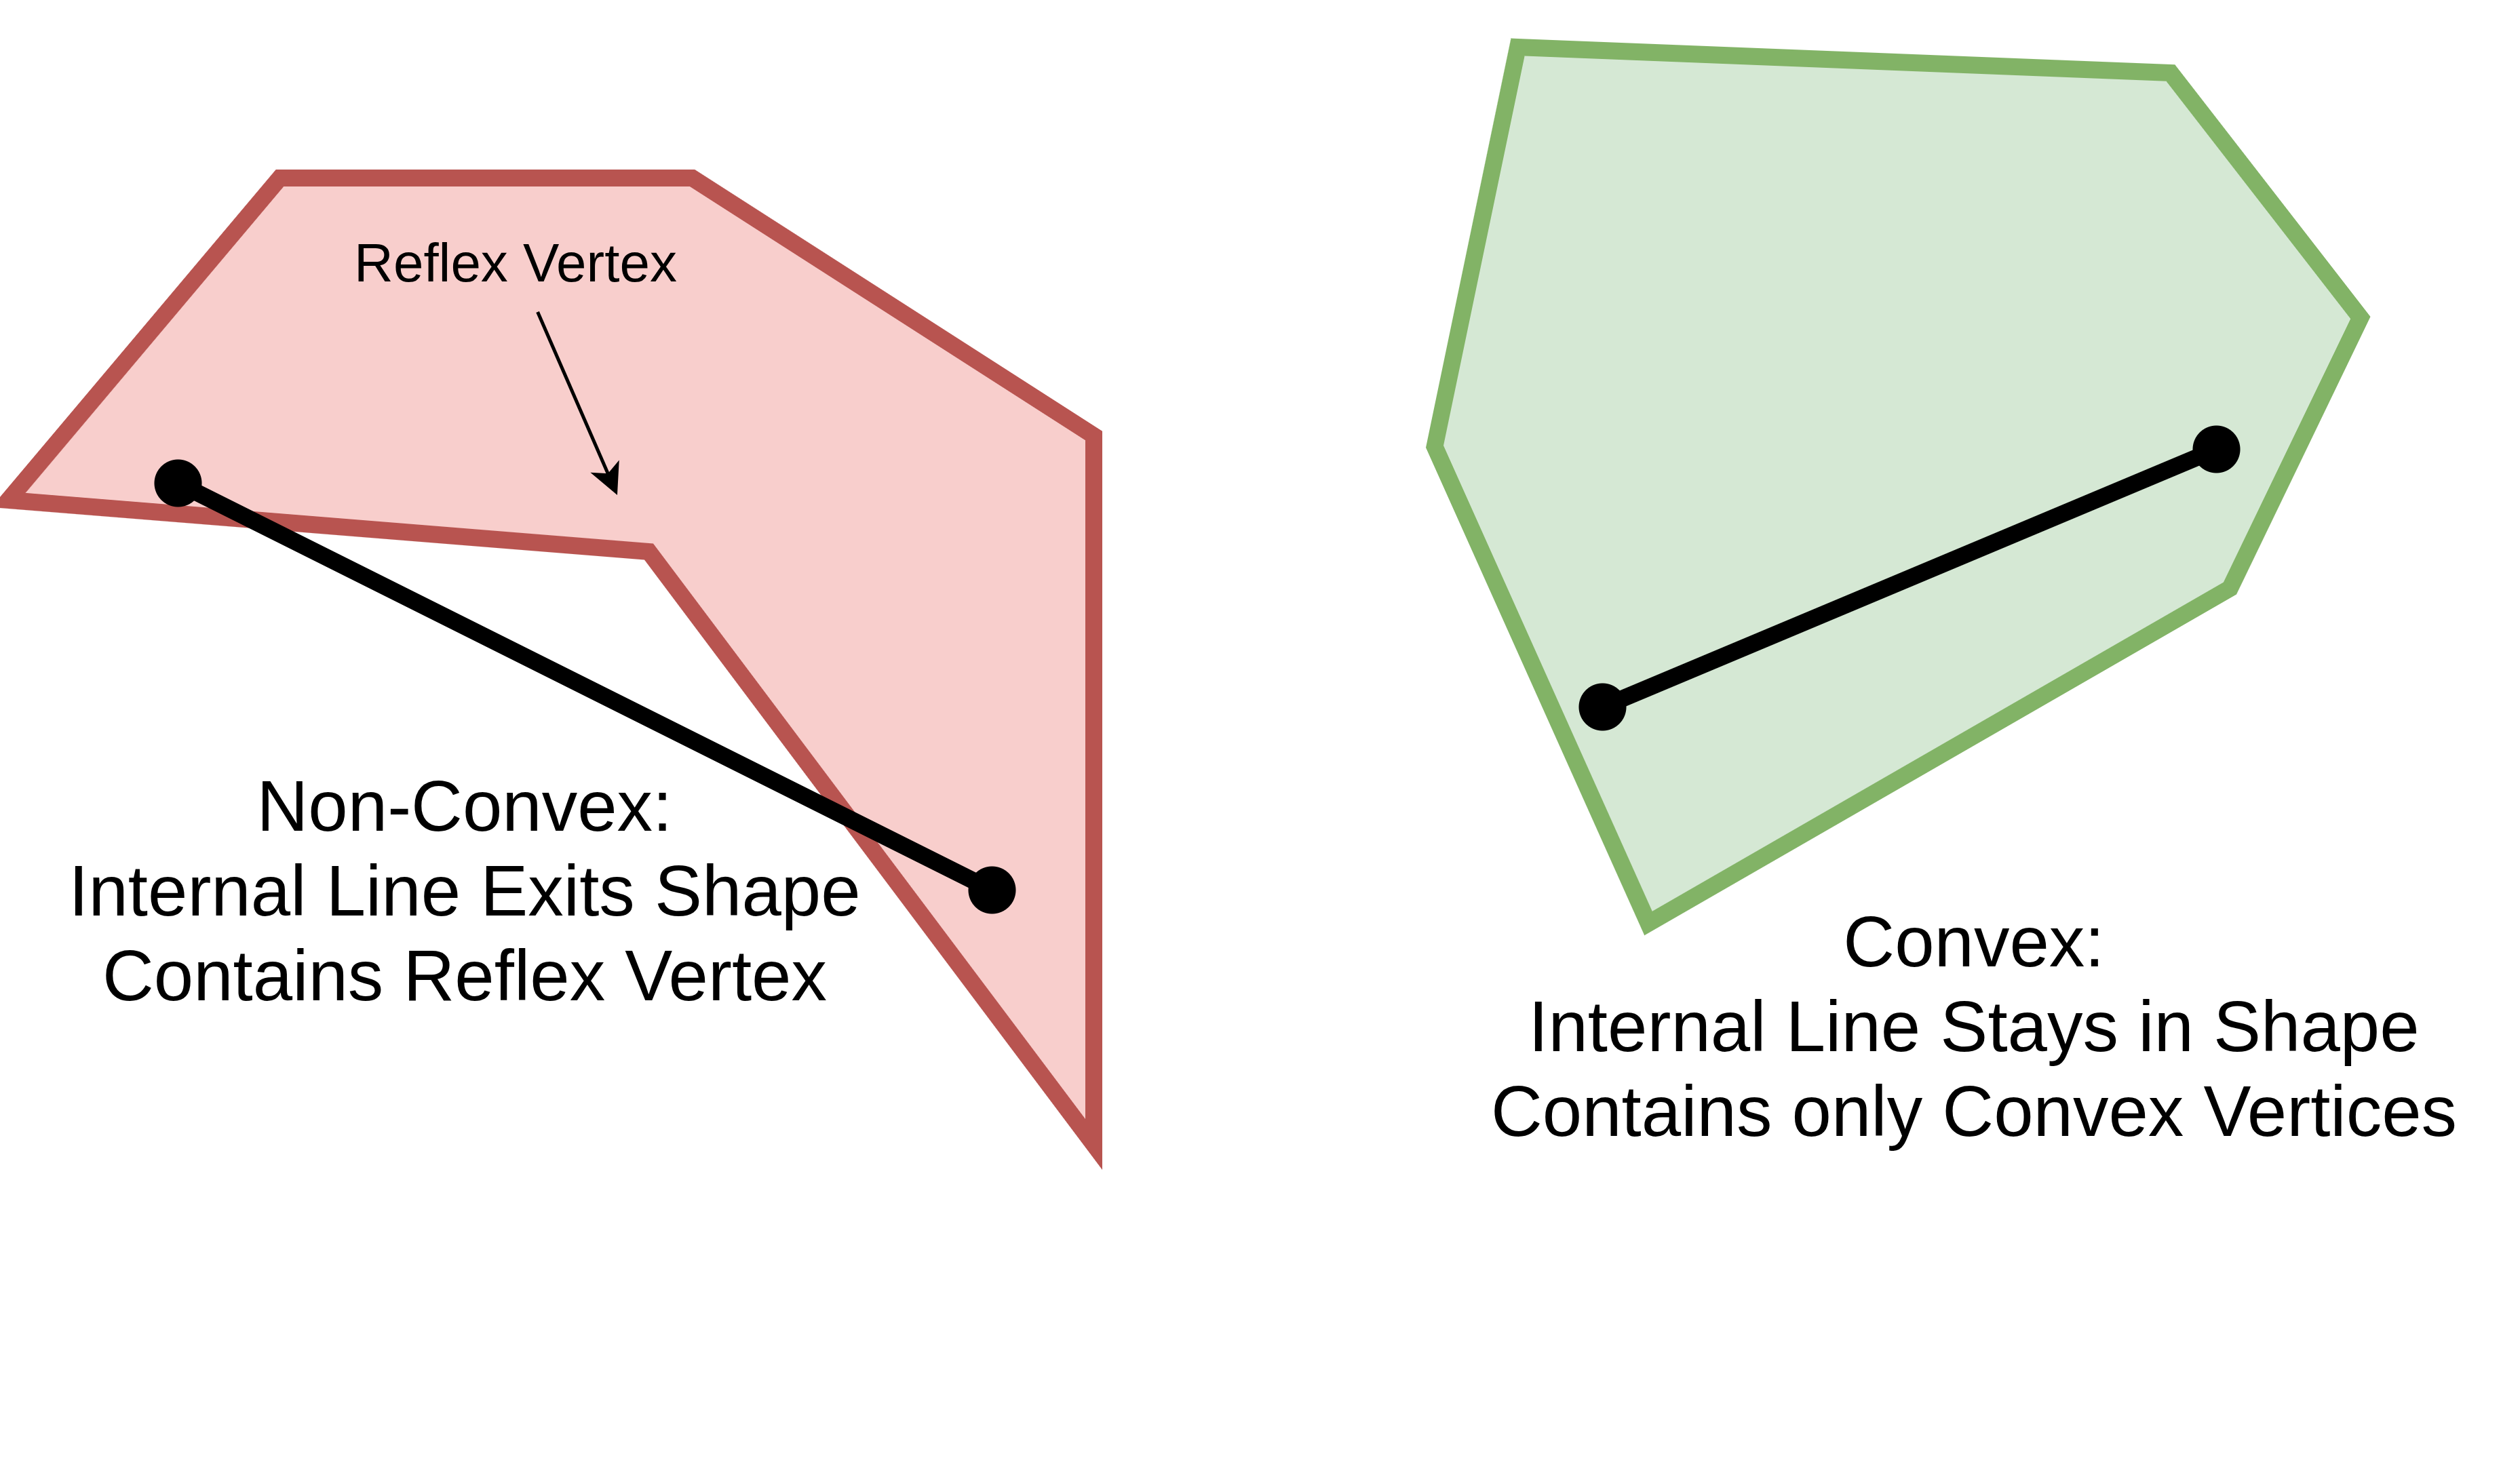
\includegraphics[width=0.75\linewidth]{figs/chap4/Convex and Non-Convex Diagram.drawio.png}
    \caption{An example of a Non-Convex and a Convex shape. A line segment can be drawn between points within the Non-Convex shape and leave the shape temporarily. This is because of the reflex vertex, which has an internal angle greater than $\pi$ radians. Such is not the case with the convex shape, which maintains all internal points.}
    \label{fig:Convex and Non-Convex Comparison}
\end{figure}

Convex polygons are desirable because they can be represented by a linear inequality of the form $Ax \leq b$. 
In other words, a point can be determined to be either inside or outside a polygon using a simple linear inequality. 
The first step to understanding linear inequality constraints comes from half-plane switching criteria, as shown in Fig. \ref{fig:half plane}. 
Given a point $\vec{r}$ on a bisecting line, and a vector normal to that line $\hat{n}$, a point $p$ is on the same half-plane as $\hat{n}$ if $\hat{n}^\top \vec{p} > \hat{n}^\top \vec{r}$.
The point is on the opposite side if the opposite condition is true.

\begin{figure}
    \centering
    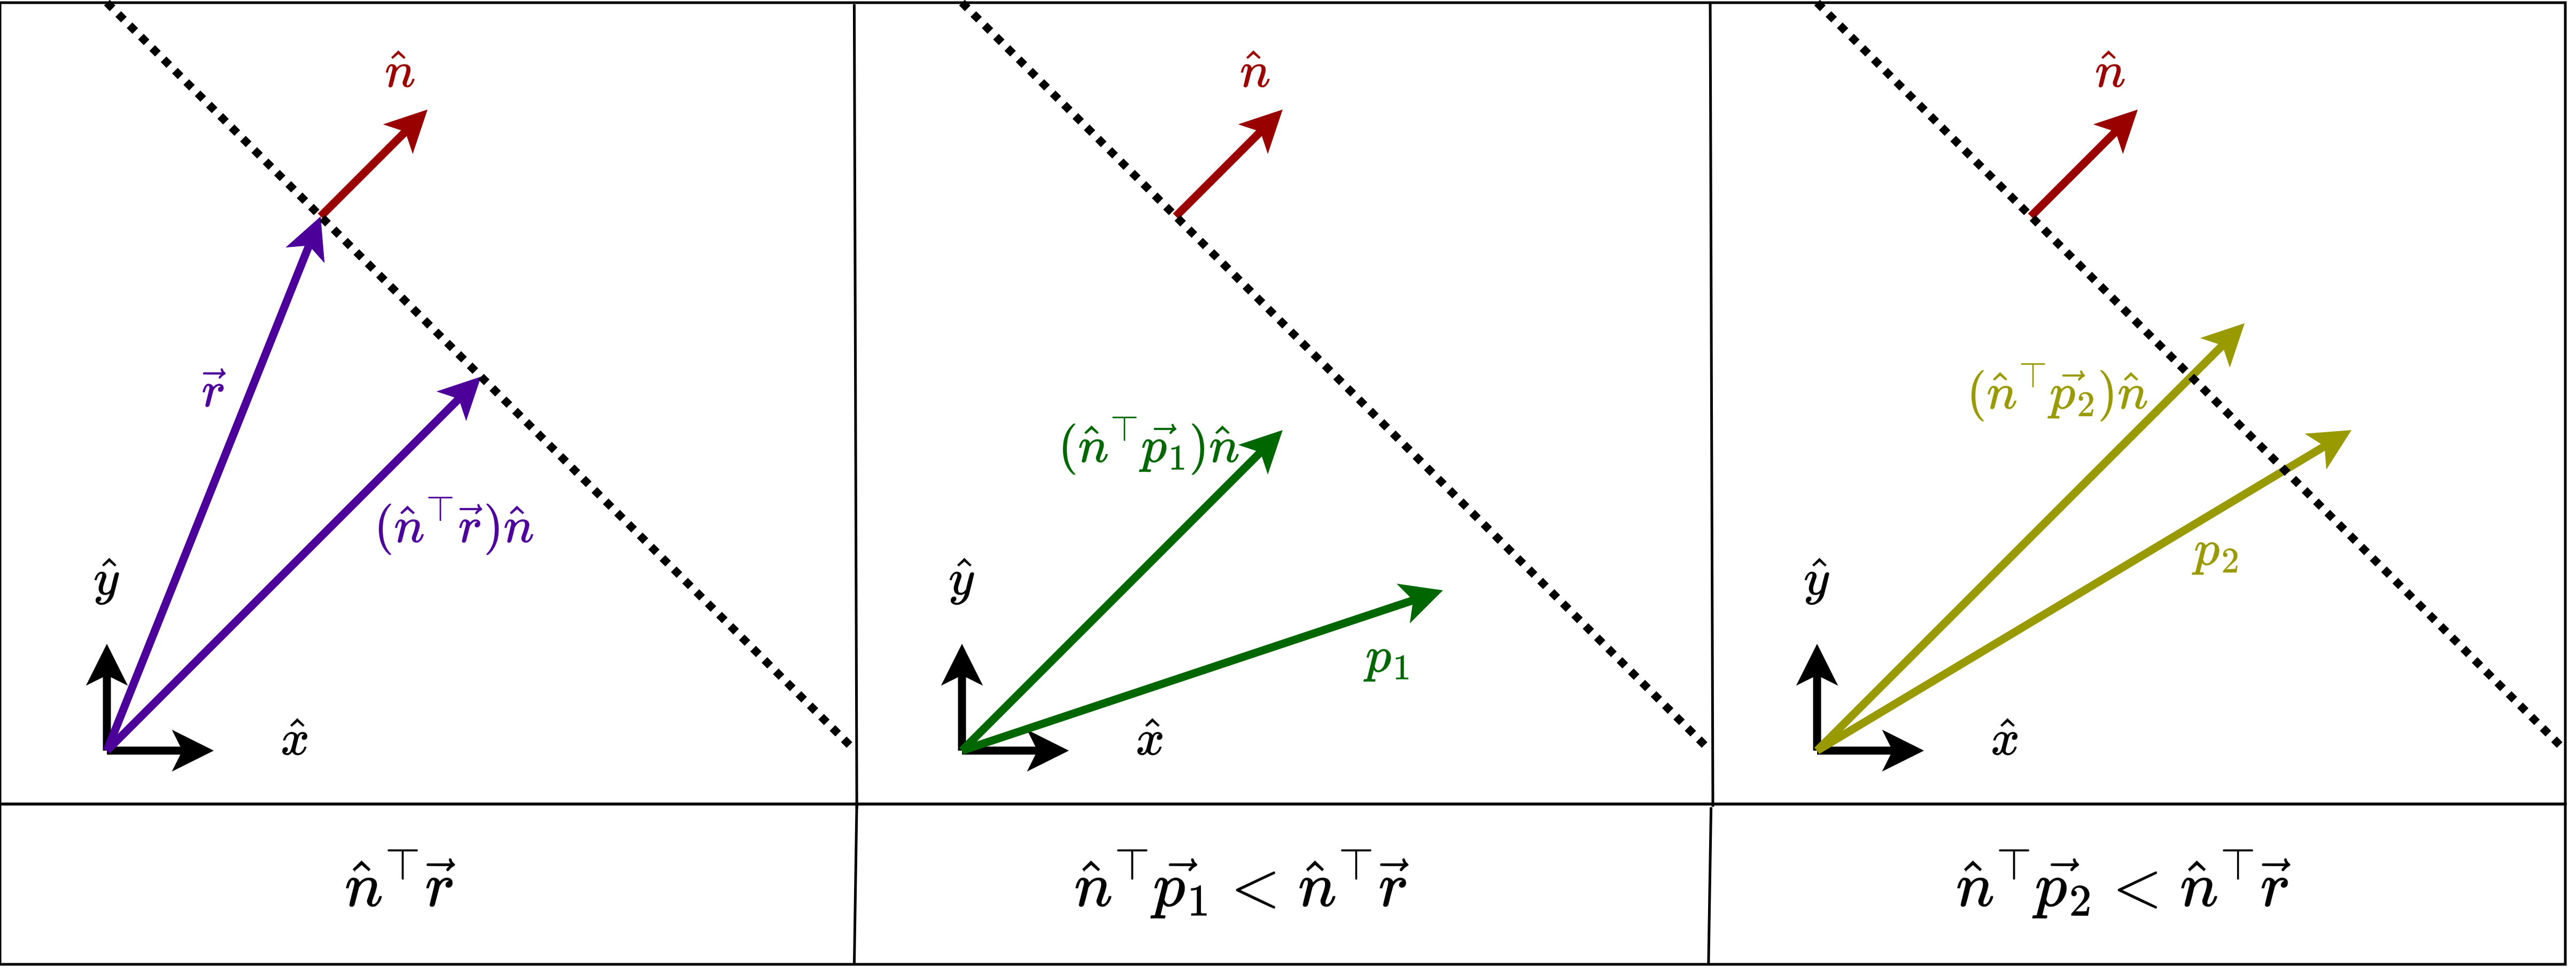
\includegraphics[width=1.0\linewidth]{figs/chap4/Half Plane.drawio.png}
    \caption{Showing geometrical intuition for half-plane switching. $\hat{n}$ represents the vector normal to the half-plane bisecting line, $\vec{r}$ represents an arbitrary point the bisecting line passes through, and $\vec{p_i}$ represents a given point in the plane. This shows three different scenarios: the projections of $\vec{r}$, $\vec{p_1}$, and $\vec{p_2}$ onto $\hat{n}$. $\hat{n}^\top p_1$, is less than $\hat{n}^\top r$ and $(\hat{n}^\top p_1) \hat{n}$ is on the opposite side of the plane as $\hat{n}$, while the opposite is true for $\vec{p_2}$.}
    \label{fig:half plane}
\end{figure}

This equation can be generalized to the form $Ap < b$ where

\begin{align}
    A = 
    \begin{bmatrix}
        \hat{n}^\top\\
    \end{bmatrix}\\
    b = 
    \begin{bmatrix}
        \hat{n}^\top \vec{r}\\
    \end{bmatrix}
\end{align}.

A polygon can be represented as a conglomeration of multiple half-planes, where each edge has its own vectors as $\hat{n}_i$ and $\vec{r}_i$. 
For a convex polygon with $N$ sides, these can be combined into a generalized equation as

\begin{align}
    A =
    \begin{bmatrix}
        \hat{n}_0 & \hat{n}_1 & \hdots & \hat{n}_{N-1}
    \end{bmatrix}^\top\\
    b = 
    \begin{bmatrix}
        \hat{n}_0^\top \vec{r}_0 & 
        \hat{n}_1^\top \vec{r}_1 & 
        \hdots & 
        \hat{n}_{N-1}^\top \vec{r}_{N-1}
    \end{bmatrix}^\top
\end{align}.

An example of a rectangular Safe Flight Corridor is shown in Fig. \ref{fig:single SFC} with normal vectors and a sampled point from each of its four sides. 
For each side $j$ on $SFC_i$ the point $v_{i,j}$ and the normal vector $\hat{n}_{i,j}$ are extracted and input as $\vec{r}_j$ and $\hat{n}_j$ respectively. 

\begin{figure}
    \centering
    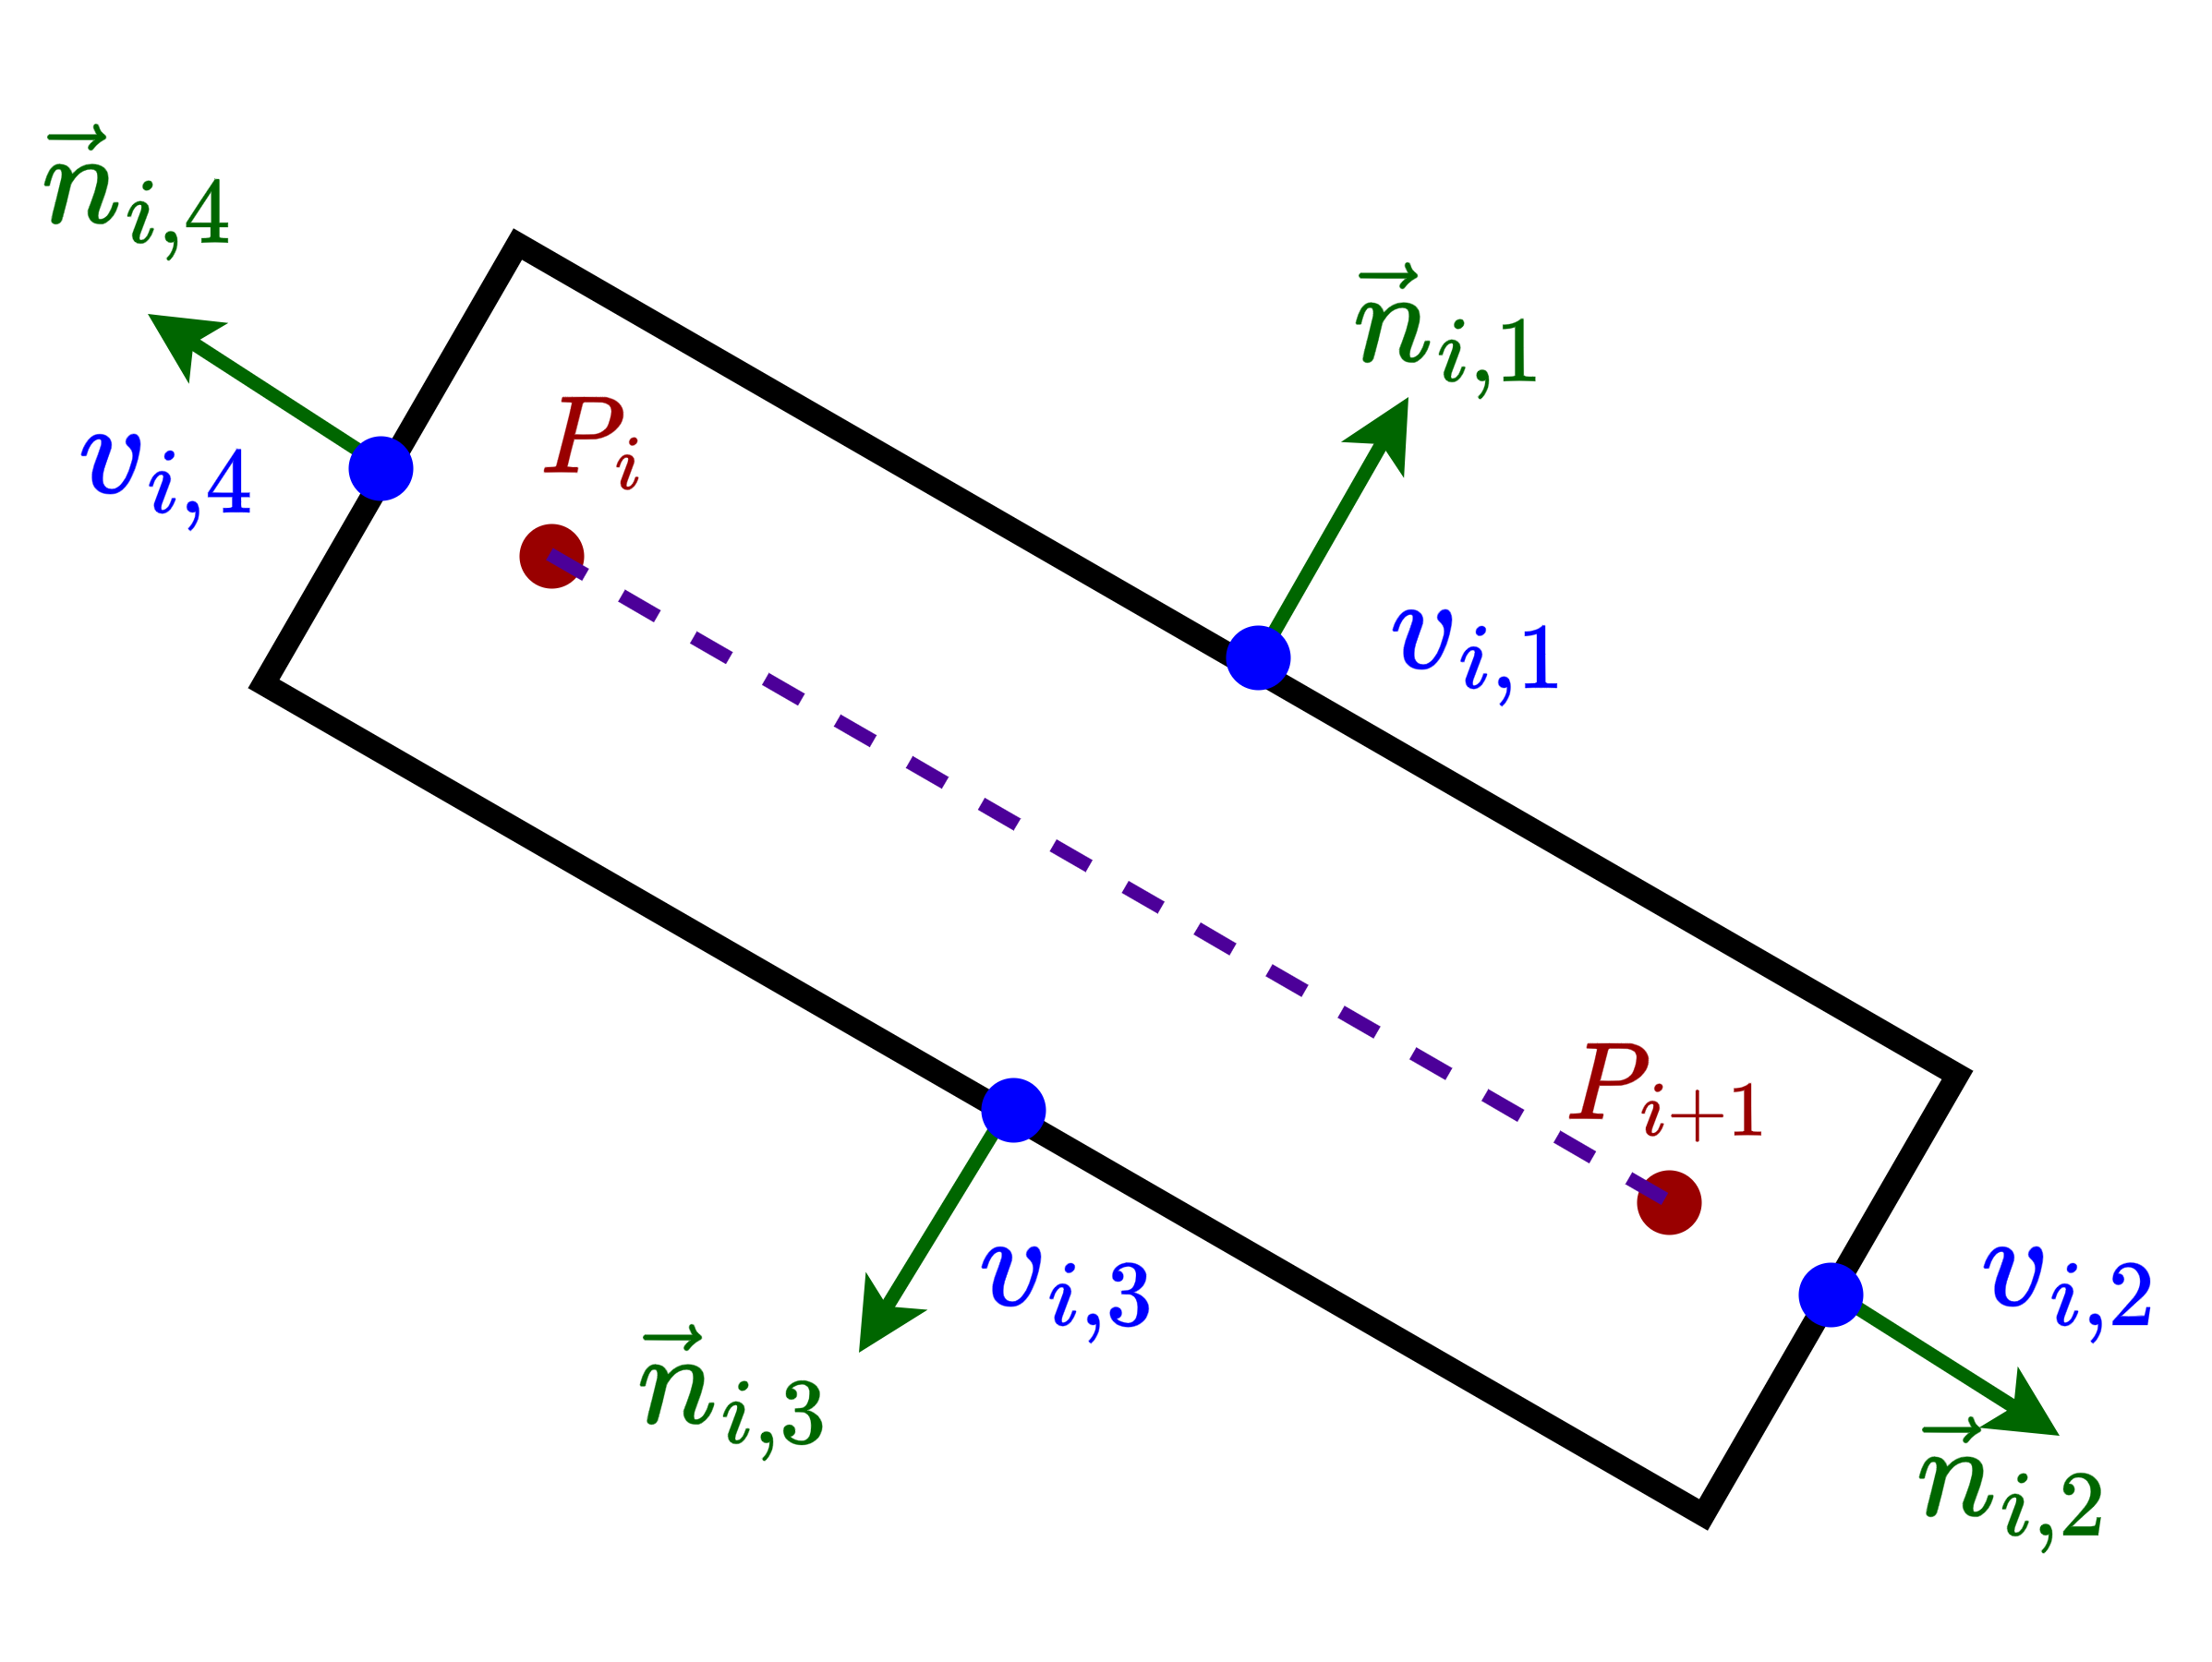
\includegraphics[width=0.5\linewidth]{figs/chap4/SFC Diagram Single.drawio.png}
    \caption{Geometry of rectangular flight corridor, with four normal vectors and vertex points respectively.}
    \label{fig:single SFC}
\end{figure}

\subsection{Enclosure within Safe Flight Corridors}

Although each SFC is a convex set, the union of two or more SFCs is, in general, a non-convex set, as shown in Fig. \ref{fig:non-convex union}. 
The union is a non-convex set, because several sets of points exist for which the joining line exits and re-enters the space. 
For this reason, control points are constrained to either one SFC or the intersection of both SFCs. 

\begin{figure}
    \centering
    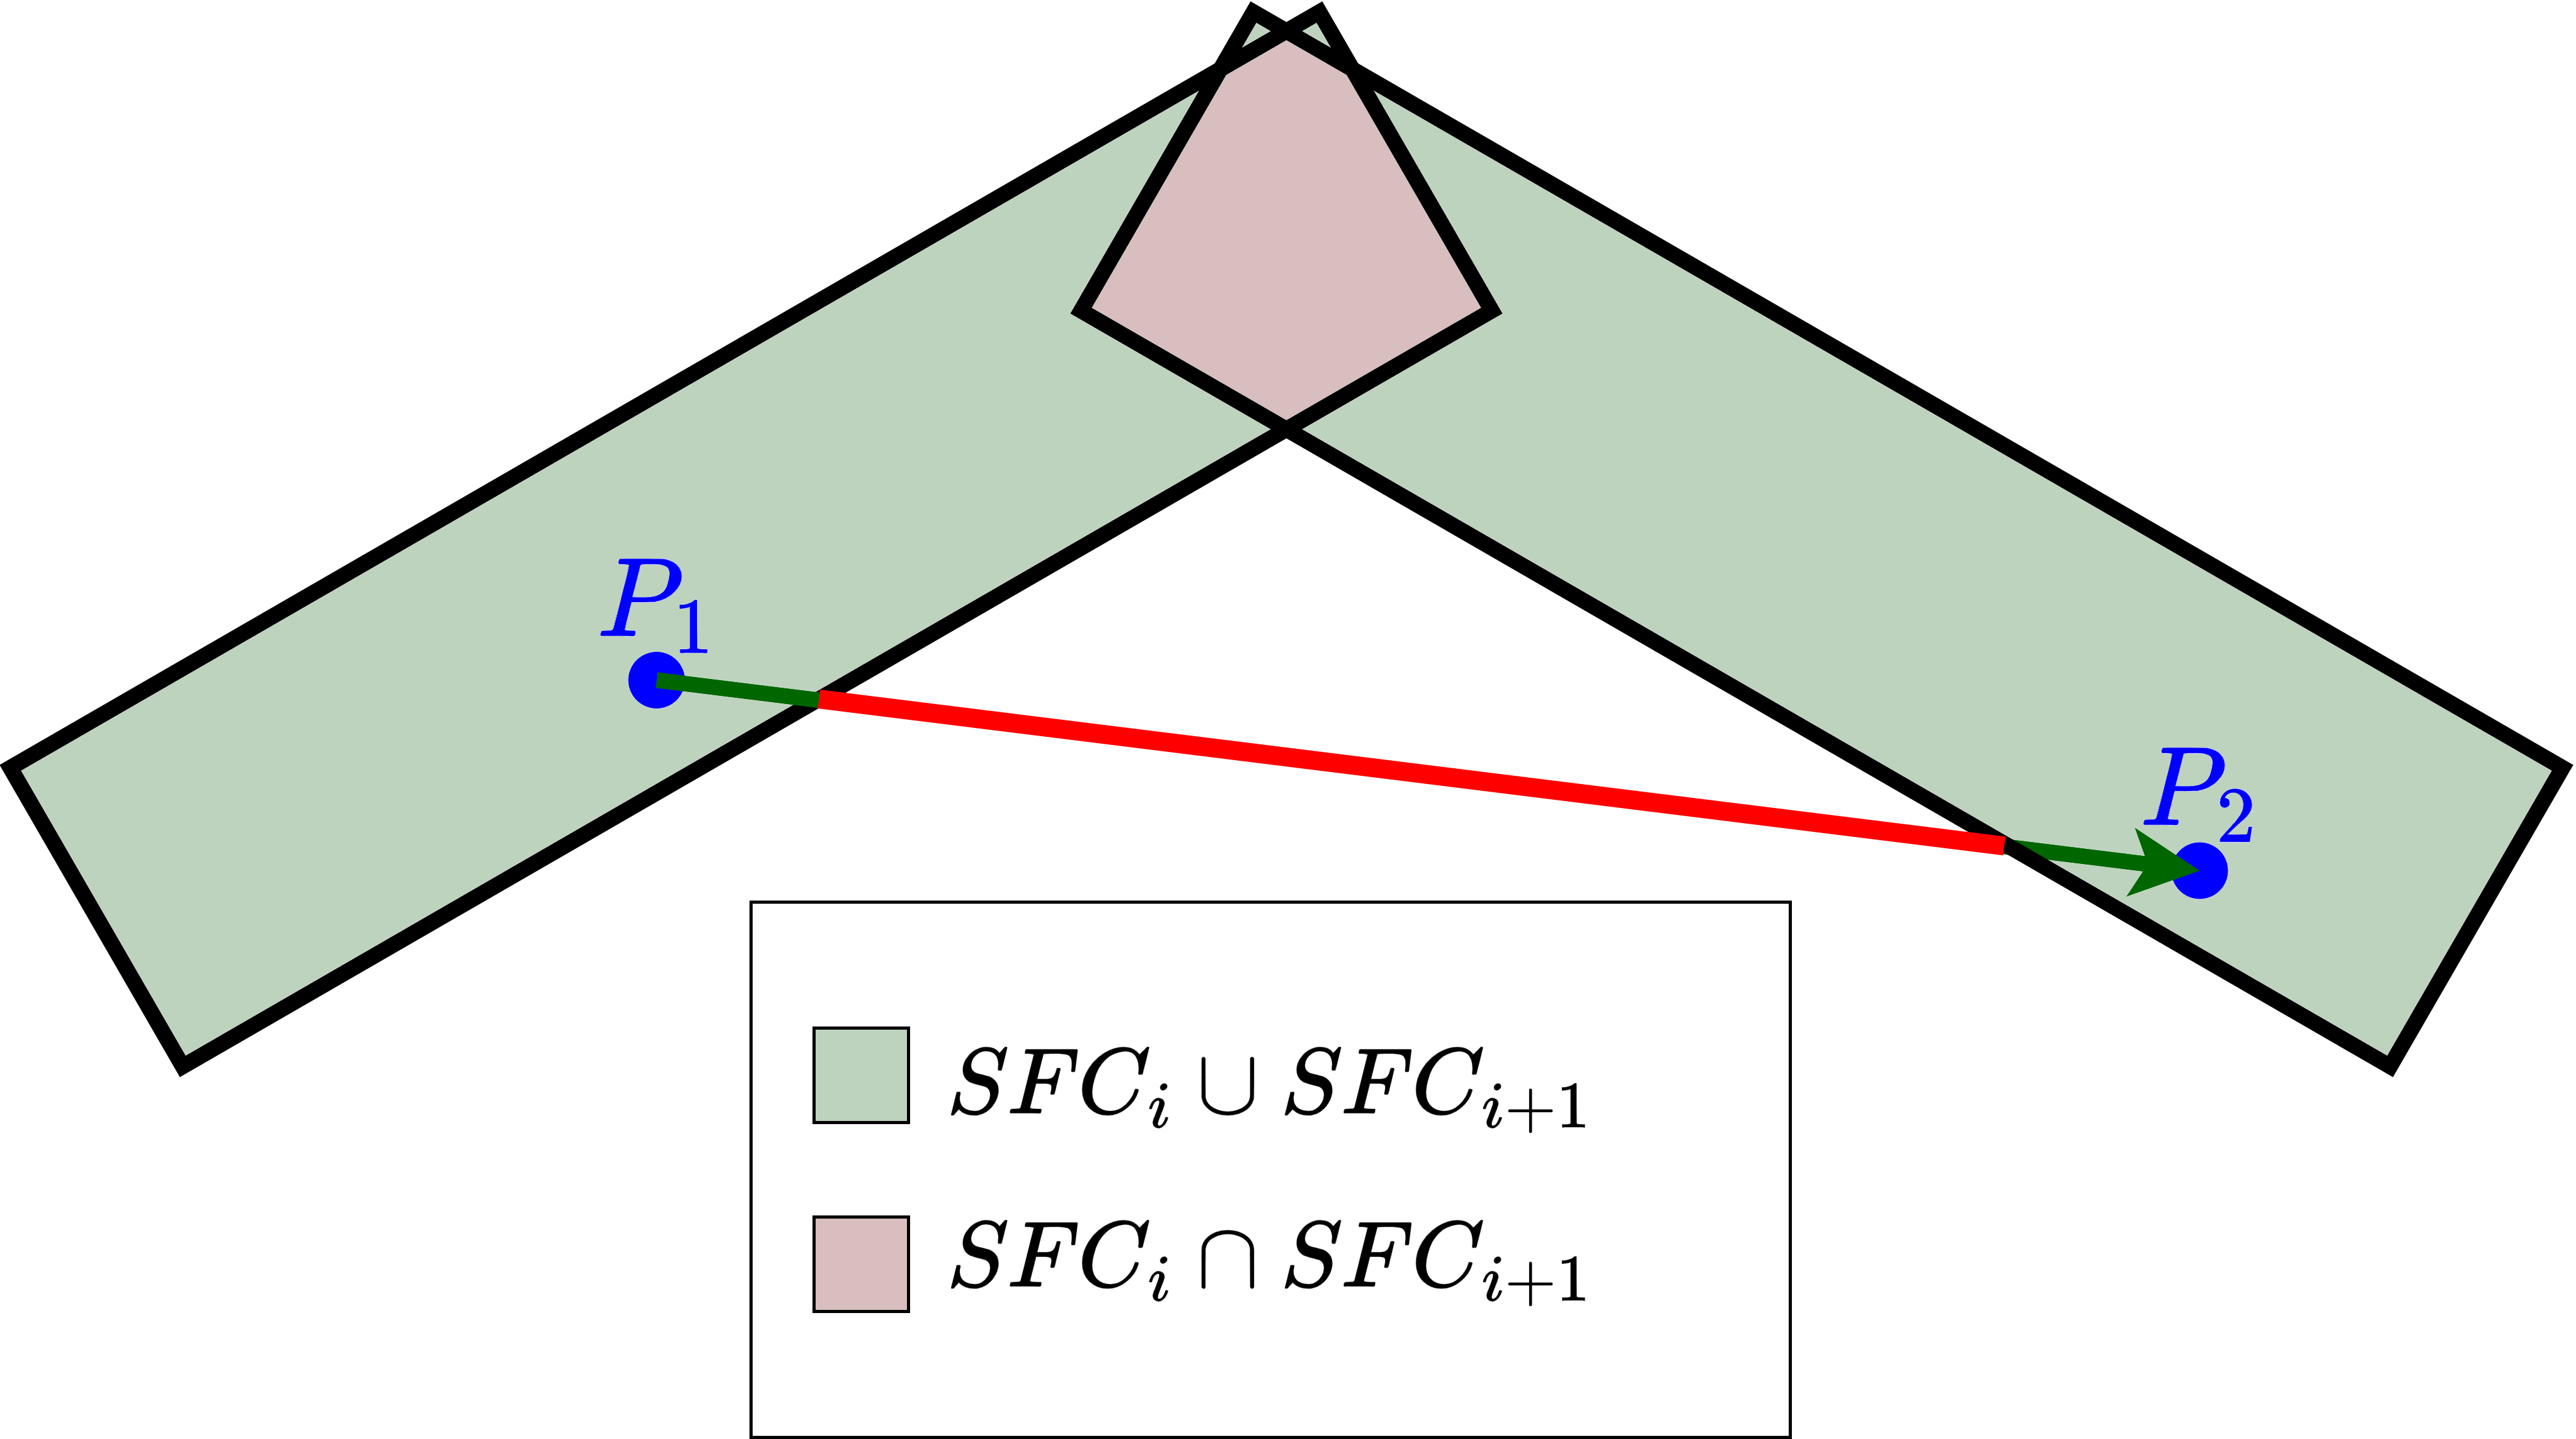
\includegraphics[width=1.0\linewidth]{figs/chap4/SFC Union.drawio (5)_edited.png}
    \caption{Non-convex union of two safe flight corridors}
    \label{fig:non-convex union}
\end{figure}


A major issue with the head-to-tail overlapping method of safe flight corridors is that while each rectangle or rectangular prism is itself a convex hull, and each intersection is also a convex hull, the area or volume of more than one is clearly non-convex in the general case. 
Although each control point may be constrained to an SFC, the convex hull of the control points is not necessarily within an SFC. 
This happens when one or more of a sequential set of $d+1$ control points is not in the same SFC as the others. 
The B-Spline $b(t)$ may cut corners under these conditions.

Fortunately, there is a solution. 
If $d$ control points are constrained to the intersection of $SFC_1$ and $SFC_2$, then each sequential convex hull of control points is within at least one $SFC$. 
For two safe flight corridors with matrices $A_1$ and $A_2$ and vectors $b_1$ and $b_2$, the matrix constraints for the intersection area becomes

\begin{align}
  A_{int} =
    \begin{bmatrix}
      A_1\\
      A_2\\
    \end{bmatrix}\\
  b_{int} =
  \begin{bmatrix}
    b_1\\
    b_2\\
  \end{bmatrix}\\
  A_{int} p < b_{int}
\end{align}.


This is shown in Thm. \ref{thm:overlapping_SFCs}.

\begin{theorem}\label{thm:overlapping_SFCs}
    A set $\mathcal{S}$ is said to be convex iff for every $x_1$ and $x_2$ in $\mathcal{S}$, and every $t \in \left[0,1\right]$, the point $x_3 = tx_1 + (1-t)x_2$ is also in the set $S$. 
    Therefore, the intersection of $\mathcal{S}_1$ and $\mathcal{S}_2$ is also a convex set as: $\mathcal{S}_3 = \mathcal{S}_1 \cap \mathcal{S}_2$.
    
    Given two Safe Flight Corridors $SFC_i$ and $SFC_{i+1}$, existing in dimension $dim$, are defined by the linear inequalities:
    \begin{align}
        SFC_i = \left\{x \in \mathbb{R}^{dim} \space | A_i x \leq b_i\space \right\}\\
        SFC_{i+1} = \left\{x \in \mathbb{R}^{dim} \space | A_{i+1} x \leq b_{i+1}\space \right\}
    \end{align}
    The intersection region of $SFC_i$ and $SFC_{i+1}$ or $\mathcal{P}_i$ is given by:
    \begin{align}
        \mathcal{P}_i = SFC_i \cap SFC_{i+1} = \left\{x \in \mathbb{R}^{dim} \space |
        \begin{bmatrix}
            A_i\\
            A_{i+1}\\
        \end{bmatrix}
        x \leq
        \begin{bmatrix}
            b_i\\
            b_{i+1}\\
        \end{bmatrix}
        \space \right\}
    \end{align}
\end{theorem}

Given these conditions, a B-Spline, $b(t)$ will remain within the set $SFC_i \space \cup \space SFC_{i+1}$ if $d$ sequential control points $\left\{C_j,C_{j+1}, ..., C_{j+d}\right\}$ are constrained to the intersection region $\mathcal{P}_i$ for the transition from $SFC_i$ to $SFC_{i+1}$.

\section{RRT Implementation}

The actual implementation of RRT with safe flight corridors is almost identical to the original straight-line rrt implementation.
This algorithm is given as

\begin{algorithm}
    \caption{SFC RRT}
    \begin{algorithmic}[1]
    \While{Path not found}
        \State Random sample within space
        \State Find nearest existing end node
        \State Draw line between sample and nearest node

        \If{length $> \ell$}
            \State Candidate node $\ell$ away on line
        \Else
            \State Candidate node at new node
        \EndIf

        \State Create candidate SFC with nearest node and candidate node

        \If{Candidate node intersects any obstacle}
            \State Return and start over
        \Else
            \State Add candidate node to tree

            \If{Candidate node close to end}
                \State Create SFC with candidate node and end point

                \If{End candidate intersects}
                    \State Break
                \Else
                    \State Return path found
                \EndIf
            \EndIf
        \EndIf
    \EndWhile
    \end{algorithmic}
\end{algorithm}.


An example of a resultant tree is shown in Fig. \ref{fig:rrt tree example}.

\begin{figure}
    \centering
    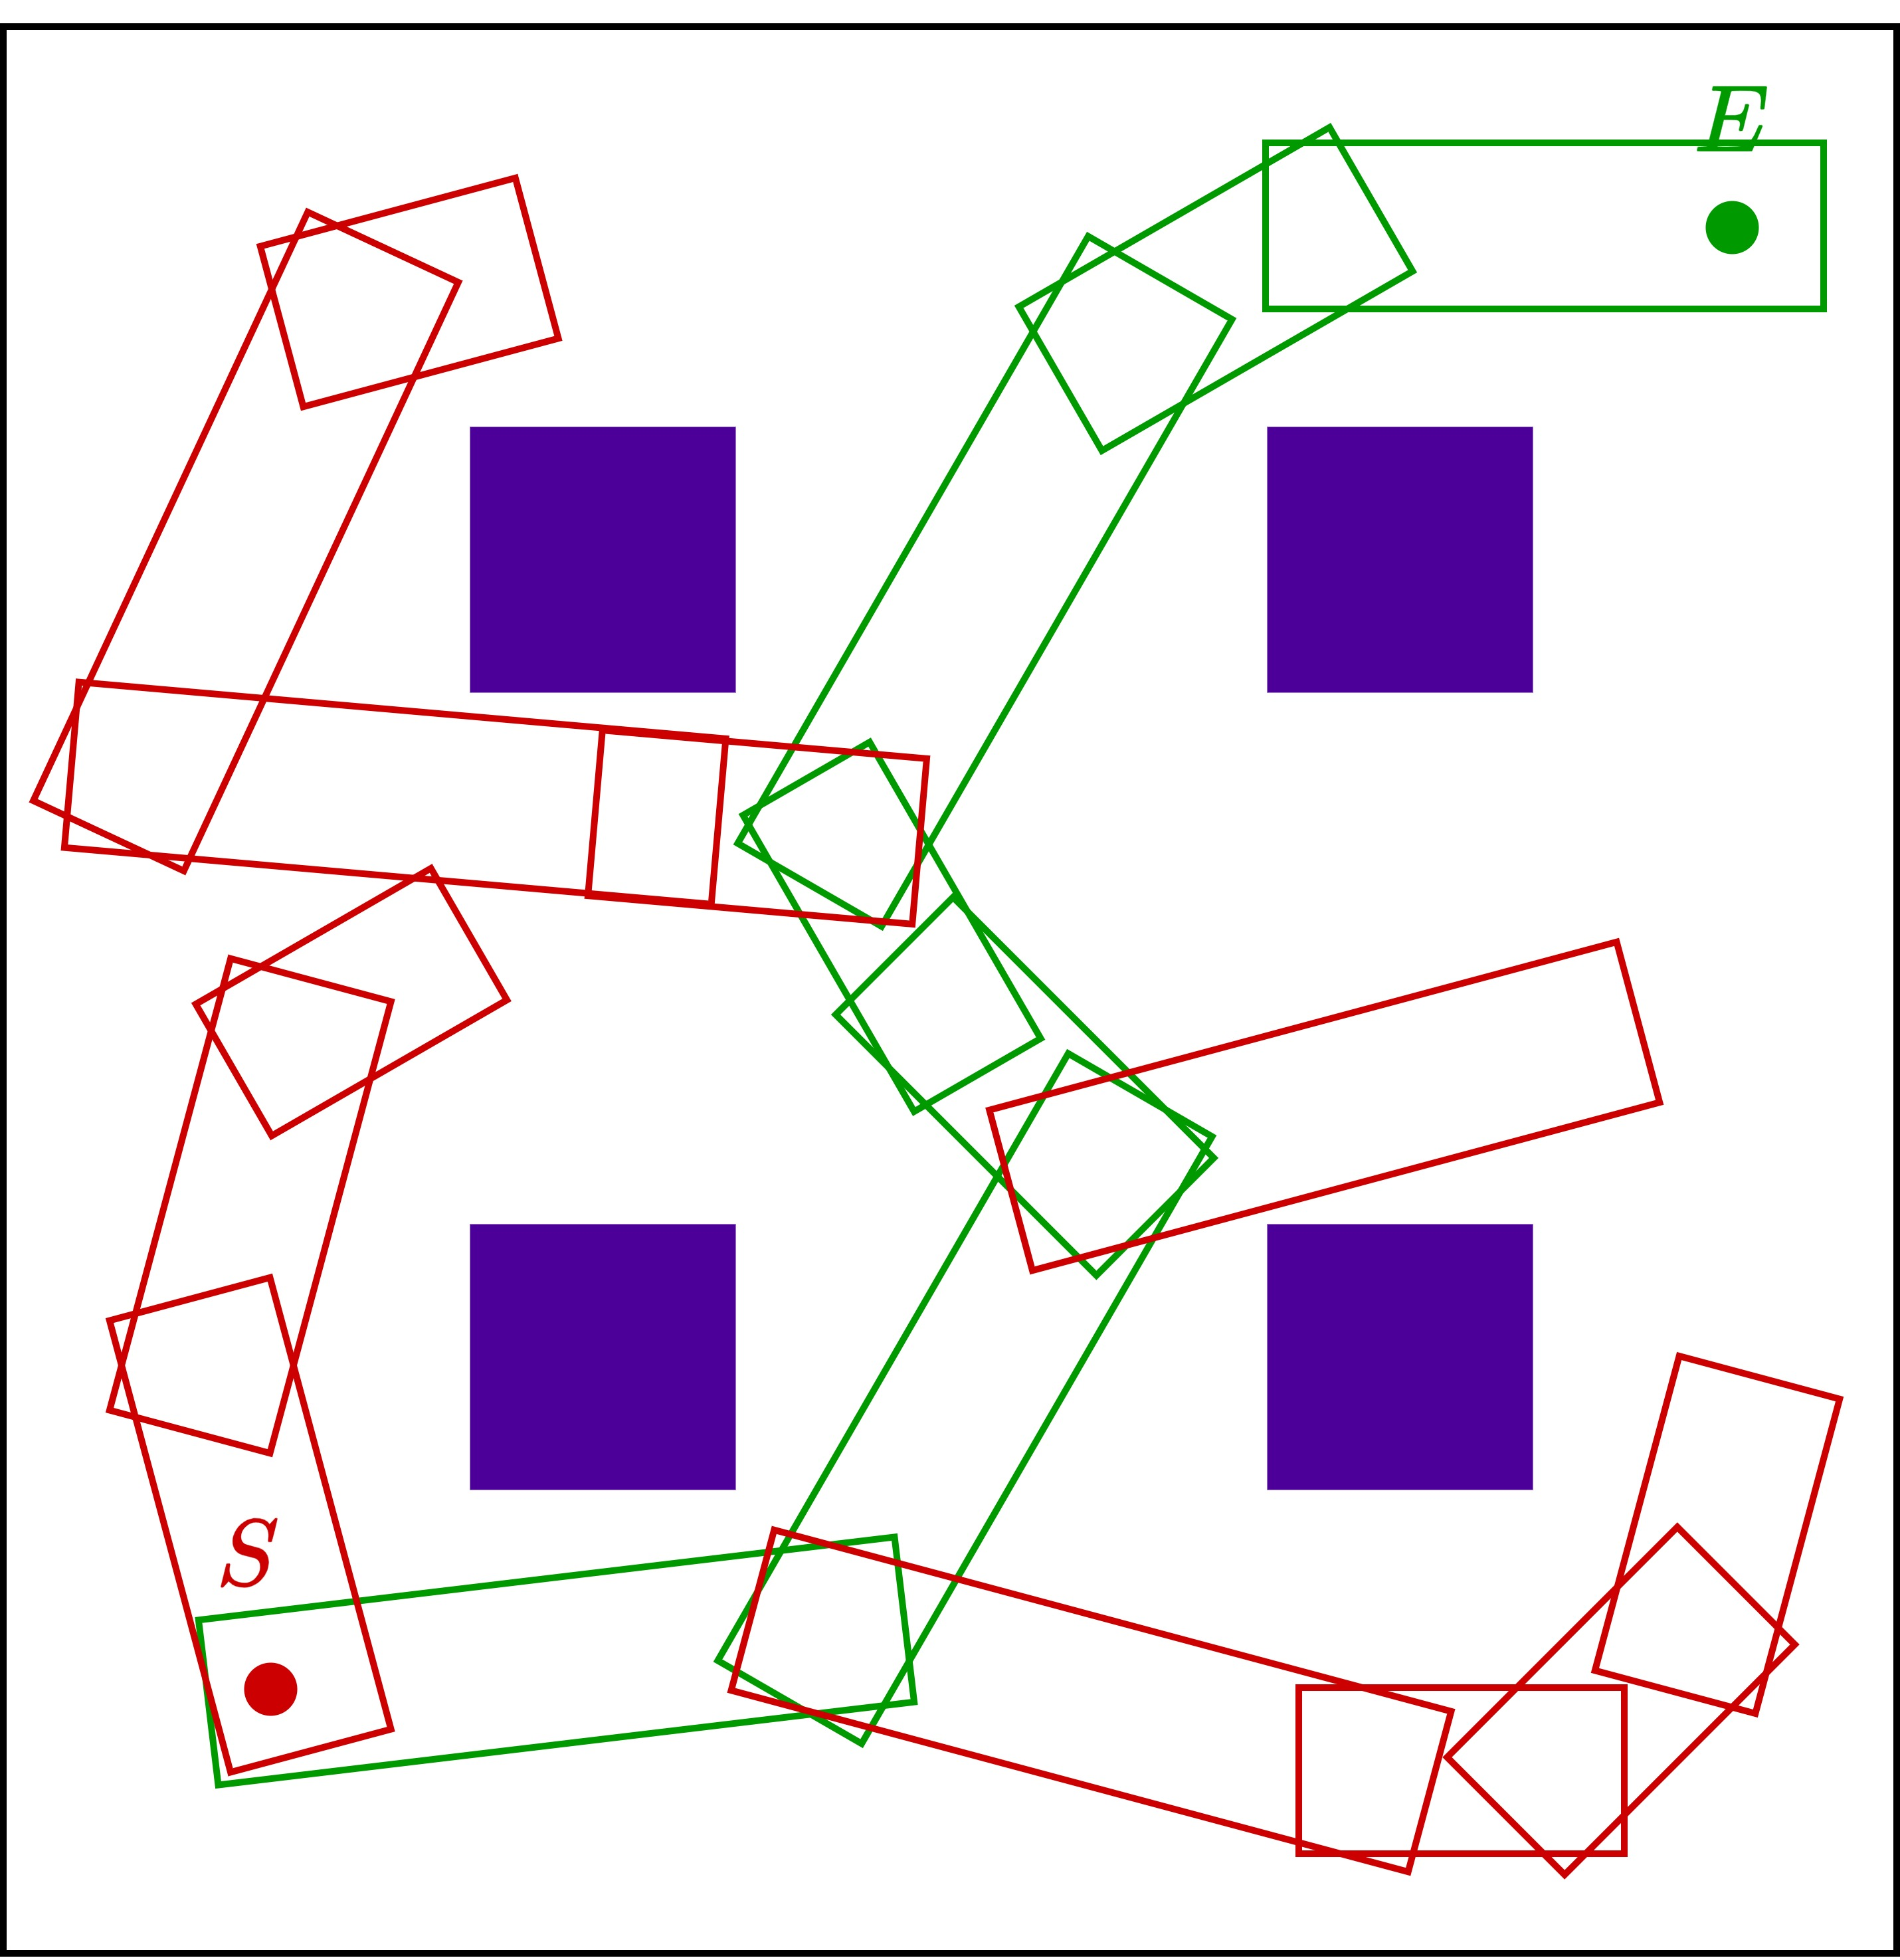
\includegraphics[width=0.9\linewidth]{figs/chap4/RRT Example Tree.jpg}
    \caption{Example of RRT tree.}
    \label{fig:rrt tree example}
\end{figure}


\subsection{Obstacle Intersection}

During the RRT algorithm, it is necessary to determine whether a candidate Safe Flight Corridor intersects an obstacle.
There must be a method to determine if any part of an SFC overlaps with any part of an obstacle.
This is accomplished using linear constraints, as depicted in Fig. \ref{fig:obstacleIntersection}.

\begin{figure}
    \centering
    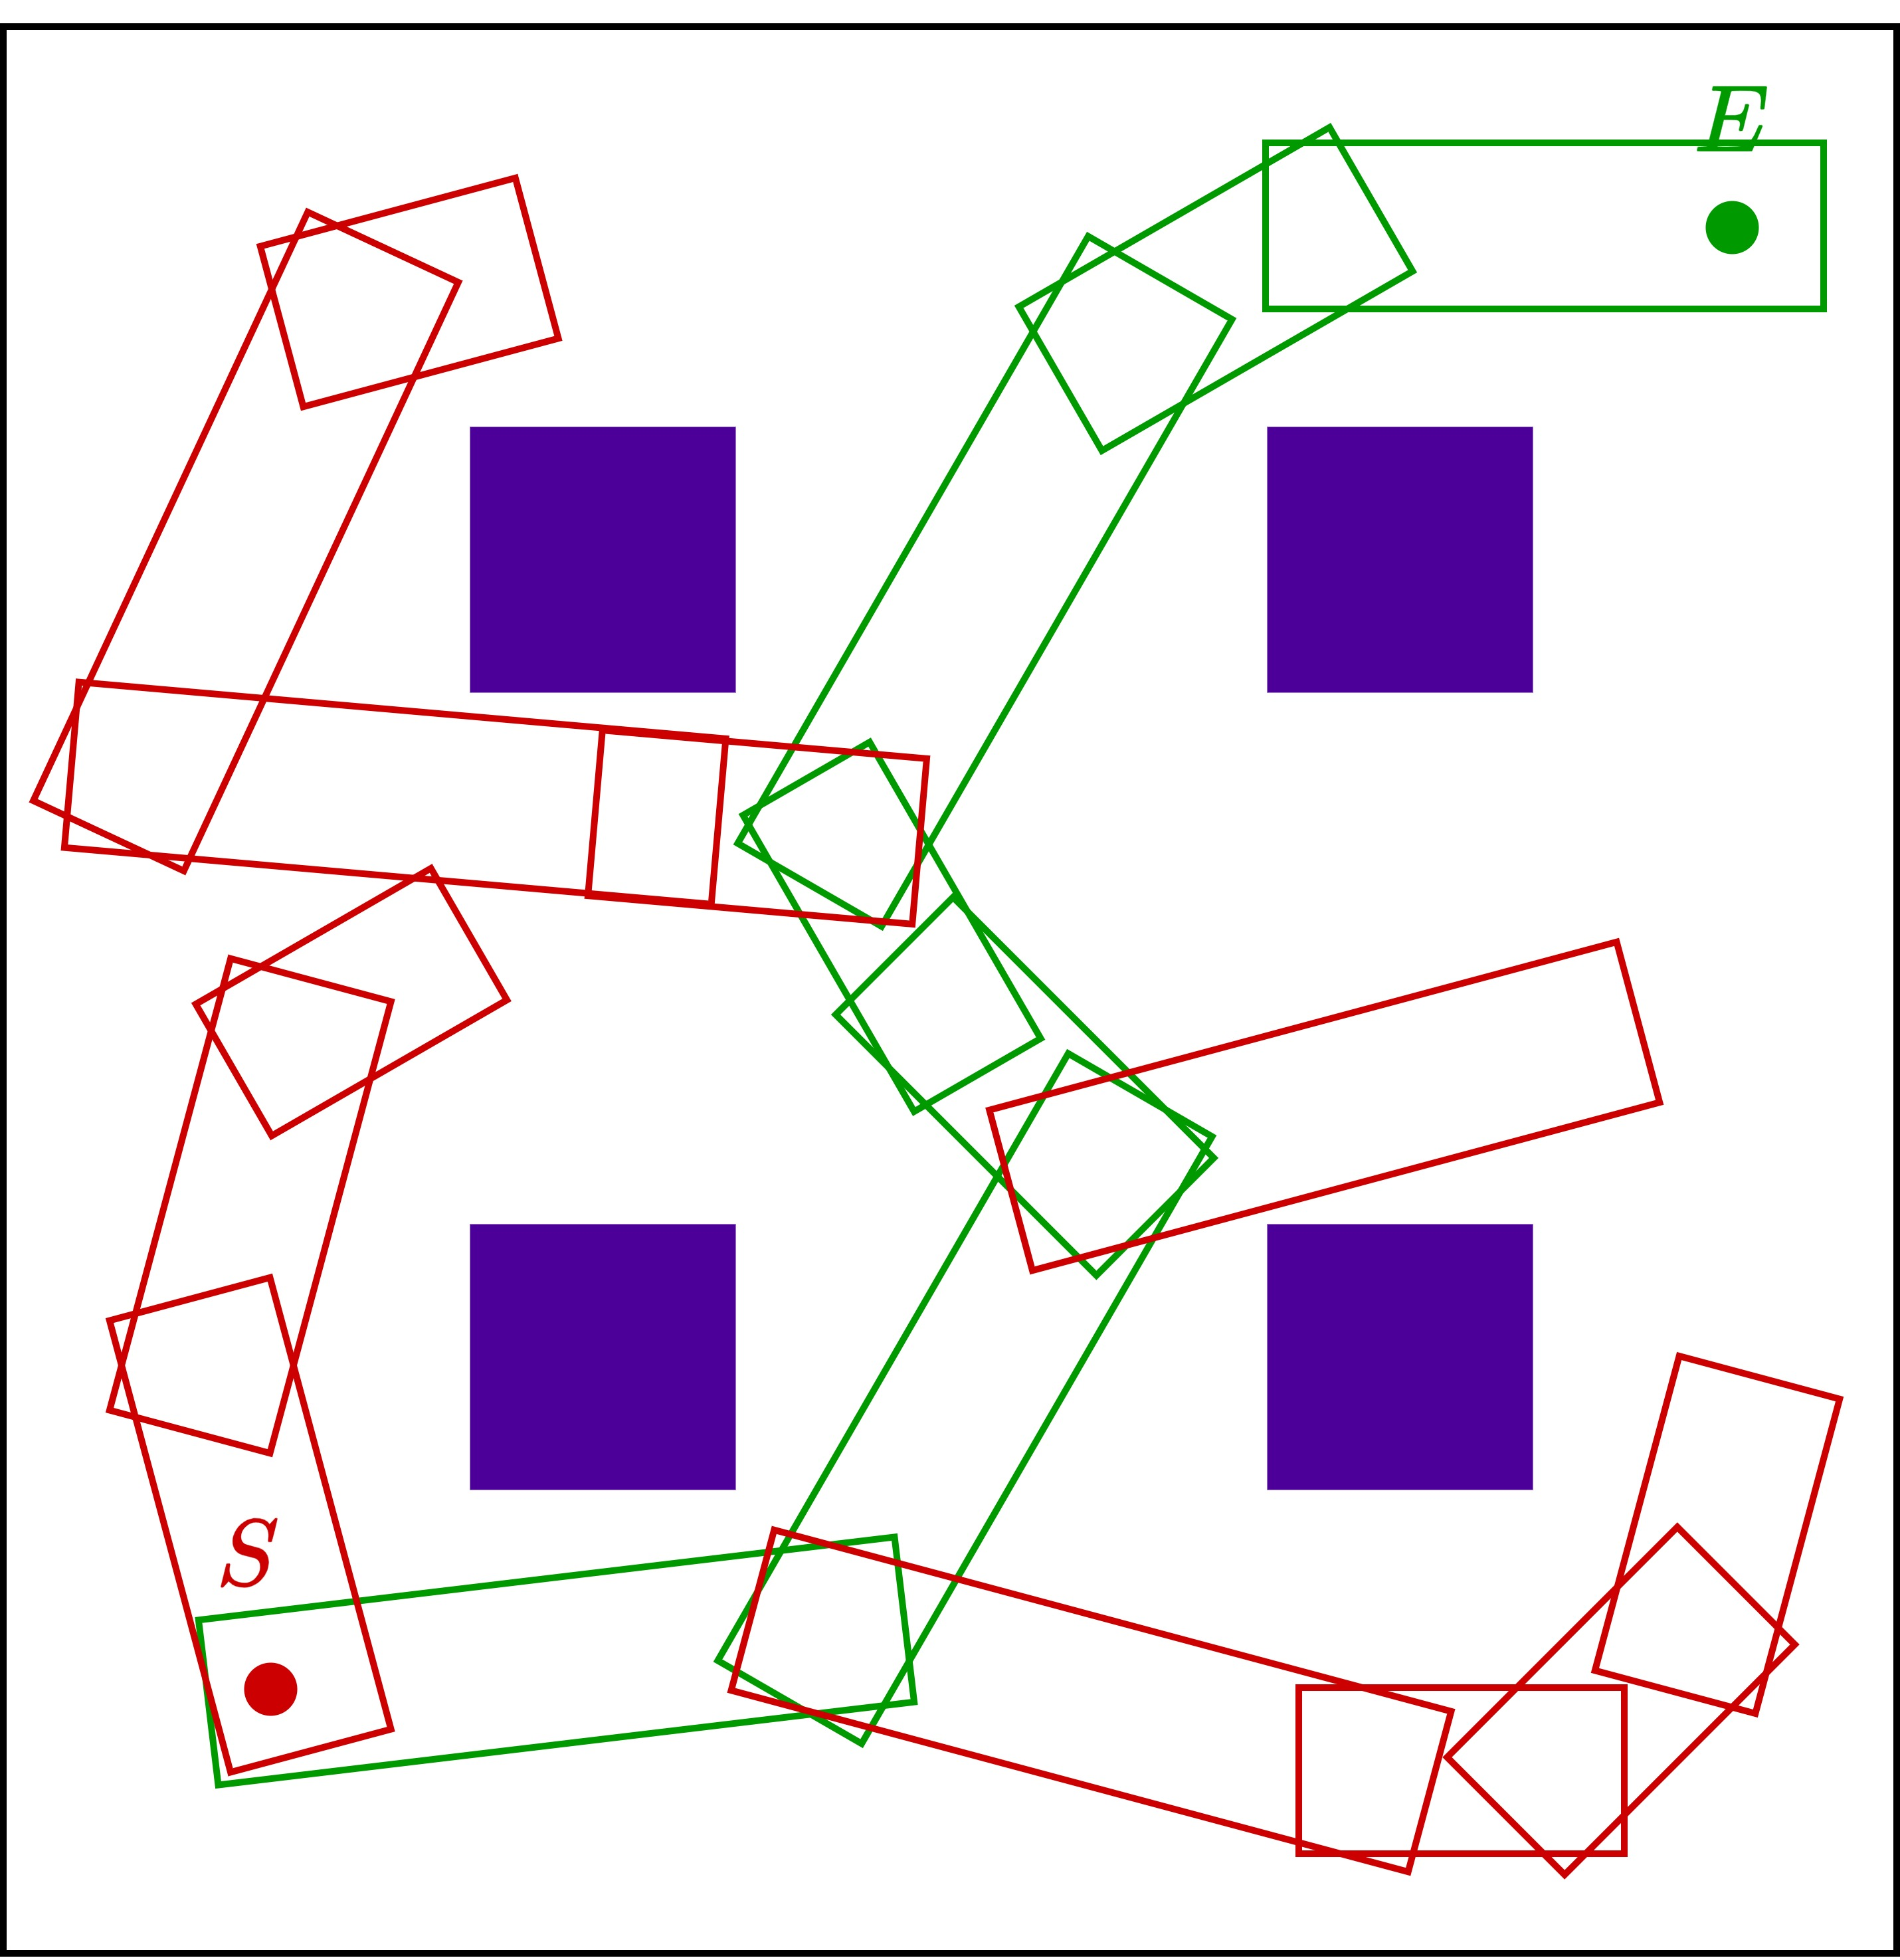
\includegraphics[width=0.9\linewidth]{figs/chap4/RRT Example Tree.jpg}
    \caption{SFC and obstacle intersections. On the left side, there is no intersection. On the right side there is an intersection.}
    \label{fig:obstacleIntersection}
\end{figure}

Each obstacle and each SFC is represented using its own linear constraint matrices. 
The obstacle has constraints $A_{obs}$ and $b_{obs}$, and the SFC has constraints $A_{sfc}$ and $b_{sfc}$. 
If there is an intersection, that means there is a feasible region such that both linear inequality constraints are met.
This is accomplished by concatenating both matrices as

\begin{align}
    A_{int} =
    \begin{bmatrix}
        A_{obs}\\
        A_{SFC}
    \end{bmatrix}
    \qquad
    b_{int} =
    \begin{bmatrix}
        b_{obs}\\
        b_{SFC}\\
    \end{bmatrix}
\end{align}.

This linear inequality is determined to be feasible or not using the Scipy linprog function.

\texttt{result = linprog(dummyVariable, Aub=Aint, bub=bint, bounds=tempBounds, method='highs')}

\texttt{intersectionOccurredTemp = result.success}

\section{Turn Constraints}
\label{sec:Turn Constraints}

Vehicle dynamic constraints impose limitations on the tree algorithm. 
Fixed-wing aircraft have a minimum turning radius, which is influenced by vehicle airspeed, thrust, and airframe design. 
Aircraft cannot physically turn with a smaller radius under such conditions. 
This fact is exploited for the formation of Dubins paths, which use only straight lines and circles of that minimum turning radius to get a very efficient and short path. 
Fixed-wing aircraft may not perform trajectories that have a tighter turn radius than a particular value, shown in Fig. \ref{fig:MinTurnRadius} .
For the Safe Flight Corridor tree, this imposes certain limitations on the possible geometries that can accommodate a particular minimum turning radius. 
This is depicted in figure \ref{fig:angular boundary conditions}.

\begin{figure}
    \centering
    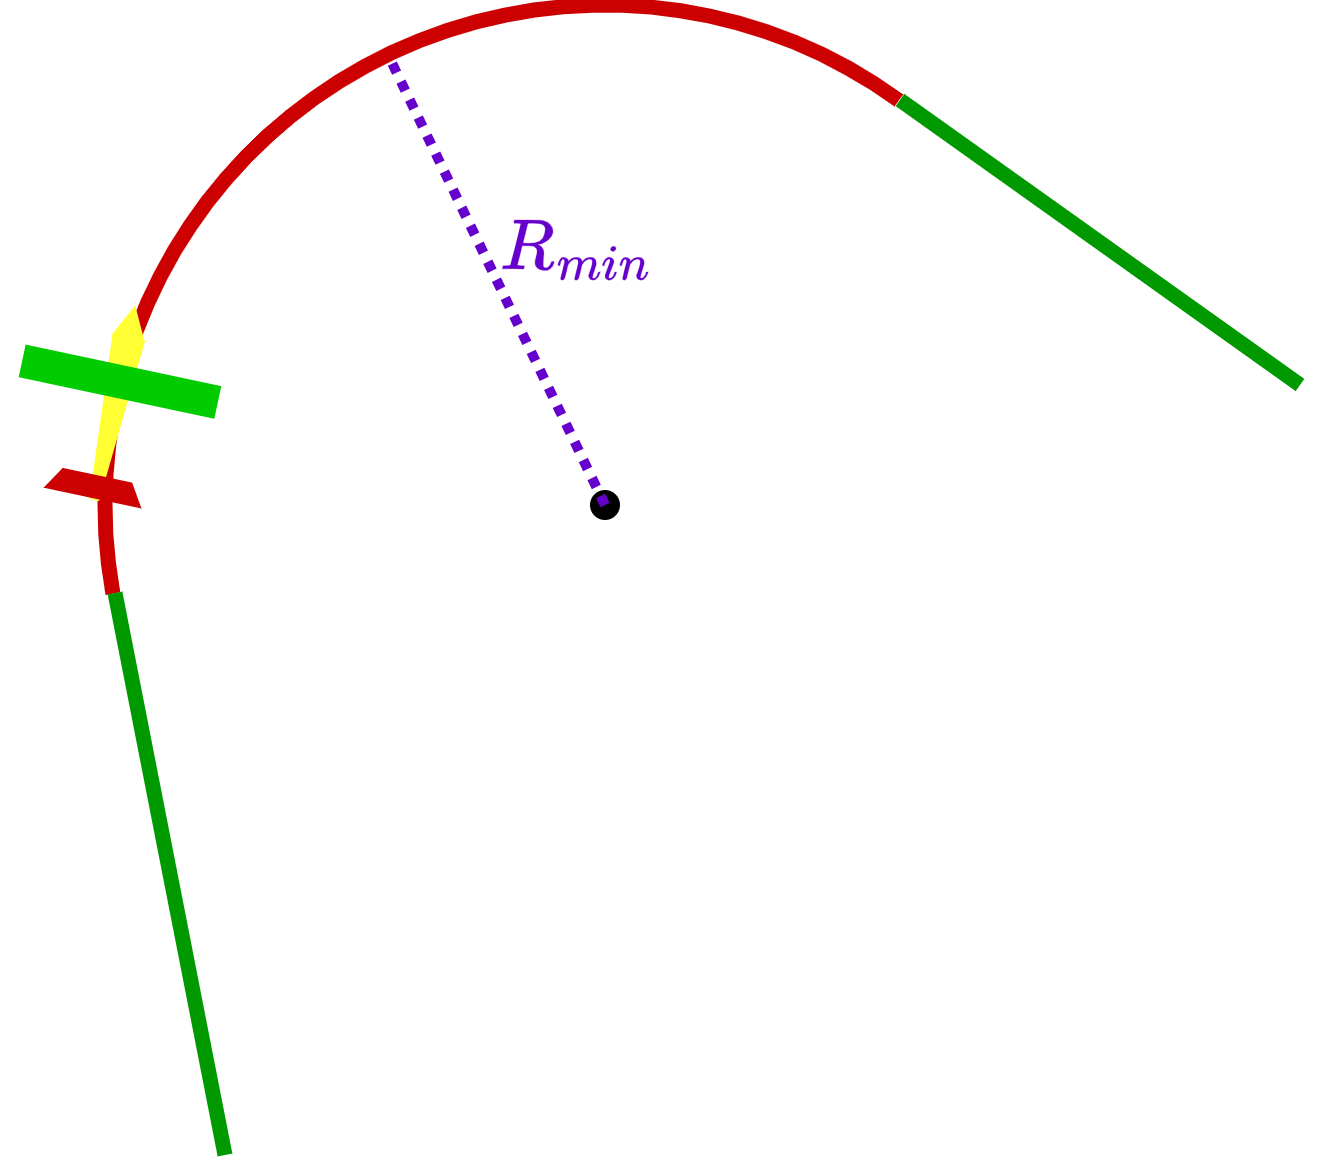
\includegraphics[width=0.5\linewidth]{figs/chap4/Minimum Turing Radius.drawio.png}
    \caption{Aircraft flying section of Dubins Path with straight lines, and connected with arcs of minimum turning radius. Anything with sharper curvature, and the aircraft will be unable to perform the turn.}
    \label{fig:MinTurnRadius}
\end{figure}

\begin{figure}
    \centering
    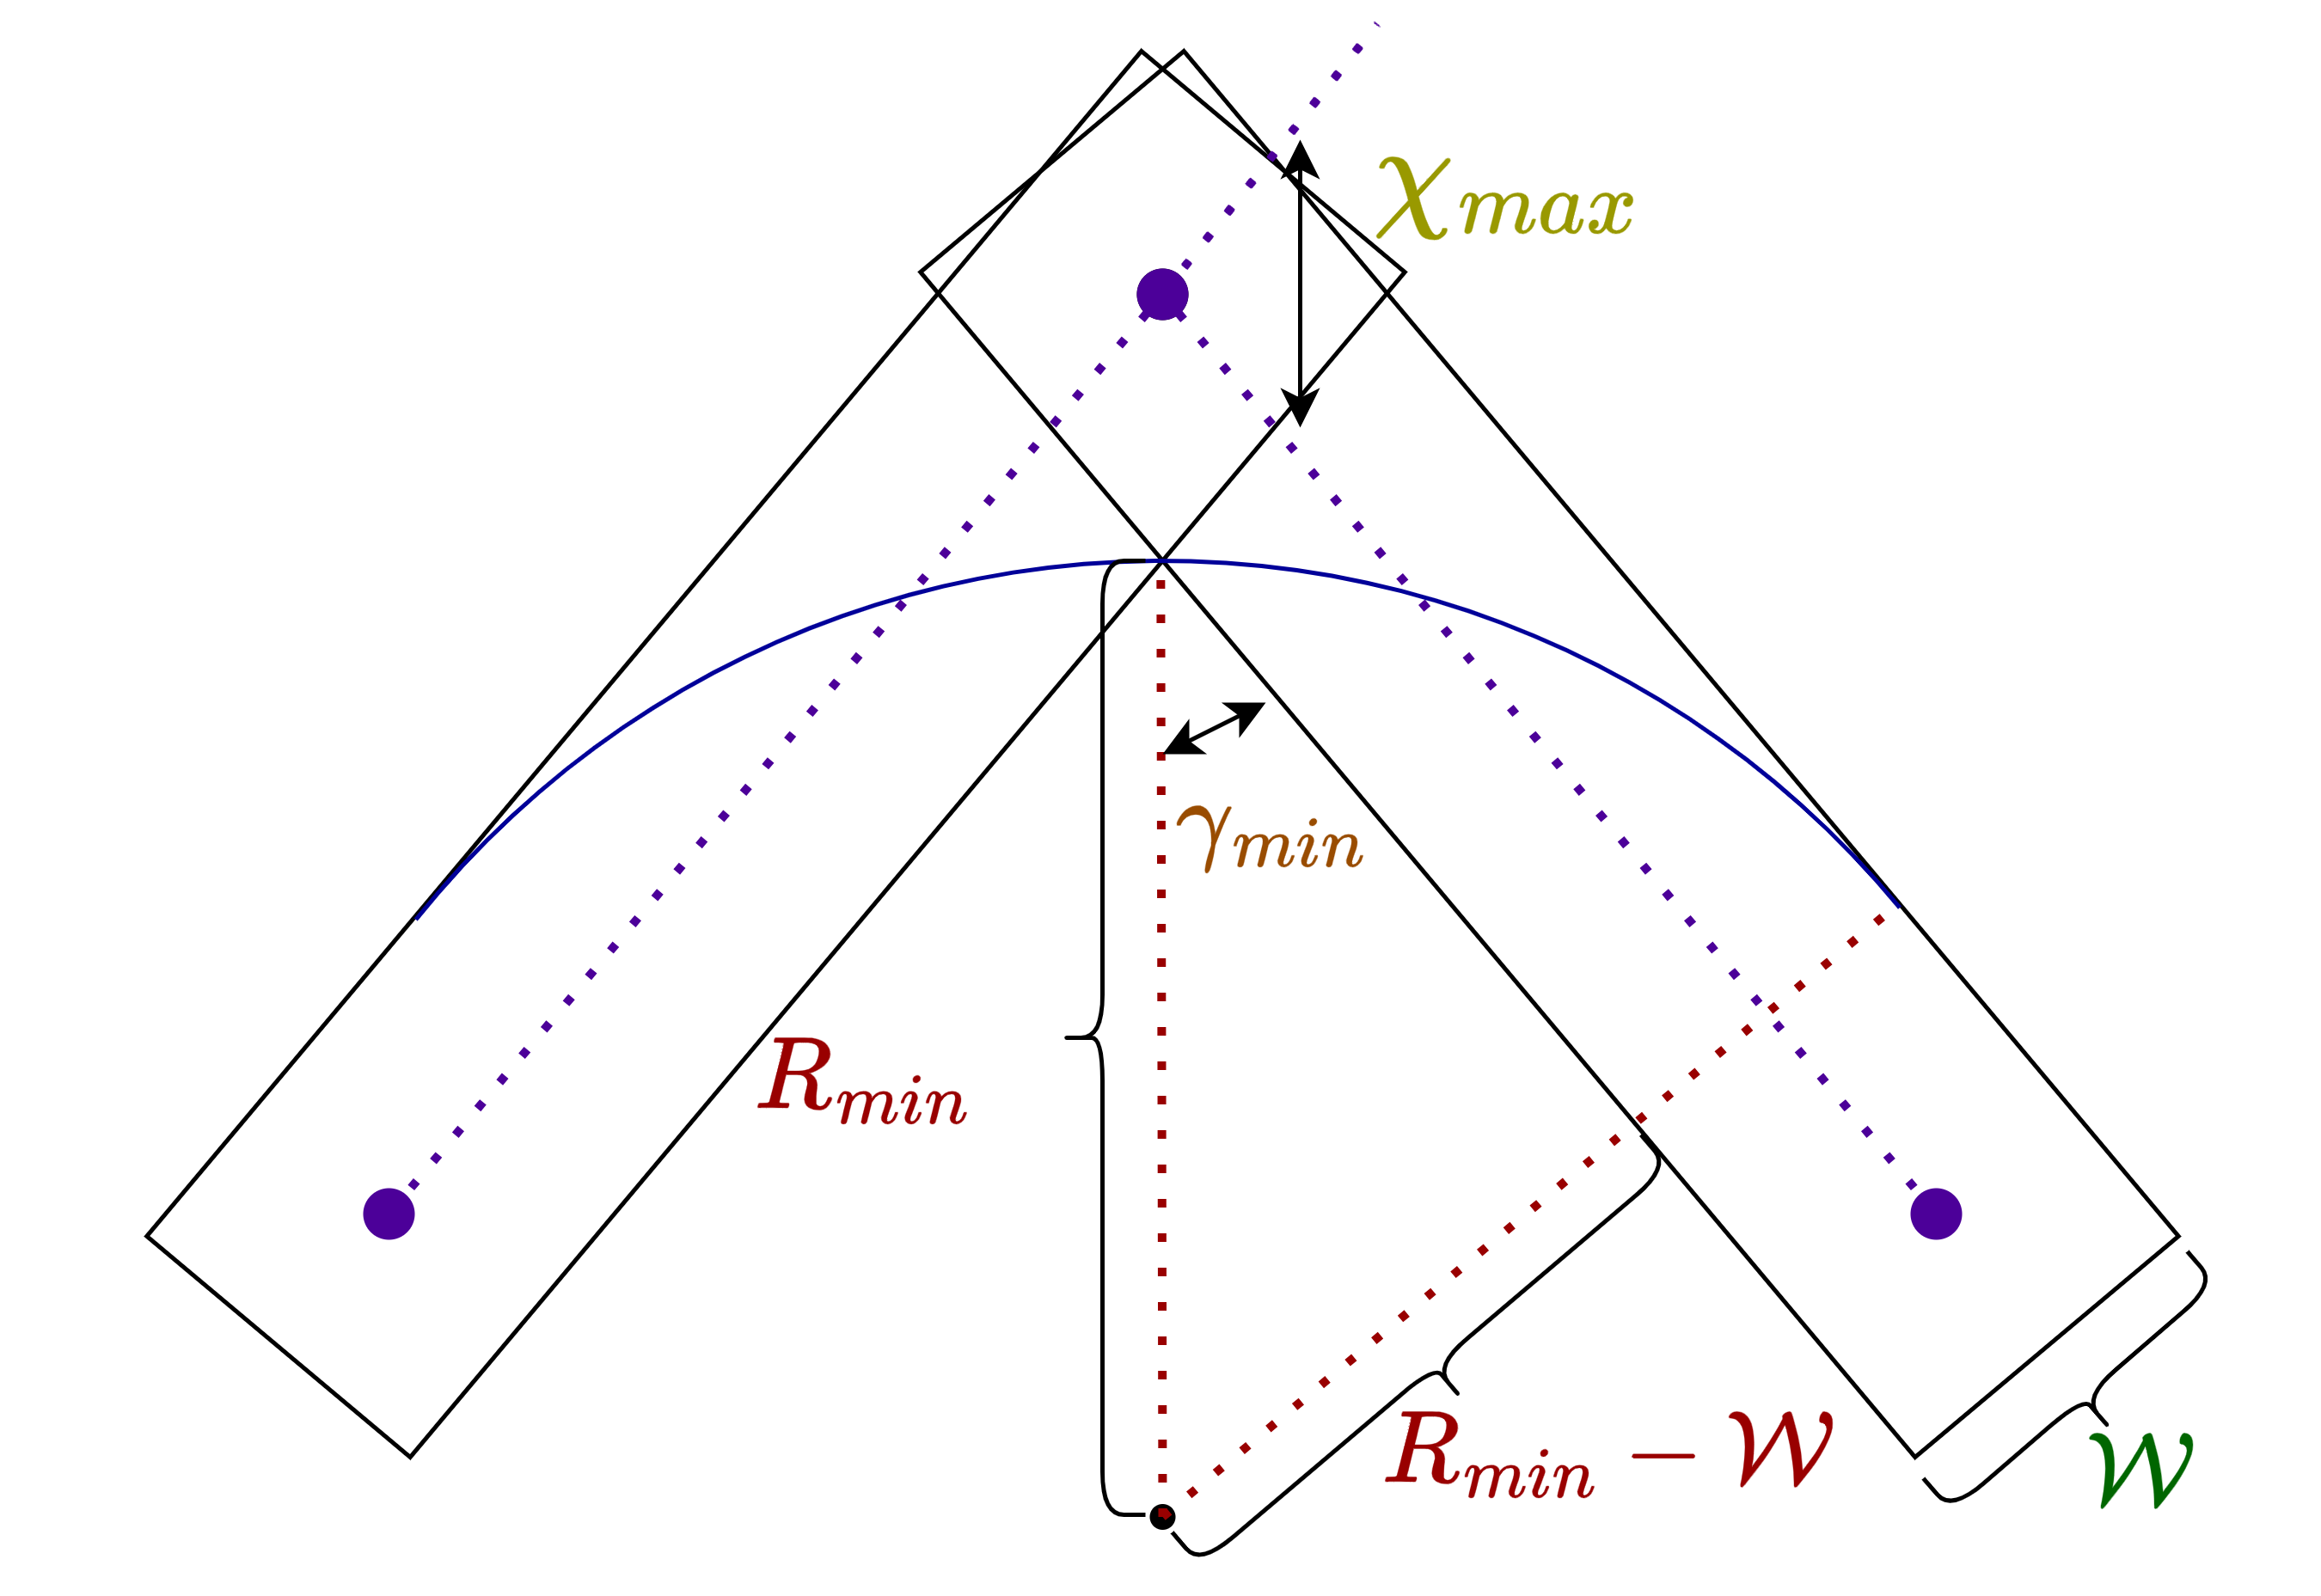
\includegraphics[width=0.5\linewidth]{figs/chap4/Turn Rate Constraints/SFC Angular Boundary Conditions (1).png}
    \caption{Turn rate constraint for Safe Flight Corridor intersection. This demonstrates the maximum turning angle between two SFCS using a superimposed circular flight path of the minimum allowable turning radius. If $\chi$ was any greater, the minimum turning radius would not be able to fit inside of the two safe flight corridors, and the aircraft's minimum turning radius would be violated.}
    \label{fig:angular boundary conditions}
\end{figure}


For a given minimum turning Radius $R_{min}$, the SFC boundary condition exists when the arc touches the inner corner of the SFC and the circle is tangent to the two outer walls. 
Under these conditions, the distance from the center point of the turn to the inner corner is $R_{min}$. 
The distance from the same center point is also $R_{min}$. 
However, because the arc is tangent to the outer wall, the radius line is perpendicular to the inner and outer wall on both sides. 
Therefore, the distance from the center to the inner wall is $R_{min} - \mathcal{W}$, where $\mathcal{W}$ is the SFC width.

From this geometry, a right triangle is formed with the inside area, where $\gamma_{min}$ represents the half angle between the two SFCs on the inside, and is defined as

\begin{align}
    \gamma_{min} = \arcsin{\frac{R_{min} - \mathcal{W}}{R_{min}}}
\end{align}.

This triangle is a similar triangle to the one touching the center chord, and has the same angular relationships. 
Therefore, $\chi_{max}$, the outside angle between two SFCs is defined as

\begin{align*}
    \chi_{max} = \pi - 2 \cdot \gamma_{min}\\
    \chi_{max} = \pi - 2 \cdot \arcsin{\frac{R_{min} - \mathcal{W}}{R_{min}}}\\
\end{align*}.

For example, if $\mathcal{W} = 30$ and $R_{min} = 100$, then $\chi_{max} = 1.591 = 91.146^\circ$.

During the RRT phase of the algorithm, the actual angle between $SFC_{i-1}$ and $SFC_i$ is calculated as $\chi_{act}$. 
If a candidate $SFC_i$ is found which violates this such that $\chi_{act} > \chi_{max}$, then this candidate $SFC$ is omitted and the process is repeated until an SFC with $\chi_{act} \leq \chi_{max}$ is found.

\subsection{Turn Constraints Enforcement}

In order to enforce this minimum turn radius constraint, or at least to minimize its violation, constraints must be enforced upon the control points in the intersection region.
While a circle or section of a circle is convex, the area between two concentric circles is not. 
This shape, also known as an annulus is shown in Fig. \ref{fig:annulus concentric circle}.

\begin{figure}
    \centering
    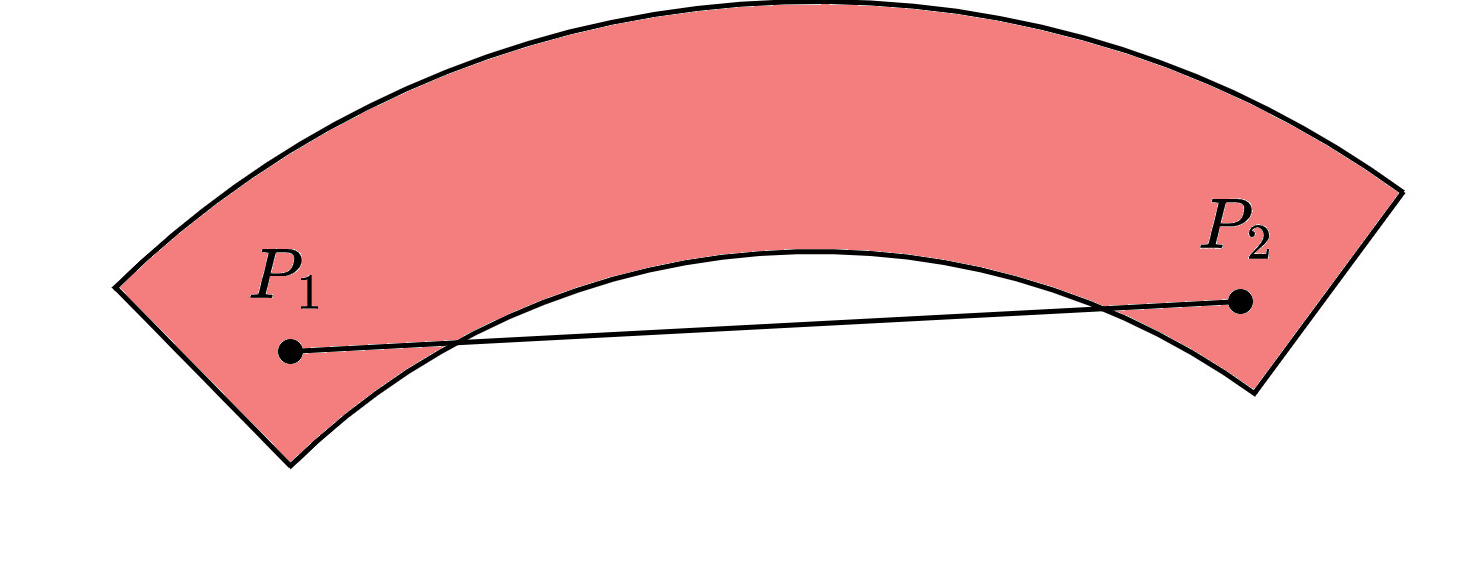
\includegraphics[width=0.5\linewidth]{figs/chap4/Turn Rate Constraints/Annulus Concentric Circles.jpg}
    \caption{Arc section of two concentric circles, called an annulus. The line from $P_1$ to $P_2$ demonstrates this is a non-convex region.}
    \label{fig:annulus concentric circle}
\end{figure}

Fortunately, constraints may be made on the control points by approximating the annulus. 
By sampling the points along the minimum turning radius, along with an outer radius, an approximation can be made for the inner turning radius. 
This provides a convex hull for the control points. 
One control point will be constrained to a single annulus approximation section, as shown in figure \ref{fig:annulus sampled diagram}. 
These sections will be termed annulus segments. 

\begin{figure}
    \centering
    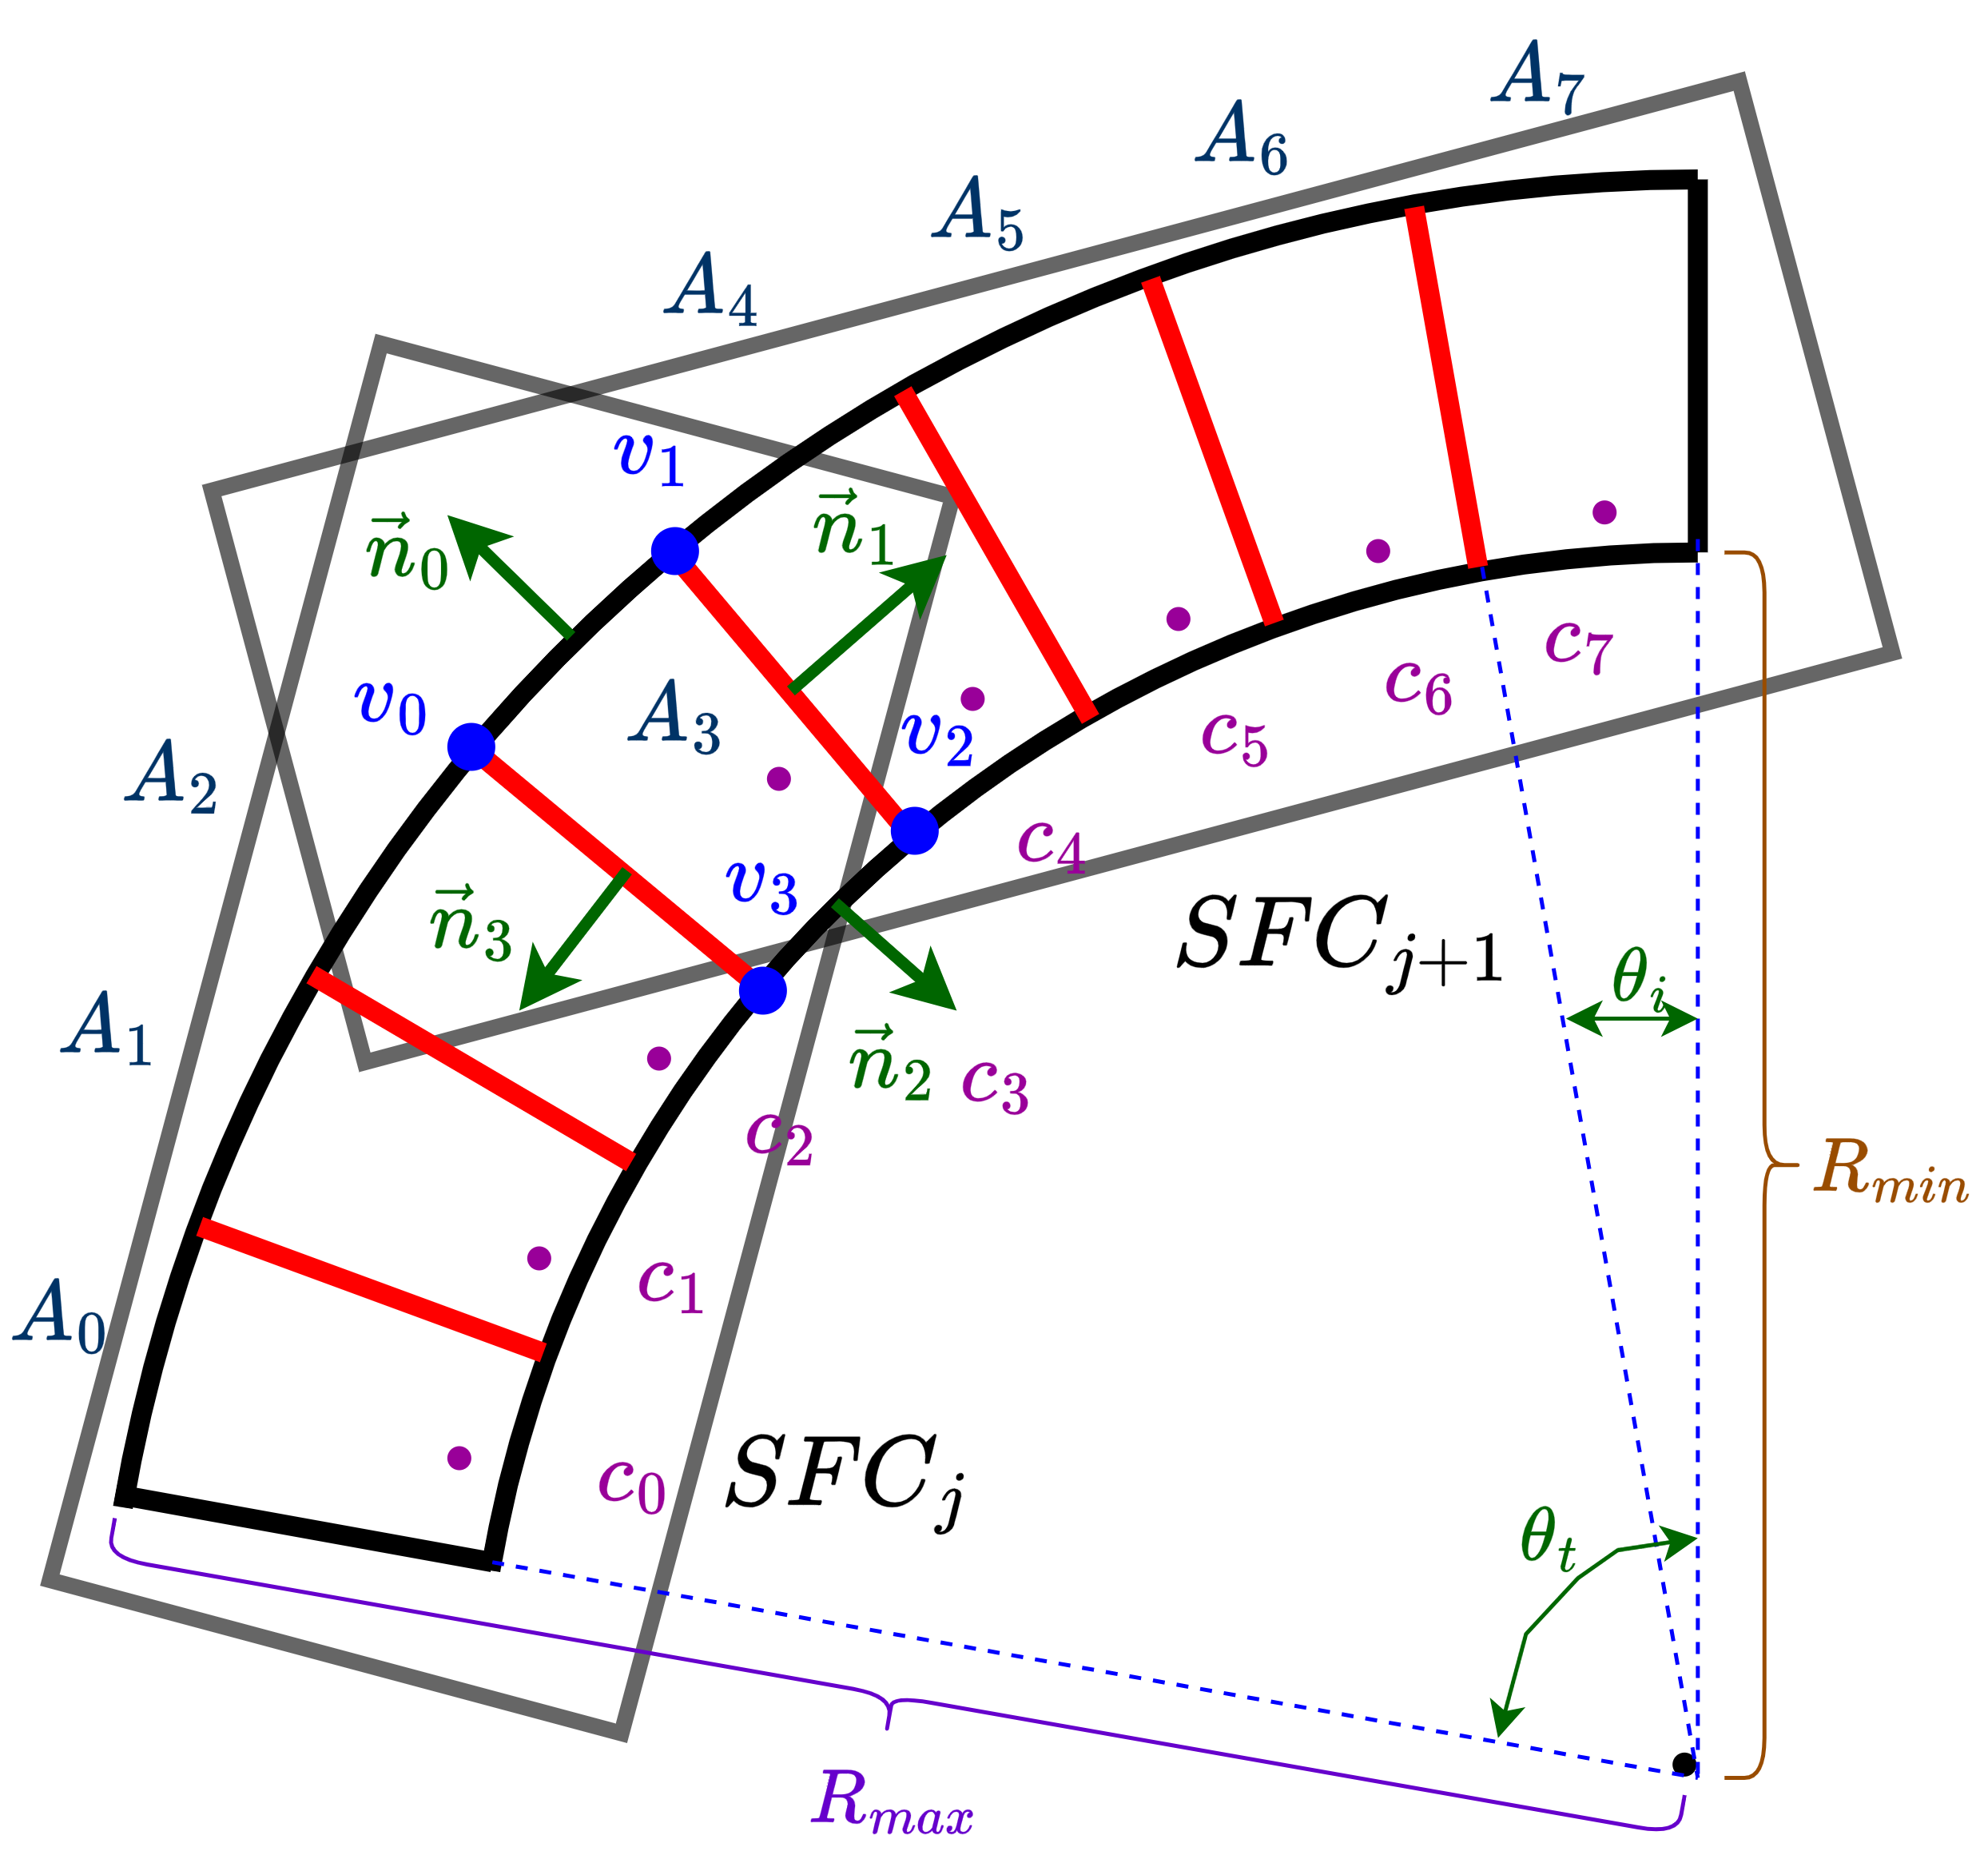
\includegraphics[width=0.5\linewidth]{figs/chap4/Turn Rate Constraints/Annulus diagram (1).png}
    \caption{Diagram of sampled annulus constraints}
    \label{fig:annulus sampled diagram}
\end{figure}

As with safe flight corridors, control points may be constrained within annulus segments using the matrix form $Ax \leq b$.

\section{Path Smoothing}

The initially generated path produces suboptimal results for an SFC path; the segments are short and take a random path, as there is not an RRT* smoothing operation for reasons of computational efficiency. 
To solve this problem, we implemented a variation of Dijkstra's algorithm to smooth an initial path.

\begin{figure}
     \centering
     \begin{subfigure}[b]{0.45\textwidth}
         \centering
         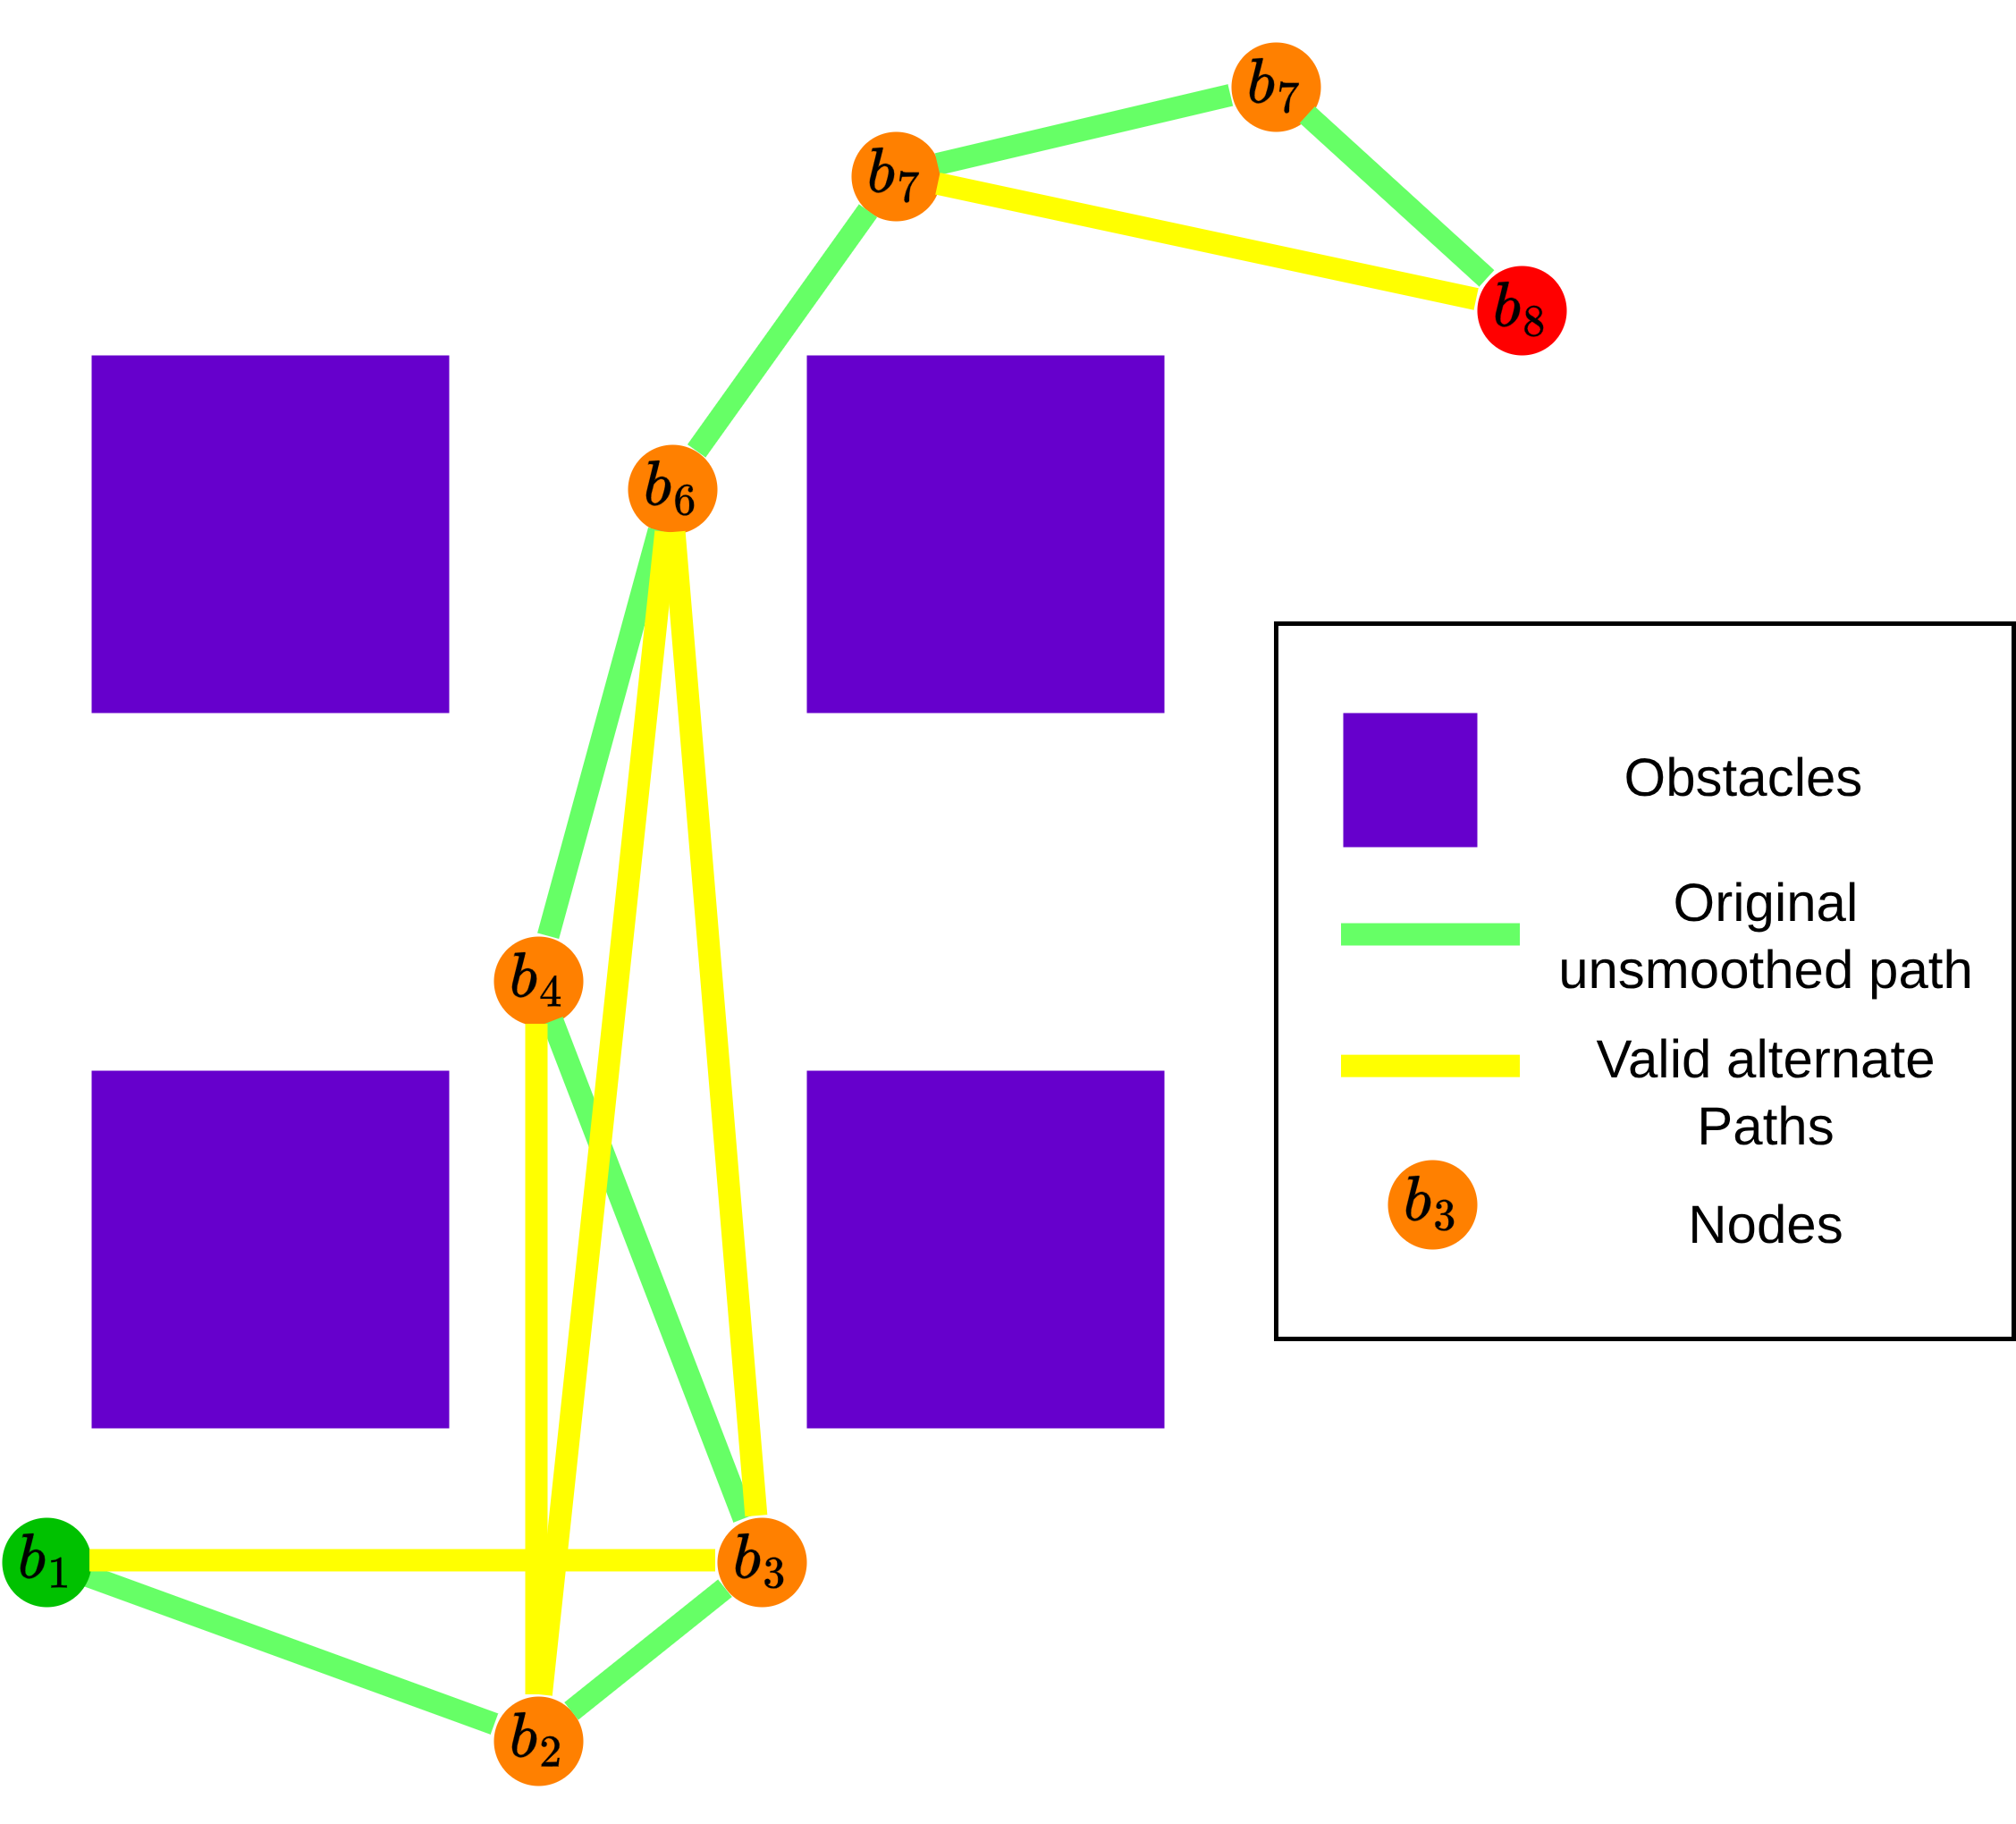
\includegraphics[width=\textwidth]{figs/chap4/Smoothing/Dijkstra's Possibilities.drawio.png}
         \caption{Complete set of nodes for RRT algorithm on a $2 \times 2$ obstacle field. The intermediate nodes are shown in orange and the original path is shown in green connecting them sequentially. The other plausible paths between existing nodes are shown in yellow. These alternative paths will be explored using Dijkstra's algorithm.}
         \label{fig:blank 3D obstacle field}
     \end{subfigure}
     \hfill
     \begin{subfigure}[b]{0.45\textwidth}
         \centering
         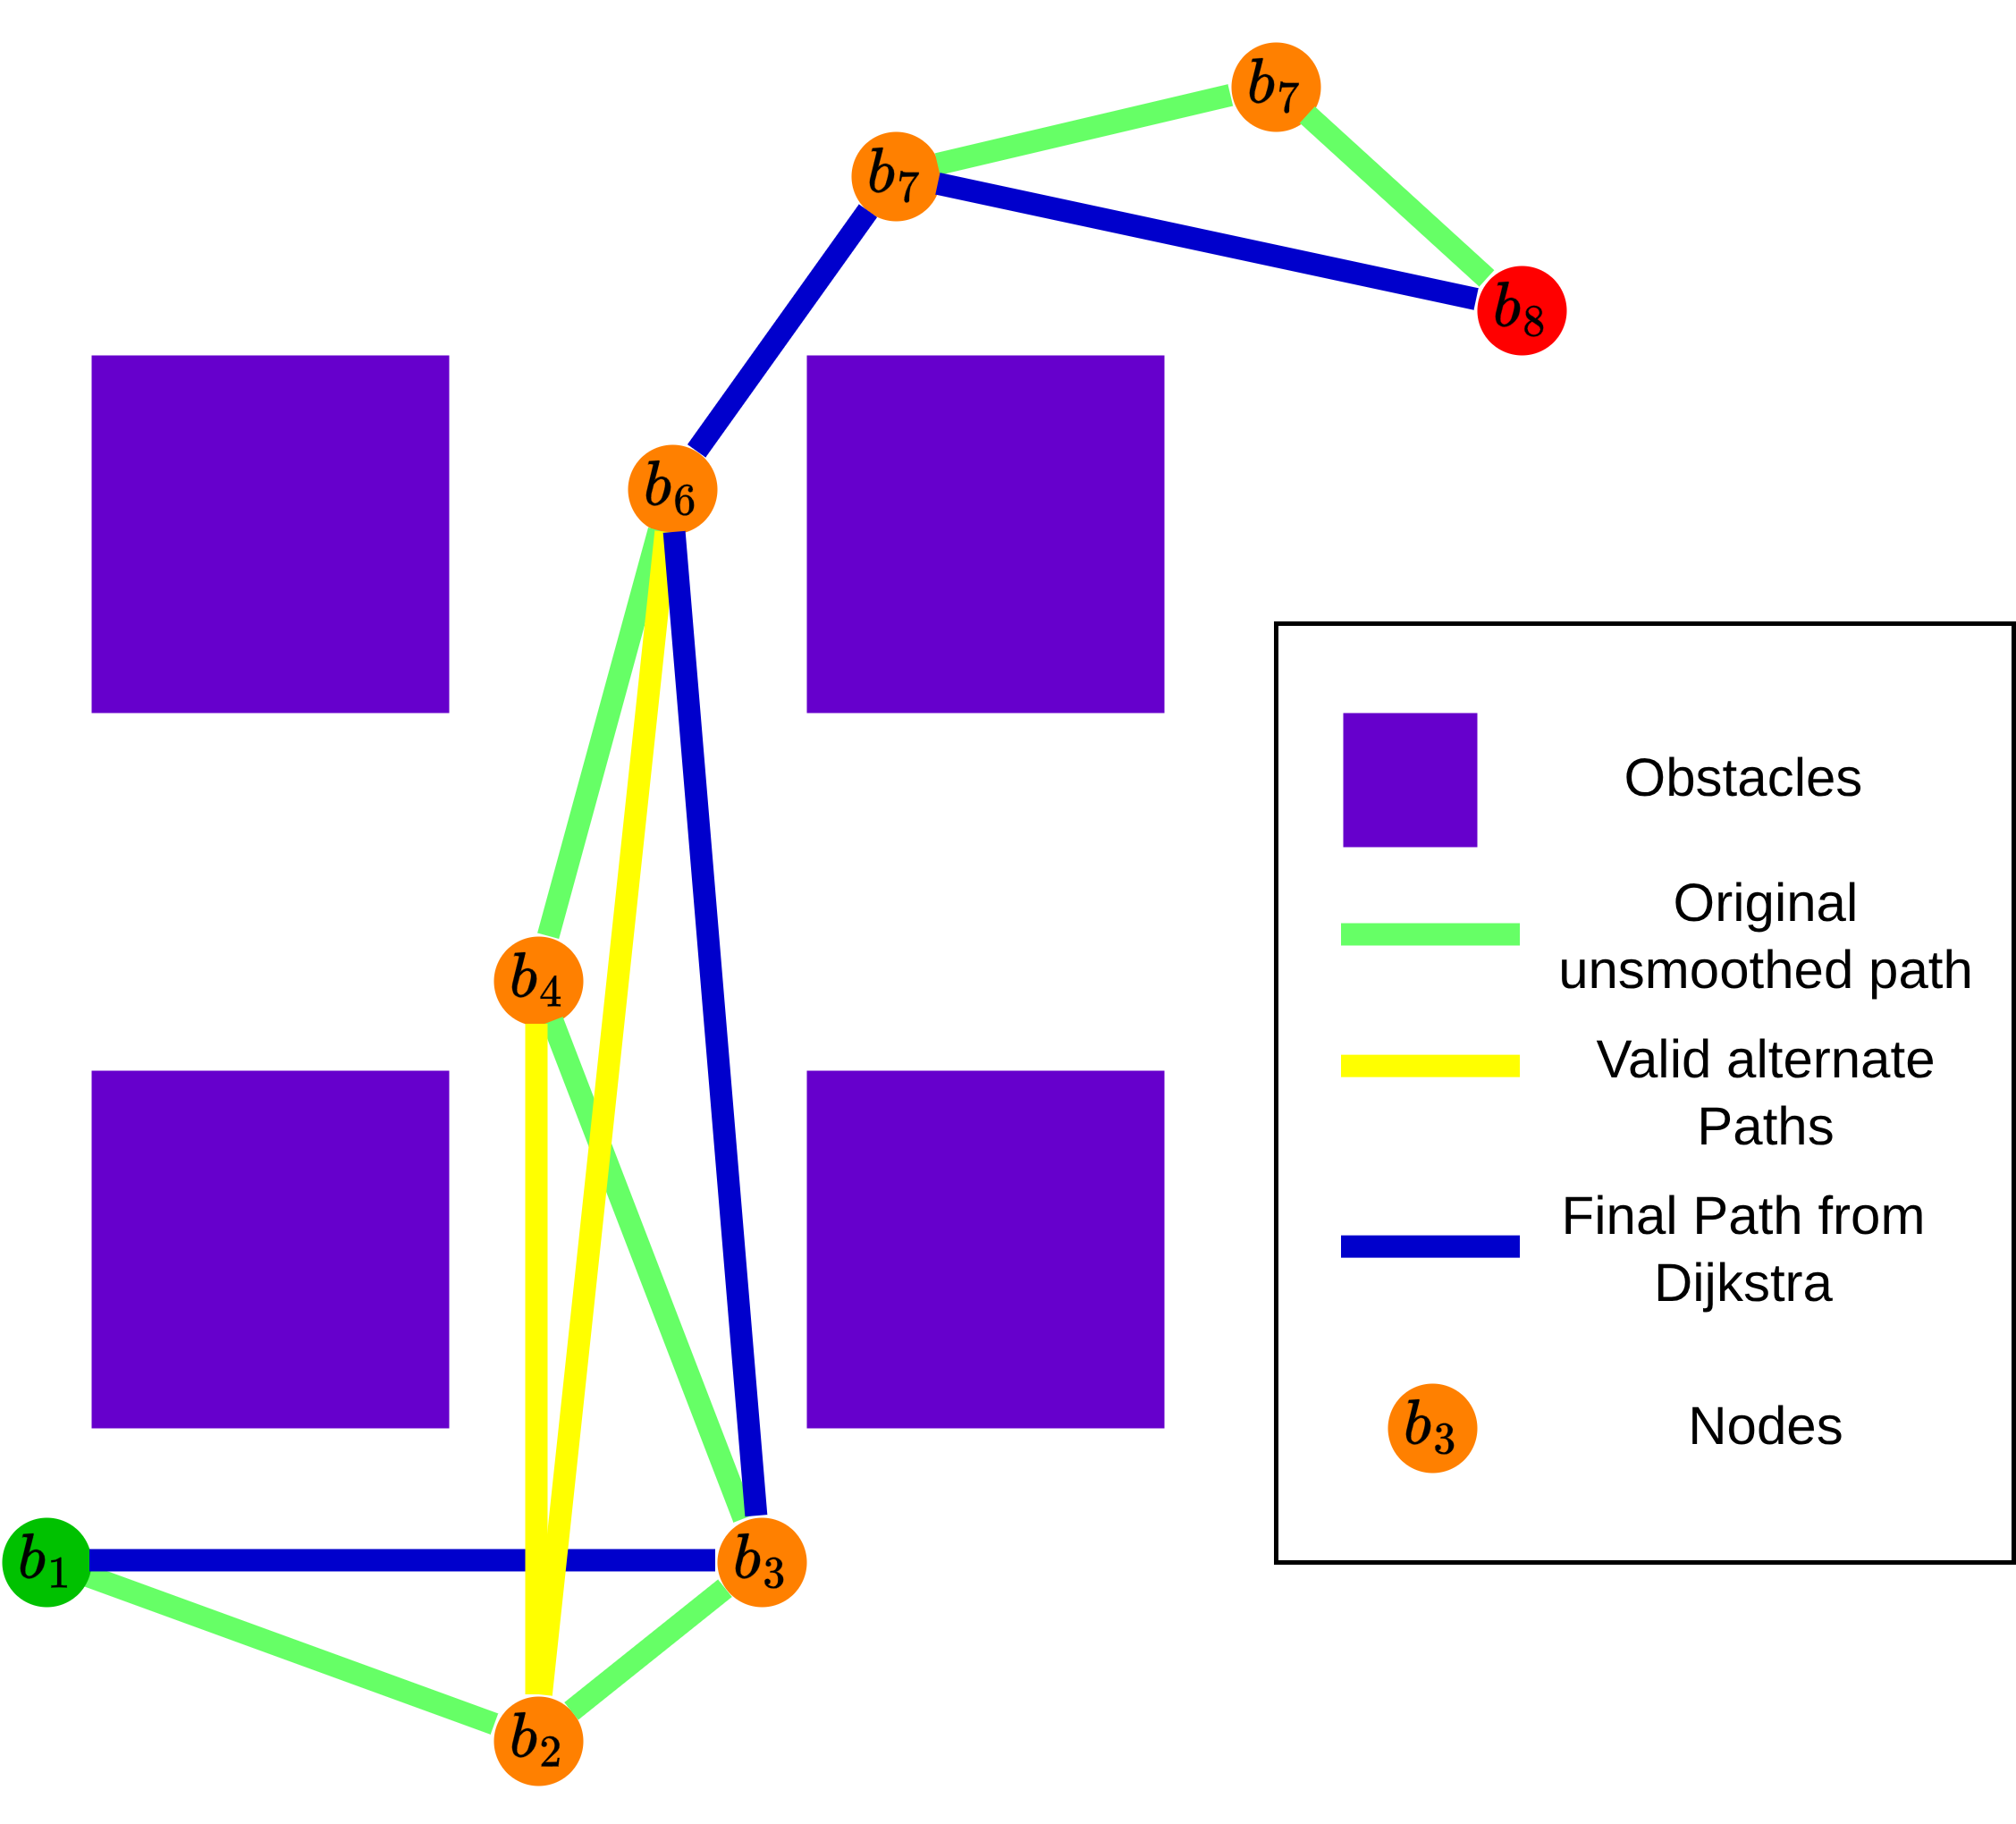
\includegraphics[width=\textwidth]{figs/chap4/Smoothing/Dijkstra's Smoothed.drawio.png}
         \caption{This displays the same node network, but with Dijkstra's algorithm outputting smoothed path in blue}
         \label{fig:3D Waypoints Not Smooth}
     \end{subfigure}

    \caption{Diagram of initial RRT output and all possible alternative connections between nodes. Dijkstra's algorithm finds the shortest possible route in the end.}
    \label{fig:3D Path}
\end{figure}

Dijkstra's algorithm finds the shortest path between two connected nodes over a field of connected nodes, with an associated cost or distance for each connection. 
An explanation for the actual algorithm is found in the original paper by Edsger Dijkstra from 1959 in \cite{EWD:NumerMath59}. 
The method of using Dijkstra's algorithm may be seen in Fig. \ref{fig:3D Path}.

\section{Objective Function}

It is desirable to optimize the performance of the B-Spline by finding the best possible curve given the safe flight corridor constraints. 
The first step is to find a cost or penalty associated with a particular configuration of control points. 
There must be a mathematical relationship between a particular configuration of the control points and some sort of cost so that adjusting the position of the control points minimizes the cost. The simplest metric is to minimize the length of the B-Spline for the shortest possible path from start to finish. 

Fortunately, there is a direct mathematical relationship between the placement of the control points and the maximum length, velocity, and acceleration of the spline. 
The objective functions for maximum position, velocity, and acceleration are given in \textit{\citetitle{beard2025BSplines}} \cite{beard2025BSplines} in sections 2.2, 2.3, and 2.4 respectively. 

\subsection{Minimum Distance}

The length of a B-Spline on the interval $t\in[s,s+1]$ is given by:

\begin{align}
    \min_{m\in[s+1,s+d]}\norm{\bs{c}_m-\bs{c}_{m-1}} \leq L \leq \sum_{m=s+1}^{s+d}\norm{\bs{c}_m-\bs{c}_{m-1}}
\end{align}

The term $\bs{c}_m-\bs{c}_{m-1}$ refers to the vector from one control point to the next, which is the equivalent velocity control point. 
This can also be expressed as $\bs{c}^v_{m-1} = \bs{c}^p_m - \bs{c}^p_{m-1}$. 

\begin{figure}
    \centering
    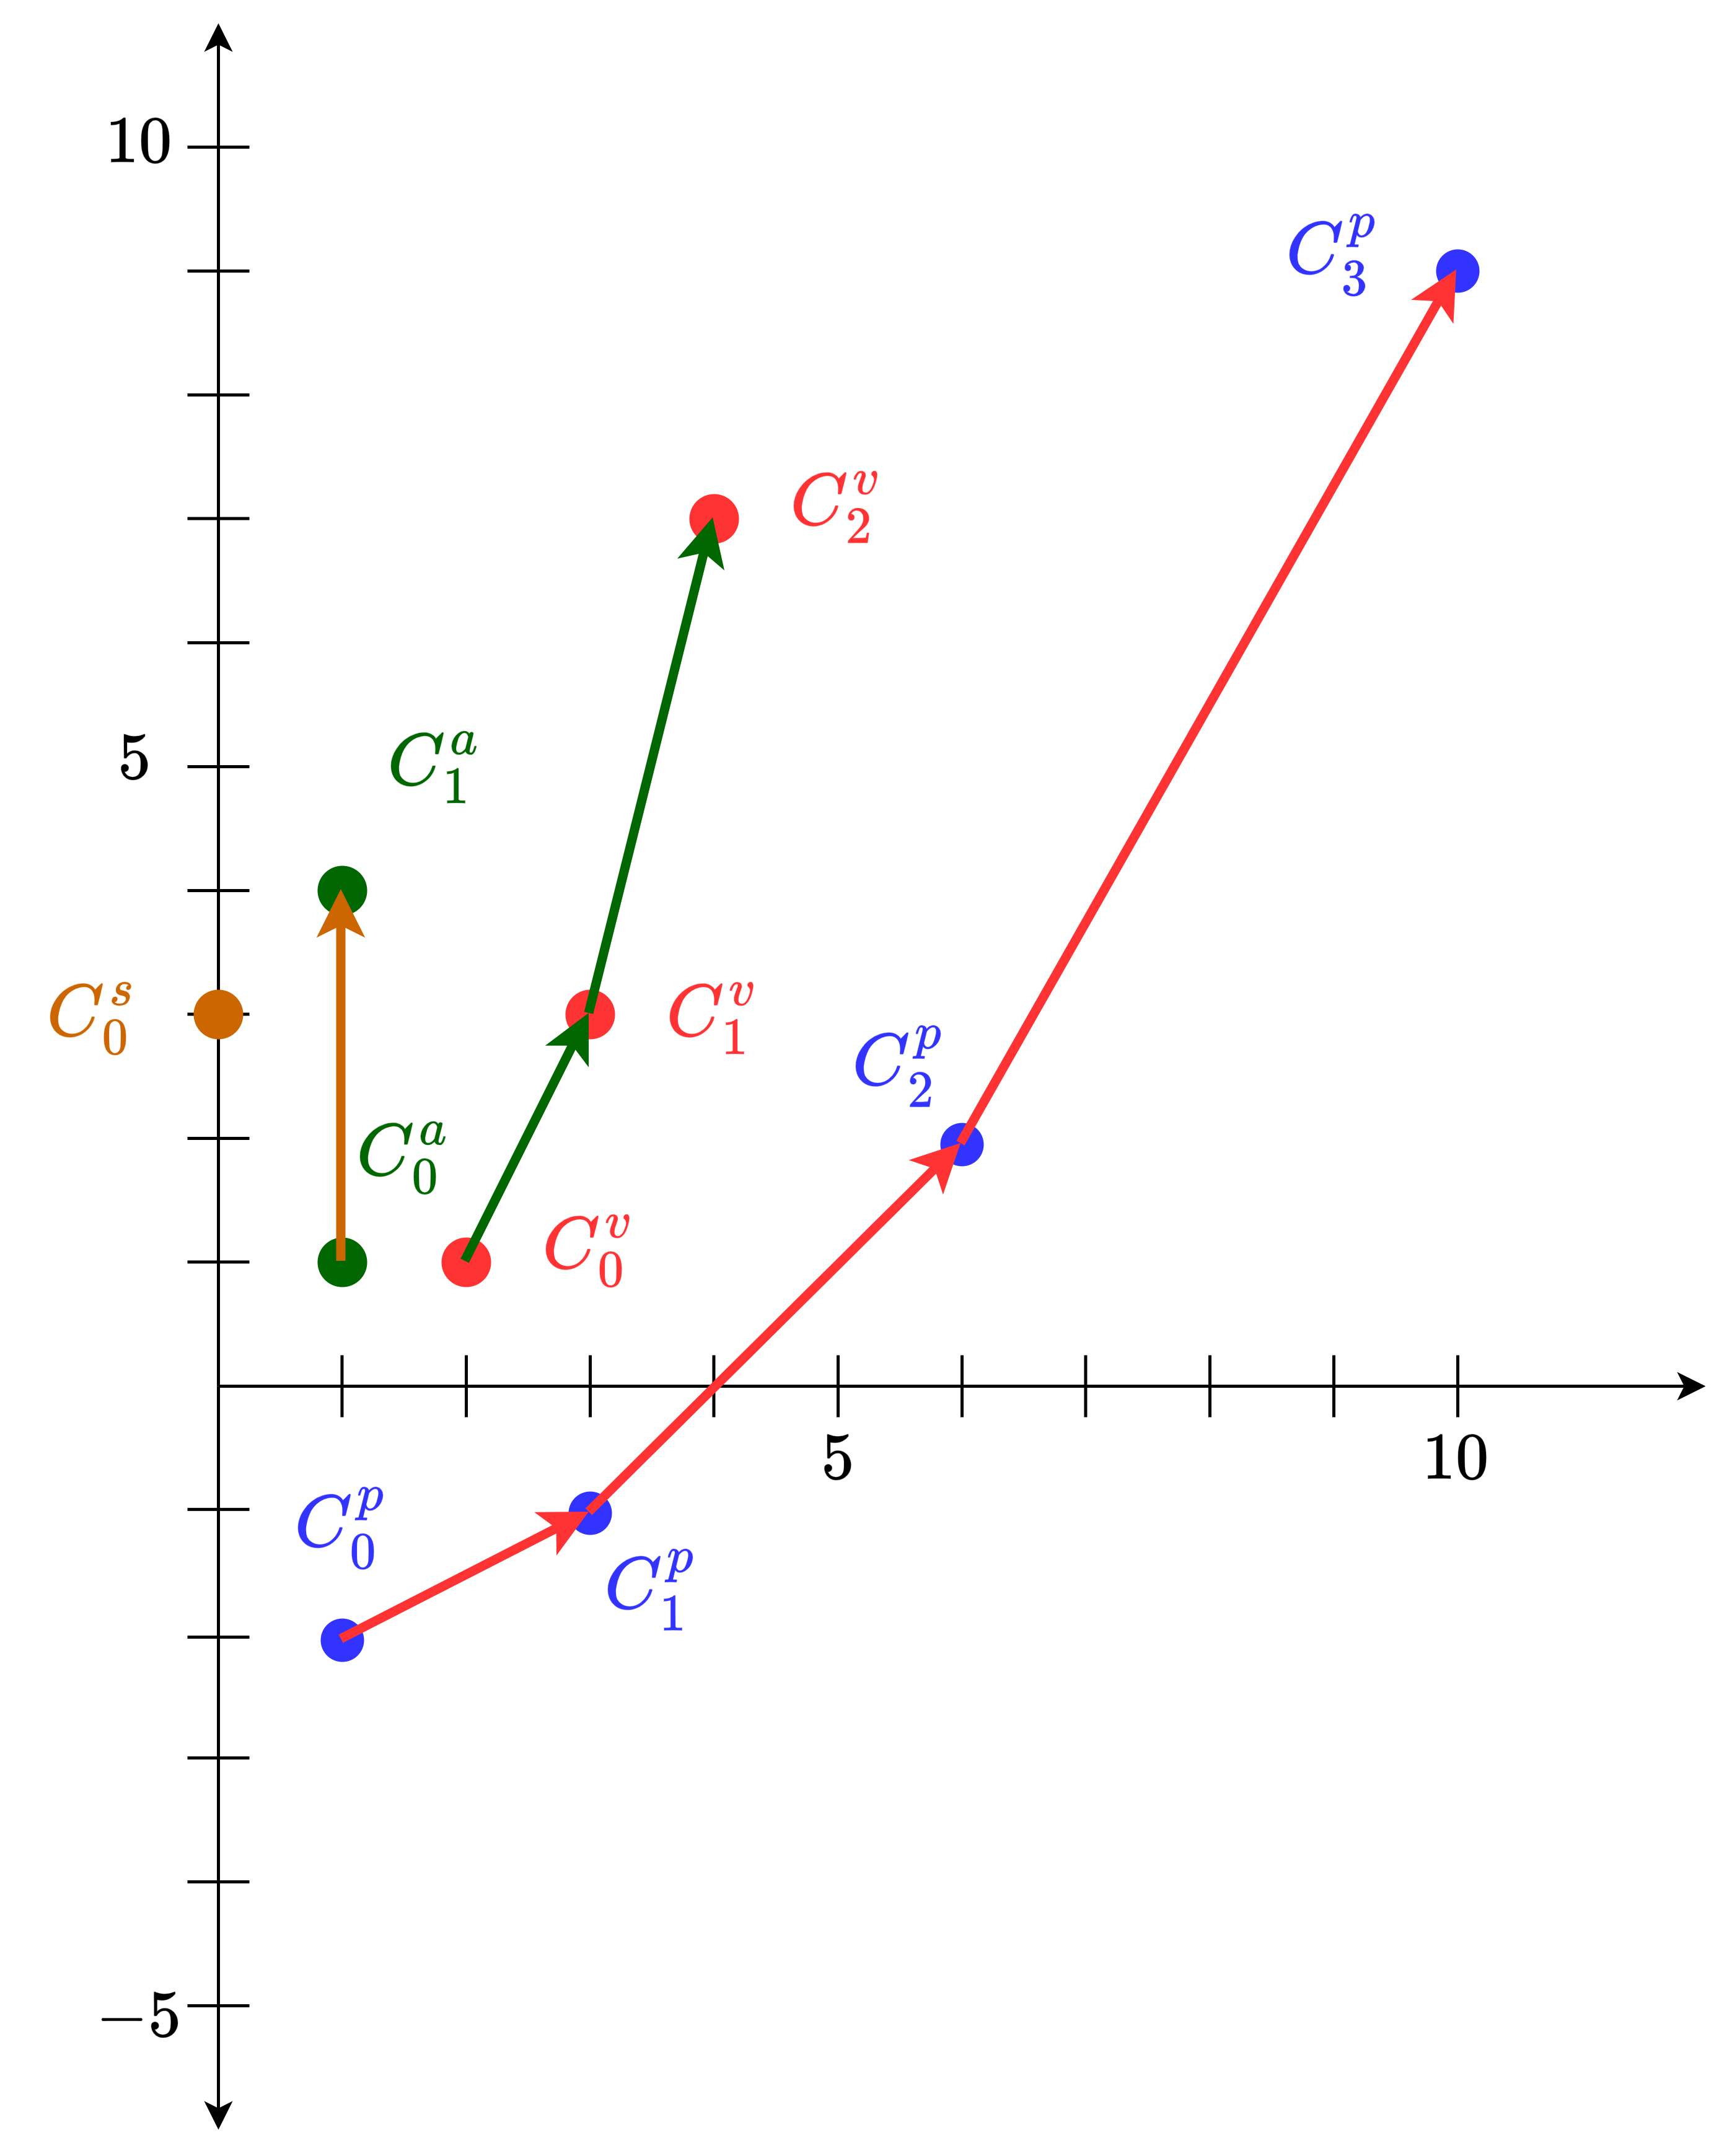
\includegraphics[width=0.5\linewidth]{figs/chap4/Control Points Relationship.drawio.png}
    \caption{Diagram of relationships between Control Points. This example shows that the vectors between control points are the control points of the derivative.}
    \label{fig:Control Points Relationships}
\end{figure}

\begin{align}
    V = C_{0:N-2} - C_{1:N-1}\\
    D_{max} = 
    \sum_{i=0}^{N-1} |V(i)|\\
\end{align}

The minimum distance optimization function then becomes

\begin{equation}\label{eq:controlPointsOptimizationDistance}
    \begin{aligned}
        &\text{minimize} && \sum_{k=0}^{N-1} \|C_{0:N-2}(k) - C_{1:N-2}(k)\|\\
        &\text{with respect to} && C_{pts}\\
        &\text{subject to} && A_{tot} C_{pts} < b_{tot}\\
        &&& C_{1:d} = S \hat{B}_M^d(0)^{-1}\\
        &&& C_{(M+1):(M+d)} = E \hat{B}_M^d(0)^{-1}\\
    \end{aligned}
\end{equation}.

\subsection{Minimum Velocity}

Minimum distance is not the only possible objective function. 
As the sum of velocity control points represents an upper limit on the total distance of the B-Spline, the sum of acceleration control points represents an upper limit on a velocity metric for the resulting B-Spline. 
This is given as

\begin{align}
    A = C_{0:N-3} + C_{2:N-1} - 2 \cdot C_{1:N-2}\\
    V_{max} = 
    \sum_{i=0}^{N-2} |A(i)|\\
\end{align}.

The minimum velocity optimization function then becomes

\begin{equation}\label{eq:controlPointsOptimizationVelocity}
    \begin{aligned}
        &\text{minimize} && \sum_{k=0}^{N-2} \|C_{0:N-3}(k) + C_{2:N-1}(k) - 2 C_{1:N-2}(k)\|\\
        &\text{with respect to} && C_{pts}\\
        &\text{subject to} && A_{tot} C_{pts} < b_{tot}\\
        &&& C_{1:d} = S \hat{B}_M^d(0)^{-1}\\
        &&& C_{(M+1):(M+d)} = E \hat{B}_M^d(0)^{-1}\\
    \end{aligned}
\end{equation}.

\subsection{Minimum Acceleration}

Likewise, an acceleration objective function may also be minimized using the jerk control points as

\begin{align}
    J = C_{3:N-1} - 3 \cdot C_{2:N-2} + 3 \cdot C_{1:N-3} - C_{0:N-4}\\
    A_{max} = 
    \sum_{i=0}^{N-3} |J(i)|\\
\end{align}.

The minimum acceleration optimization function then becomes

\begin{equation}\label{eq:controlPointsOptimization}
    \begin{aligned}
        &\text{minimize} && \sum_{k=0}^{N-2} \|C_{3:N-1}(k) - 3 C_{2:N-2}(k) + 3 C_{1:N-3}(k) - C_{0:N-4}(k)\|\\
        &\text{with respect to} && C_{pts}\\
        &\text{subject to} && A_{tot} C_{pts} < b_{tot}\\
        &&& C_{1:d} = S \hat{B}_M^d(0)^{-1}\\
        &&& C_{(M+1):(M+d)} = E \hat{B}_M^d(0)^{-1}\\
    \end{aligned}
\end{equation}.

Minimization of Distance and Acceleration are particularly useful. 
The former method connects start to end in the most direct way, given the SFC constraints. 
The latter connects start to end while minimizing accelerations, which is particularly useful for an airplane that has minimum turning radius constraints. 
In this case, the most gradual turn may be the most effective.

CVXPY is a Python package containing optimization capabilities allowing the user to optimize some objective function subject to specified linear constraints. 
This paper uses the CLARABEL solver. 
The vector of control point components may be optimized. 
A CVXPY variable is defined with shape $(N_{cntPts}, N_{dimensions})$, so there are $N_{cntPts} \times N_{dimensions}$ degrees of freedom or variables which the optimizer can modify. 
CLARABEL requires linear convex constraints, which are applied to each portion of the main control point variable.

\subsection{A Note on 2D slices of 3D obstacles}

In the 2D section, it was stated that the RRT algorithm existed on a 2D plane at a constant altitude of $100$ meters, and the obstacles were a grid of $300$ meter tall 3D buildings. 
Those 3D building obstacles intersect the plane and create a 2D obstacle on the plane. 

Section \ref{sec:projections}discussed mapping vectors on a 2D plane to 3D space using the formula

\begin{align}
    v_{3D} = U v_{2D} + o_{3D}
\end{align}.

This equation may be substituted into the linear inequality $Ax < b$ as

\begin{align}
    A v_{3D} < b\\
    A (U v_{2D} + o_{3D}) < b\\
    A U v_{2D} + A o_{3D} < b\\
    A U v_{2D} < (b - A o_{3D})
\end{align}.

The equation becomes

\begin{align}
    A_{2D} v_{2D} < b_{2D}\\
    A_{2D} = A U\\
    b_{2D} = b - A o_{3D}
\end{align}.

An intersection between a 2D SFC represented by $A_{SFC,2D} x < b_{SFC,2D}$ can be determined using Scipy's linprog function on the stacked matrices

\begin{align}
    A = 
    \begin{bmatrix}
        A_{2D}\\
        A_{SFC,2D}
    \end{bmatrix}\\
    b =
    \begin{bmatrix}
        b_{2D}\\
        b_{SFC,2D}
    \end{bmatrix}
\end{align}.

The new $A_{2D}$ and $b_{2D}$ matrices need only be calculated once for each obstacle, given the working plane, so it does not increase the overall complexity of the algorithm. 
This method enables consistent method to translate between 2D spaces existing on planes within a 3D space.

\section{2D Results}

There are an infinite number of possible implementations for this algorithm. 
A trajectory generated by this algorithm could represent the trajectory of a robot arm moving objects without hitting other objects. 
It may also represent the path of a robot through a warehouse. 
Any application is possible, if the obstacles or unsafe regions may be represented by a convex linear system of equations. 
Because the preliminary objective of this paper was fixed-wing UAV control, the algorithm was developed with the urban mobility problem in mind. The implementation and results that follow were created for fixed-wing UAVs traveling through a simulated urban environment. They were developed as a seperate branch in the software package called Mavsim, which is written in the Python programming language; Mavsim is the  software package used with the book Small Unmanned Aircraft \cite{uav_book}. The obstacle fields presented here are $4 \times 4$ or $5 \times 5$ grids of skyscrapers, with relatively large spaces between buildings. The aircraft flies at a constant altitude, which creates a working plane that the aircraft must stay on at all times. This plane intersects all of the skyscrapers, and slices their 3-D obstacle shape into a 2D Obstacle, which is represented as a linear system of equations as $Ax<b$.

\subsection{$4 \times 4$ grid}

We begin with a $4 \times 4$ grid of buildings. 
The grid has a length and width of $2000$ meters. 
The start point is at the origin and the goal is at $[2000,2000]$. 
The streets have a width of $400$ meters and the buildings have a width of $100$ meters and a uniform height of $300$ meters. 
The 2D algorithm operates on a plane at a height of $100$ meters.

The RRT algorithm was programmed with a maximum original SFC length of $700.0$ meters and a width of $150.0$ meters. 
After the preliminary SFCs were generated, a smooth SFC path was generated using Dijkstra's algorithm, as discussed previously. 
To reduce clutter and complexity, control points and B-Spline paths were generated only within the smoothed SFC path, and not the initial one. 
In this instance, the RRT algorithm took $2.0087$ seconds to generate the new path.

Fig. \ref{fig:4x4Map} depicts the $4 \times 4$ building map. 
Fig. \ref{fig:4x4Waypoints} shows the output path map from the RRT algorithm, with both smoothed and unsmoothed SFC paths shown. 
Fig. \ref{fig:4x4Splines} depicts the three B-splines generated within the smoothed flight corridor path. 
These three B-Splines are each generated using one of the objective functions specified earlier. 
These are minimum distance, minimum velocity, and minimum acceleration, as shown in Figure \ref{fig:4x4Splines}. 
A zoomed section of one of the corners is shown in Figure \ref{fig:4x4Zoom}. Finally, a plot with metrics on all three splines is shown in figure \ref{fig:4x4Metrics}. 
These metrics are the magnitude of velocity, acceleration, and curvature along each of the three paths. 
The best behaved path may be the minimum velocity path, which consistently has the lowest acceleration and curvature. 
Though, the minimum distance path does have the most stable velocity.

\begin{figure}
    \centering
    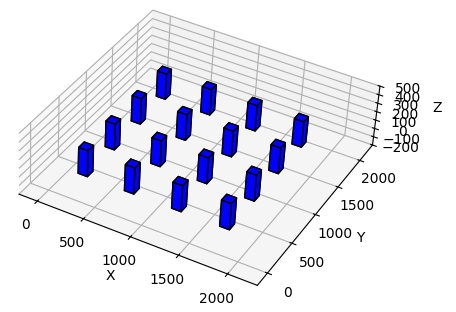
\includegraphics[width=0.65\linewidth]{figs/chap4/Results/4x4/4x4_map.png}
    \caption{4x4 Building Map for 2D algorithm}
    \label{fig:4x4Map}
\end{figure}

\begin{figure}[htbp]
    \centering
    \begin{subfigure}{0.5\textwidth}
        \centering
        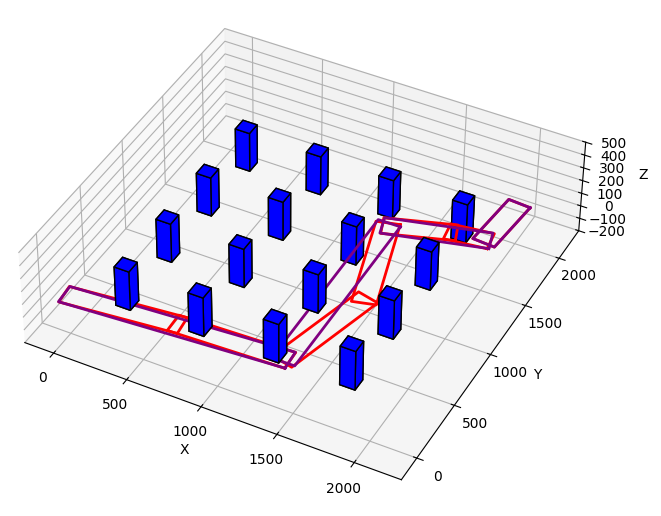
\includegraphics[width=\linewidth]{figs/chap4/Results/4x4/4x4_waypoints.png}
        \caption{Side View of safe flight corridors path through obstacle field.}
        \label{fig:4x4Waypoints1}
    \end{subfigure}
    \hfill
    \begin{subfigure}{0.5\textwidth}
        \centering
        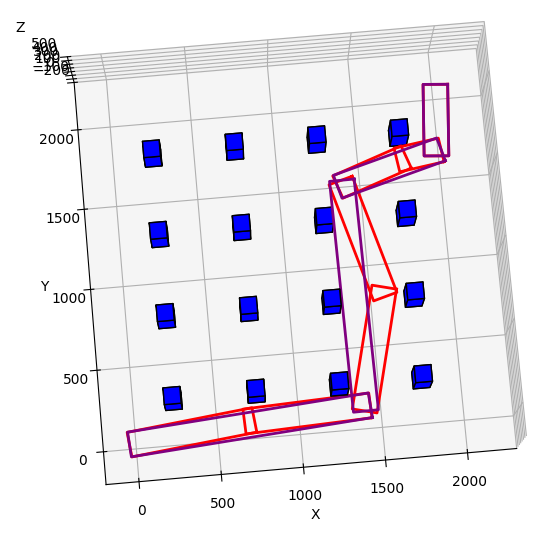
\includegraphics[width=\linewidth]{figs/chap4/Results/4x4/4x4_waypoints_2.png}
        \caption{Top view of same path}
        \label{fig:4x4Waypoints2}
    \end{subfigure}
    
    \caption{Safe flight corridors through obstacle field. The original path is shown in red and the smoothed path is shown in purple.}
    \label{fig:4x4Waypoints}
\end{figure}

\begin{figure}[htbp]
    \centering
    \begin{subfigure}{0.5\textwidth}
        \centering
        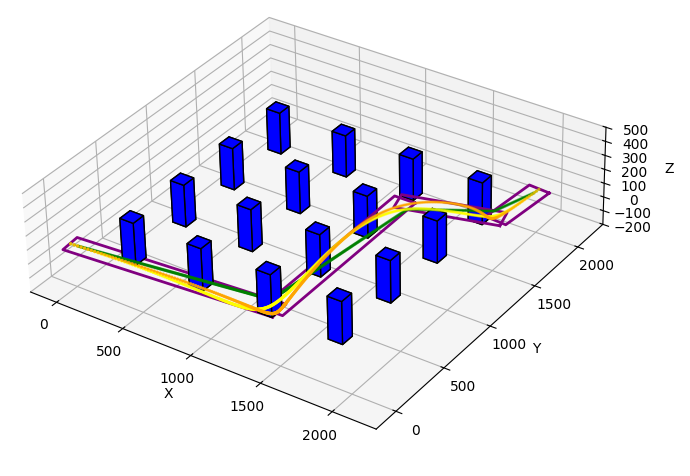
\includegraphics[width=\linewidth]{figs/chap4/Results/4x4/4x4_splines_2.png}
        \caption{Side view of three B-spline paths through SFC path. Green is min distance, yellow is min velocity, orange in min acceleration}
        \label{fig:4x4Splines1}
    \end{subfigure}
    \hfill
    \begin{subfigure}{0.5\textwidth}
        \centering
        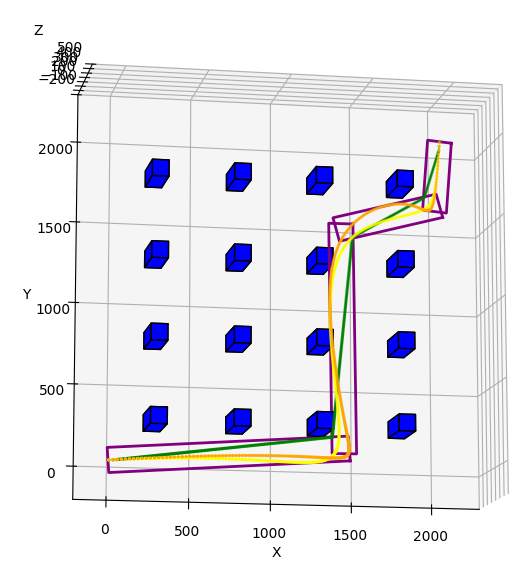
\includegraphics[width=\linewidth]{figs/chap4/Results/4x4/4x4_splines.png}
        \caption{Top view of three B-spline paths through SFC path. Green is min distance, yellow is min velocity, orange in min acceleration}
        \label{fig:4x4Splines2}
    \end{subfigure}
    
    \caption{Spline paths through smoothed SFC path. Path in green generated using minimum distance objective function. Path in yellow generated using minimum velocity objective function. Path in orange generated using minimum acceleration objective function.}
    \label{fig:4x4Splines}
\end{figure}


\begin{figure}
    \centering
    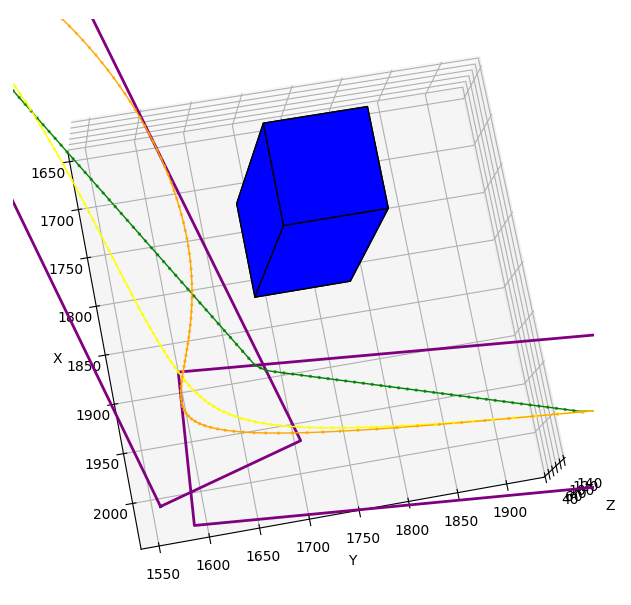
\includegraphics[width=0.9\linewidth]{figs/chap4/Results/4x4/4x4_splines_zoom.png}
    \caption{Zoom in on SFC connection. 
    Comparison of three B-Spline outputs at boundaries. 
    Green is minimum distance, yellow is minimum velocity, and orange is minimum acceleration.}
    \label{fig:4x4Zoom}
\end{figure}

\begin{figure}
    \centering
    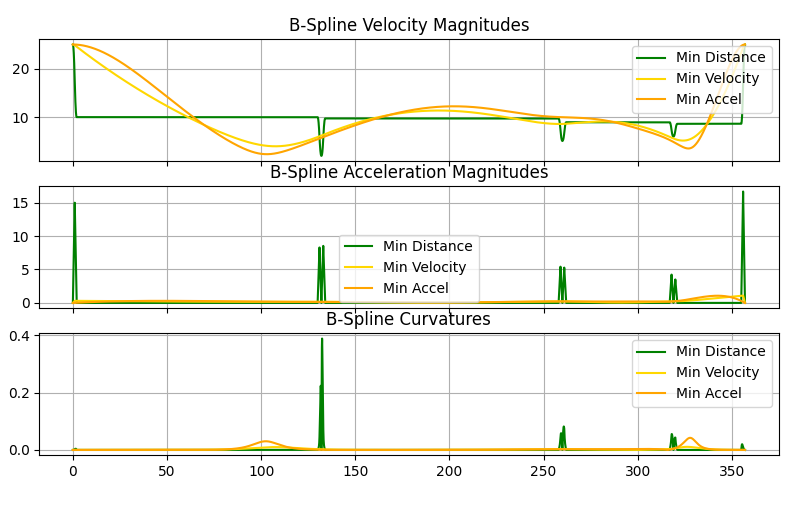
\includegraphics[width=0.9\linewidth]{figs/chap4/Results/4x4/4x4_metrics.png}
    \caption{Metrics from 4x4 test. 
    Comparing results for minimum distance, velocity, and acceleration. 
    Top subplot is velocity for each. Middle subplot is acceleration for each. Bottom subplot is curvature for each.}
    \label{fig:4x4Metrics}
\end{figure}

\subsection{6x6 Grid}

The same experiment was repeated for a 6x6 grid of buildings. 
The size of the area remained the same as before, with a $2000 \times 2000$ meter grid, but the number of obstacles increased from $16$ to $36$. 
The width of the roads were $266$ meters, and the buildings are $66$ meters wide. 
The safe flight corridors remained the same size at $150$ meters. 
The map is a little more cramped, but everything else remained generally the same. 
This algorithm took $18.5$ seconds to run.
Fig. \ref{fig:6x6Map} depicts the $6 \times 6$ building map. 
Fig. \ref{fig:6x6Waypoints} shows the output path map from the RRT algorithm, with both smoothed and unsmoothed SFC paths shown. 
Fig. \ref{fig:6x6Splines} depicts the three B-splines generated within the smoothed flight corridor path. 
Fig. \ref{fig:6x6Zoom} shows a zoomed in section of an intersection.
Fig. \ref{fig:6x6Metrics} shows some metrics for the optimized B-Splines.

\begin{figure}
    \centering
    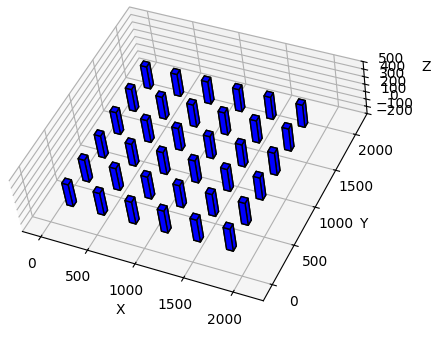
\includegraphics[width=0.65\linewidth]{figs/chap4/Results/6x6/map.png}
    \caption{6x6 Building Map for 2D algorithm}
    \label{fig:6x6Map}
\end{figure}

\begin{figure}[htbp]
    \centering
    \begin{subfigure}{0.45\textwidth}
        \centering
        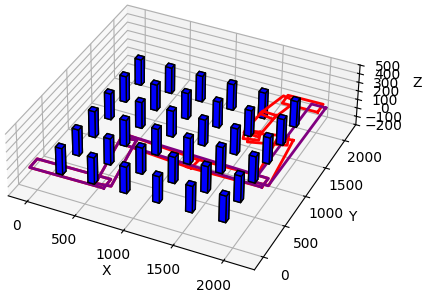
\includegraphics[width=\linewidth]{figs/chap4/Results/6x6/waypoints side.png}
        \caption{Side View of safe flight corridors path through obstacle field.}
        \label{fig:6x6Waypoints1}
    \end{subfigure}
    \hfill
    \begin{subfigure}{0.45\textwidth}
        \centering
        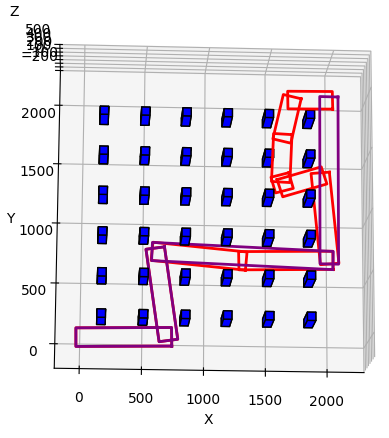
\includegraphics[width=\linewidth]{figs/chap4/Results/6x6/waypoints top.png}
        \caption{Top view of same path}
        \label{fig:6x6Waypoints2}
    \end{subfigure}
    
    \caption{Safe flight corridors through obstacle field. The original path is shown in red and the smoothed path is shown in purple.}
    \label{fig:6x6Waypoints}
\end{figure}

\begin{figure}[htbp]
    \centering
    \begin{subfigure}{0.45\textwidth}
        \centering
        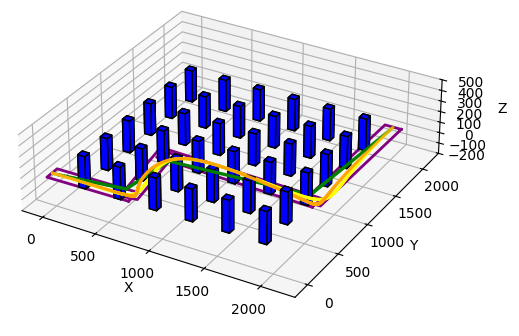
\includegraphics[width=\linewidth]{figs/chap4/Results/6x6/spline side.png}
        \caption{Side view of three B-spline paths through SFC path. Green is min distance, yellow is min velocity, orange in min acceleration}
        \label{fig:6x6Splines1}
    \end{subfigure}
    \hfill
    \begin{subfigure}{0.45\textwidth}
        \centering
        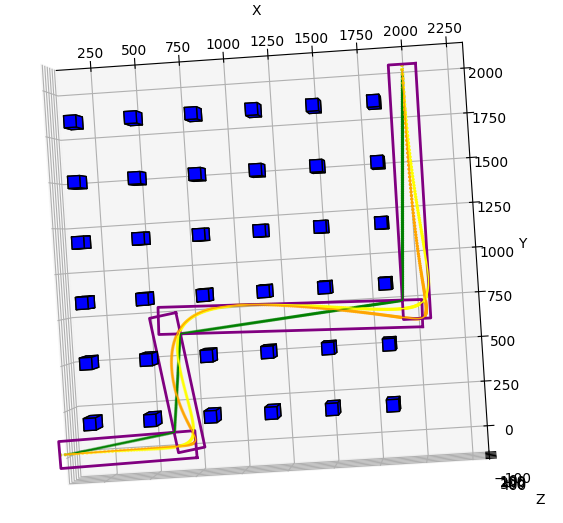
\includegraphics[width=\linewidth]{figs/chap4/Results/6x6/spline top 2.png}
        \caption{Top view of three B-spline paths through SFC path. Green is min distance, yellow is min velocity, orange in min acceleration}
        \label{fig:6x6Splines2}
    \end{subfigure}
    
    \caption{Spline paths through smoothed SFC path. 
             Path in green generated using minimum distance objective function. 
             Path in yellow generated using minimum velocity objective function. 
             Path in orange generated using minimum acceleration objective function.}
    \label{fig:6x6Splines}
\end{figure}

\begin{figure}
    \centering
    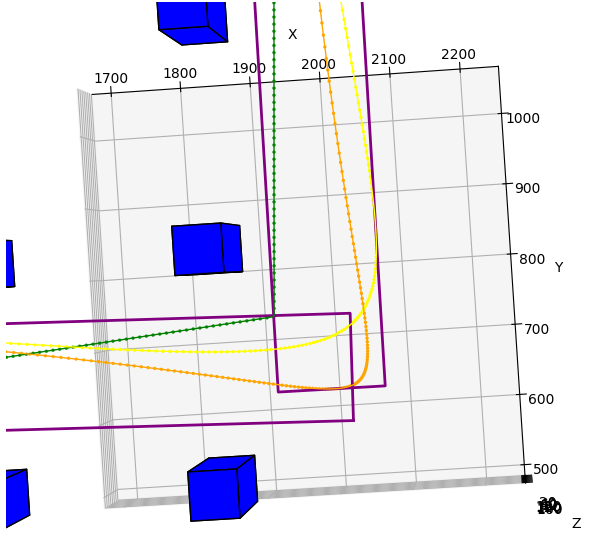
\includegraphics[width=0.9\linewidth]{figs/chap4/Results/6x6/spline top zoom.png}
    \caption{Zoom in on SFC connection. Comparison of three B-Spline outputs at boundaries. Green is minimum distance, yellow is minimum velocity, and orange is minimum acceleration.}
    \label{fig:6x6Zoom}
\end{figure}

\begin{figure}
    \centering
    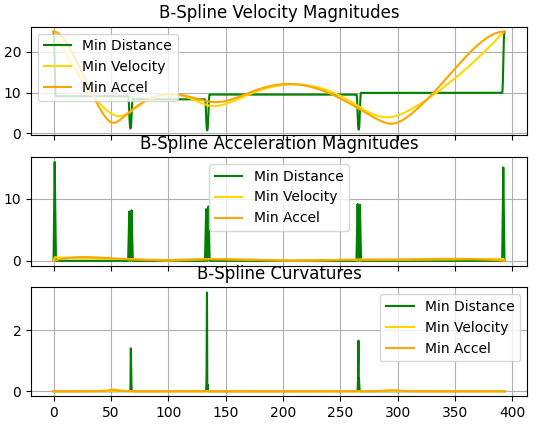
\includegraphics[width=0.9\linewidth]{figs/chap4/Results/6x6/metrics.png}
    \caption{Metrics from 4x4 test. Comparing results for minimum distance, velocity, and acceleration. Top subplot is velocity for each. Middle subplot is acceleration for each. Bottom subplot is curvature for each.}
    \label{fig:6x6Metrics}
\end{figure}


\subsection{Maze}

To demonstrate that the RRT algorithm is capable of generating paths through more confined spaces, a simple maze corridor was created and tested against the algorithm. 
In this case, the RRT algorithm took $19.3$ seconds to run. This took much longer than the building maps, because of the length of this particular maze.
Fig. \ref{fig:MazeMap} depicts the maze map. 
Fig. \ref{fig:MazeWaypoints} shows the output path map from the RRT algorithm, with both smoothed and unsmoothed SFC paths shown. 
Fig. \ref{fig:MazeSplines} depicts the three B-splines generated within the smoothed flight corridor path. 

\begin{figure}
    \centering
    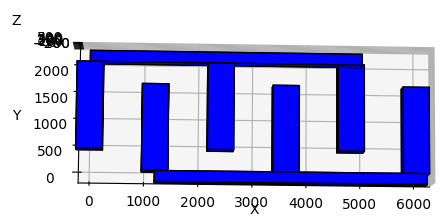
\includegraphics[width=0.65\linewidth]{figs/chap4/Results/Maze/Maze Map.png}
    \caption{Maze Map for 2D algorithm}
    \label{fig:MazeMap}
\end{figure}

\begin{figure}[htbp]
    \centering
    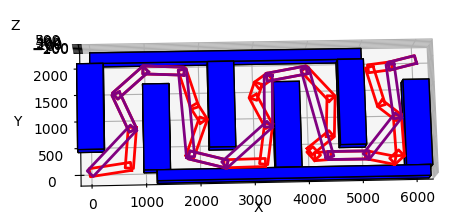
\includegraphics[width=0.65\linewidth]{figs/chap4/Results/Maze/Maze Waypoints.png}
    \caption{Safe flight corridors through maze. The original path is shown in red and the smoothed path is shown in purple.}
    \label{fig:MazeWaypoints}
\end{figure}

\begin{figure}[htbp]
    \centering
    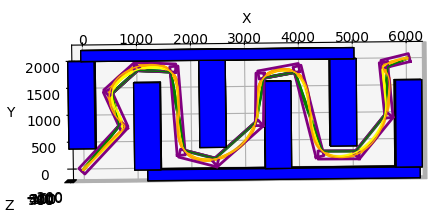
\includegraphics[width=0.65\linewidth]{figs/chap4/Results/Maze/Maze Spline.png}
    \caption{Spline paths through smoothed SFC path. 
             Path in green generated using minimum distance objective function. 
             Path in yellow generated using minimum velocity objective function. 
             Path in orange generated using minimum acceleration objective function.}
    \label{fig:MazeSplines}
\end{figure}

\section{3D RRT Extension}

Naturally, it is desired to not only have 2D paths, but to extend this algorithm to a 3D case with 3D obstacles, 3D safe flight corridors, and 3D B-Spline flight paths. 
This entails creating rectangular prisms for both obstacles and SFCs in the stead of 2D rectangles. 
Instead of searching over an area on a 2D plane, a volume is searched in a 3D space. 
The result is a 3D B-Spline connecting start to finish, which avoids obstacles just as it does in the 2D case.

\subsection{3D Object Definitions}

Each 3D safe flight corridor and obstacle is defined exactly the same as the 2D case using $Ax < b$, but with an added dimension. 
An example of a rectangular prism is shown in Fig. \ref{fig:rectangularPrism}.

\begin{figure}
    \centering
    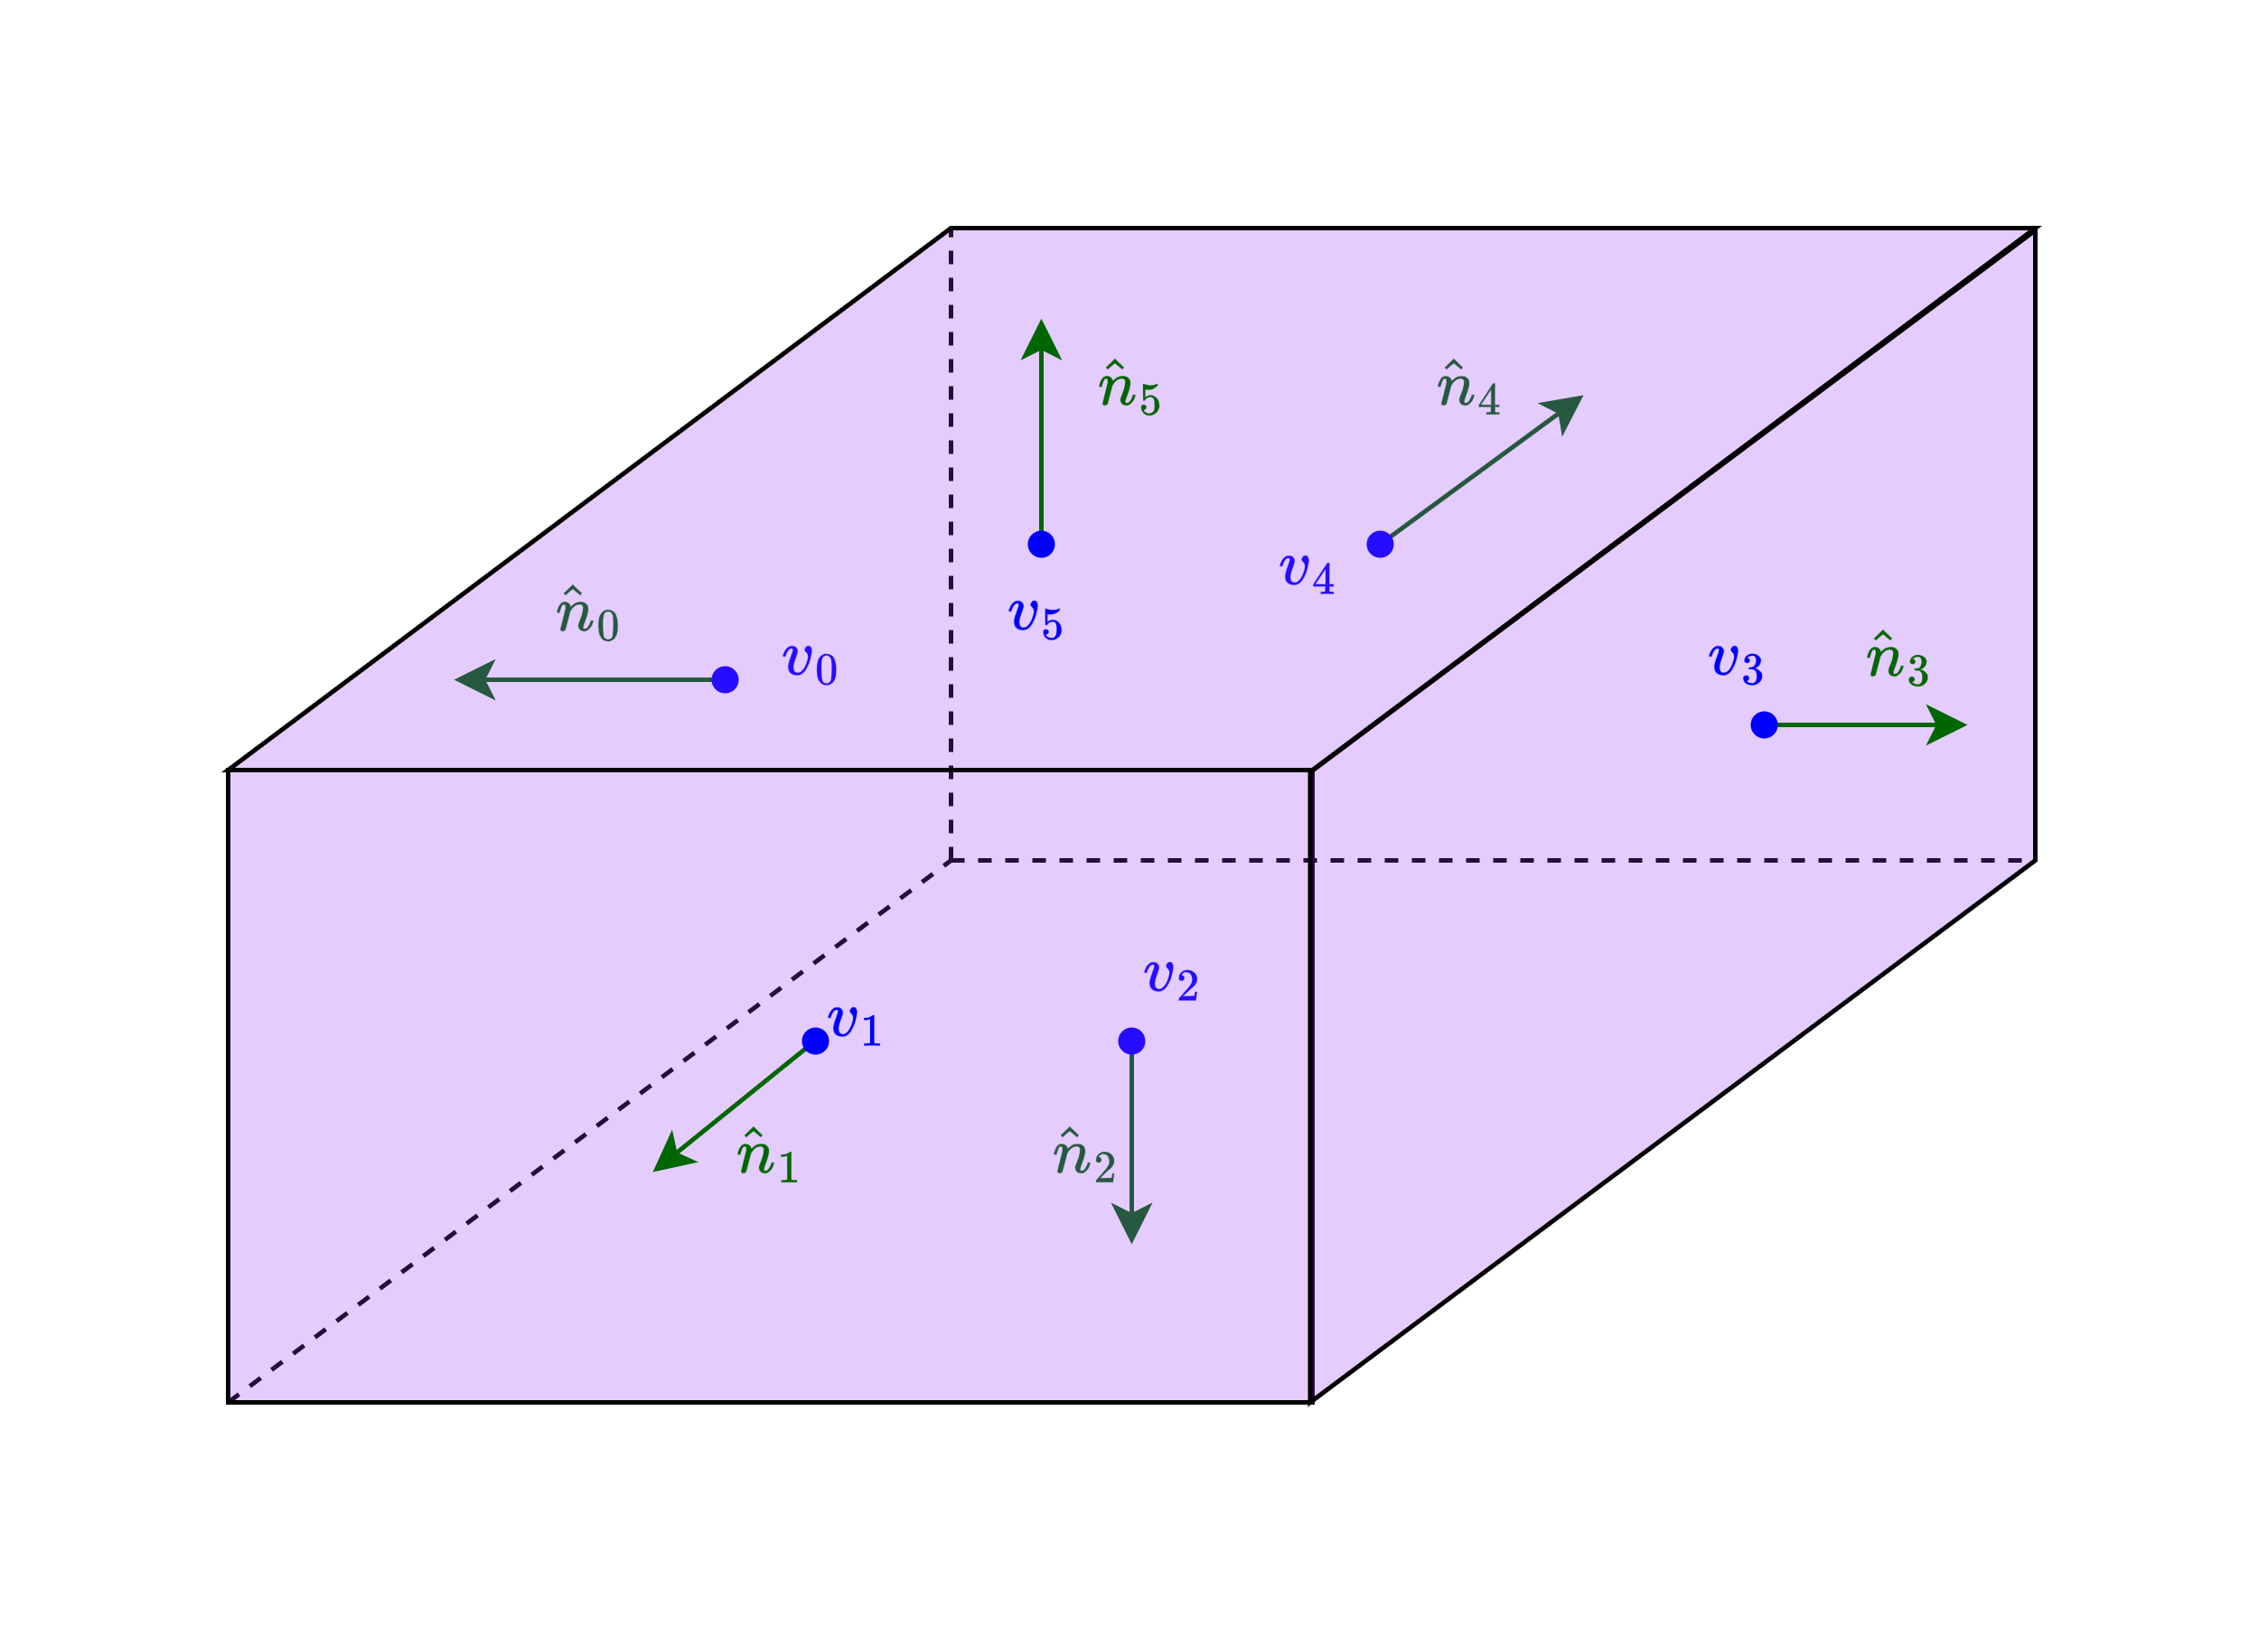
\includegraphics[width=0.5\linewidth]{figs/chap4/Prism Diagram.drawio (2).png}
    \caption{Diagram of a rectangular prism. The normal vectors $n_i$ and sampled points $v_i$ are used to determine whether an object lies within the the prism.}
    \label{fig:rectangularPrism}
\end{figure}

A point $x$ lies within this six-sided rectangular prism if

\begin{align}
    Ax < b \text{, where:}\\
    A = 
    \begin{bmatrix}
        \hat{n}_0^\top\\
        \hat{n}_1^\top\\
        \hat{n}_2^\top\\
        \hat{n}_3^\top\\
        \hat{n}_4^\top\\
        \hat{n}_5^\top\\
    \end{bmatrix}
    \qquad
    b = 
    \begin{bmatrix}
        \hat{n}_0^\top v_0\\
        \hat{n}_1^\top v_1\\
        \hat{n}_2^\top v_2\\
        \hat{n}_3^\top v_3\\
        \hat{n}_4^\top v_4\\
        \hat{n}_5^\top v_5\\
    \end{bmatrix}
\end{align}

is satisfied.

The RRT algorithm follows exactly from the 2D implementation. 
A random point is sampled, connected to the tree, and a rectangular prism drawn around it. 
A 3D safe flight corridor structure is shown in Fig. \ref{fig:3DSafeFlightCorridor}.

\begin{figure}
    \centering
    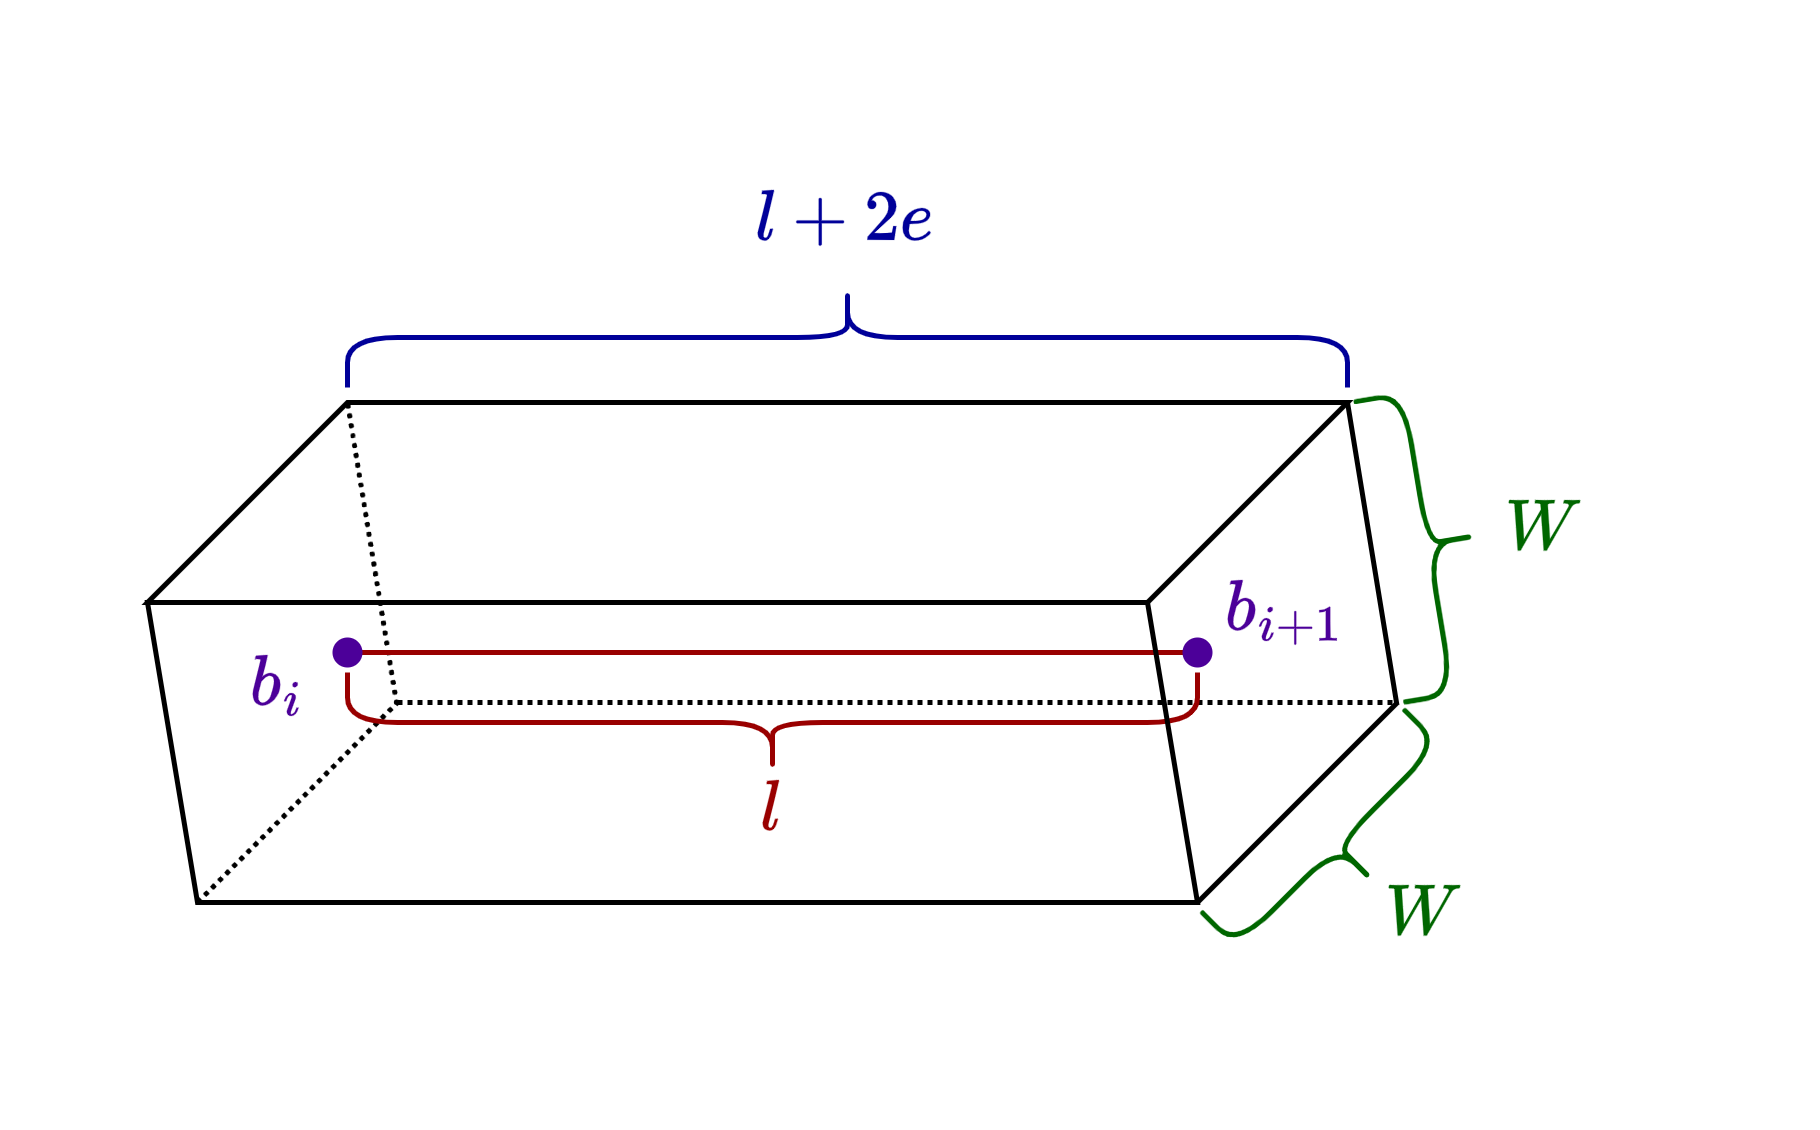
\includegraphics[width=0.5\linewidth]{figs/chap4/3D Safe Flight Corridor.drawio (1).png}
    \caption{Rectangular Prism as a Safe Flight Corridor encompassing points $b_i$ to $b_{i+1}$.}
    \label{fig:3DSafeFlightCorridor}
\end{figure}

\subsection{3D Results}

An experiment was run on a 3D equivalent of the previous 2D experiments. 
A $4 \times 4 \times 4$ obstacle grid was generated on a $2000 \times 2000 \times 2000$ field. 
The obstacles were all uniform cubes of width $150$. 
The initial safe flight corridors were of width $150$, height $150$, and length $700$. 
The start position was $[0.0, 0.0, 0.0]$, and the goal position was $[3000.0, 3000.0, 3000.0]$. 
In one test, RRT algorithm ran in $23.590$ seconds, which is comparable to many 2D algorithm implementations. 
The results are shown in figure \ref{fig:3DRRTResults}.


\begin{figure}[htbp]
    \centering
    \begin{subfigure}{0.48\textwidth}
        \centering
        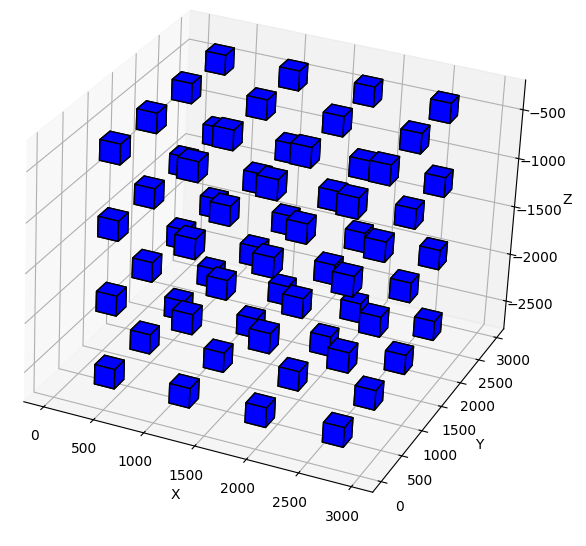
\includegraphics[width=\linewidth]{figs/chap4/Results/3D/map.png}
        \caption{Map of 64 cubical obstacles in $4 \times 4 \times 4$ grid on a $3000 \times 3000 \times 3000$ field. 
                 The object is to find a path from the origin to the opposite diagonal corner.}
        \label{fig:3D_Map}
    \end{subfigure}
    \hfill
    \begin{subfigure}{0.48\textwidth}
        \centering
        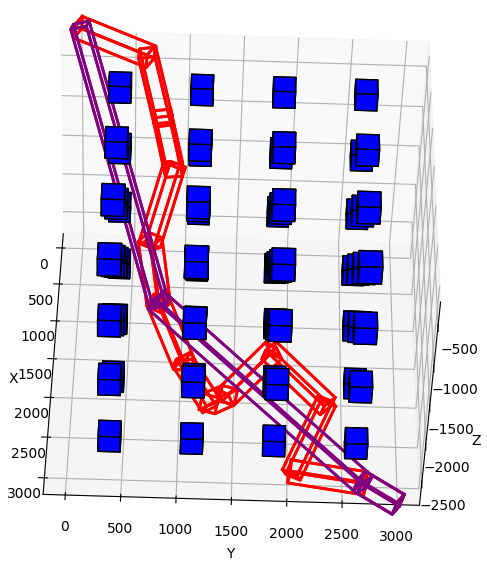
\includegraphics[width=\linewidth]{figs/chap4/Results/3D/waypoints_4.png}
        \caption{Unsmoothed and smoothed SFC paths from start to finish on the same grid. 
                 13 SFCs were initially generated, with 3 SFCs for the smoothed path.}
        \label{fig:3D_waypoints_1}
    \end{subfigure}

    \vspace{0.5cm}  % vertical spacing between rows

    % Row 2
    \begin{subfigure}{0.48\textwidth}
        \centering
        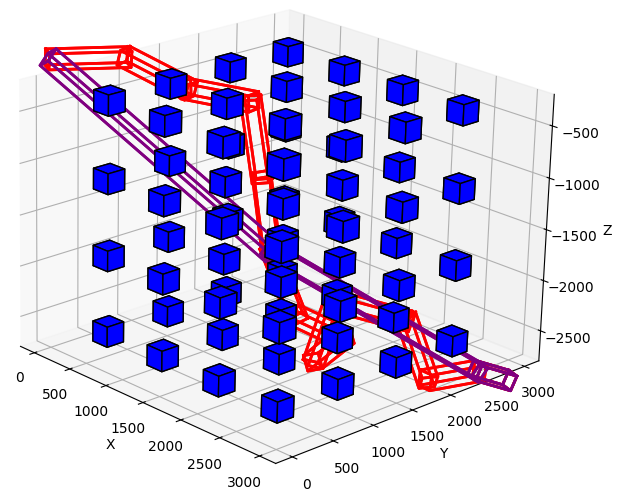
\includegraphics[width=\linewidth]{figs/chap4/Results/3D/waypoints_2.png}
        \caption{Same unsmoothed and smoothed SFC paths from another angle}
        \label{fig:3D_waypoints_2}
    \end{subfigure}
    \hfill
    \begin{subfigure}{0.48\textwidth}
        \centering
        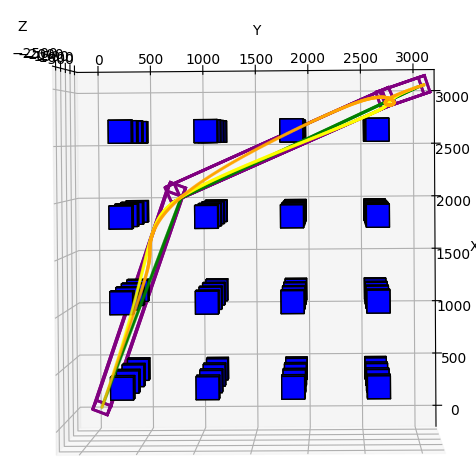
\includegraphics[width=\linewidth]{figs/chap4/Results/3D/splines_5.png}
        \caption{Splines generated through smoothed SFCs}
        \label{fig:3D_Spline}
    \end{subfigure}    
    
    \caption{3D safe flight corridors generated through a $4\times4\times4$ grid of 3D obstacles. 
             The same mathematical principles used in the 2D method were reapplied to 3 dimensional objects.}
    \label{fig:3DRRTResults}
\end{figure}

 A video panning over the exact same safe flight corridors is given at \href{https://youtu.be/WS9w2tG74q0}{3D SFC Pan}, and another video panning over the generated spline path is given at \href{https://youtu.be/n3291vatU08}{3D Spline Pan}. 
 Note that the graphics library Matplotlib used to create these plots does not plot shapes in the correct spatial order. 
 Some of the splines are shown on top of objects that they are actually underneath. 
 This sometimes causes the appearance of an obstacle intersection, even though this is not actually the case.

\section{2D Shapes Within a 3D Environment}

A problem faced in implementing this algorithm was generalizing a 2D path in a 3D environment and generalize it to work with other algorithms. 

It is assumed that all obstacles are 3D convex polyhedra.
This allows the boundaries of an obstacle to take the form of $Ax < b$. 
If it is desired to create a generalized 2D algorithm in a 3D environment, a plane may be specified, and any obstacles intersecting that plane are projected onto it as 2D using the newfound equality constraint, represented as

\begin{align}
    A_2 x = b_2
\end{align}

or equivalently

\begin{align}
    ax + by + cz = d
\end{align}.


\begin{align}
    \Vec{p}(t) =
    \begin{bmatrix}
        x(t)\\
        y(t)\\
        z(t)\\
    \end{bmatrix}
\end{align}

\begin{align*}
    \hat{n}, p_0\\
    Q = \text{null}\{\hat{n}\}\\
    y \in \mathbb{R}^2, x \in \mathbb{R}^3\\
    x = p_0 + Qy\\
    AQy < b - Ap_0
\end{align*}

Using the Moore-Penrose Pseudoinverse, we can find the 2D representation of a 3D vector which already lies on the plane. 
Because $Q$ is a tall, full rank matrix $(3 \times 2)$, a left pseudoinverse of the form $Q^+ = (Q^\top Q)Q^\top$ will get the best solution for $y$ as

\begin{align*}
    y = Q^+ (x-p_0)\\
    Q^+ = (Q^\top Q)Q^\top\\
\end{align*}.

The method of obtaining an orthonormal basis $Q$ from a normal vector $\hat{n}$ is described in section \ref{sec:2DProjection}.

\section{Future Work}

Several areas of this algorithm stand to be improved in the future. 
Future research in this area must draw upon other related works. 
For example, \cite{SUN2025103174} describes a similar algorithm that generates adaptive safe flight corridors that morph into the empty area between obstacles, while maintaining minimum turning radius constraints. 
Also, in \cite{osburn} a method of generating time varying Bezier splines through a time-varying obstacle field using convex safe regions.
Some of the current limitations and possible solutions are presented.

\subsection{Dijkstra's Algorithm and Turn Constraints}

One limitation is Dijkstra's Algorithm and turning constraints. 
The algorithm generates a minimum distance path given a set of initial guesses, called the unsmoothed waypoints, and generates the shortest distance path from start to finish. 
However, there is no guarantee on a shortest distance path that satisfies angular constraints, or the angle between two safe flight corridors. 

One can imagine a scenario where the algorithm paints itself into a corner. 
The shortest found path may find an optimal path up to a node, where none of the new segments violate the turn constraint. 
The addition of a new segment may yet violate the turn constraint with all possible forward node connections.
Thus, the algorithm can be broken, as illustrated in Fig. \ref{fig:DijkstraScenario}. 
In this diagram, a setup of $5$ waypoints is shown with $4$ segments connecting those $5$ nodes. 
In the primary algorithm, nodes were only added to the tree if they satisfied the turning constraint. 
In this case, each segment angle must be greater than $120^{\circ}$. 
The algorithm also finds that there are $2$ other segments that satisfy the intersection constraint, but not necessarily the angular constraint. 


\begin{figure}
    \centering
    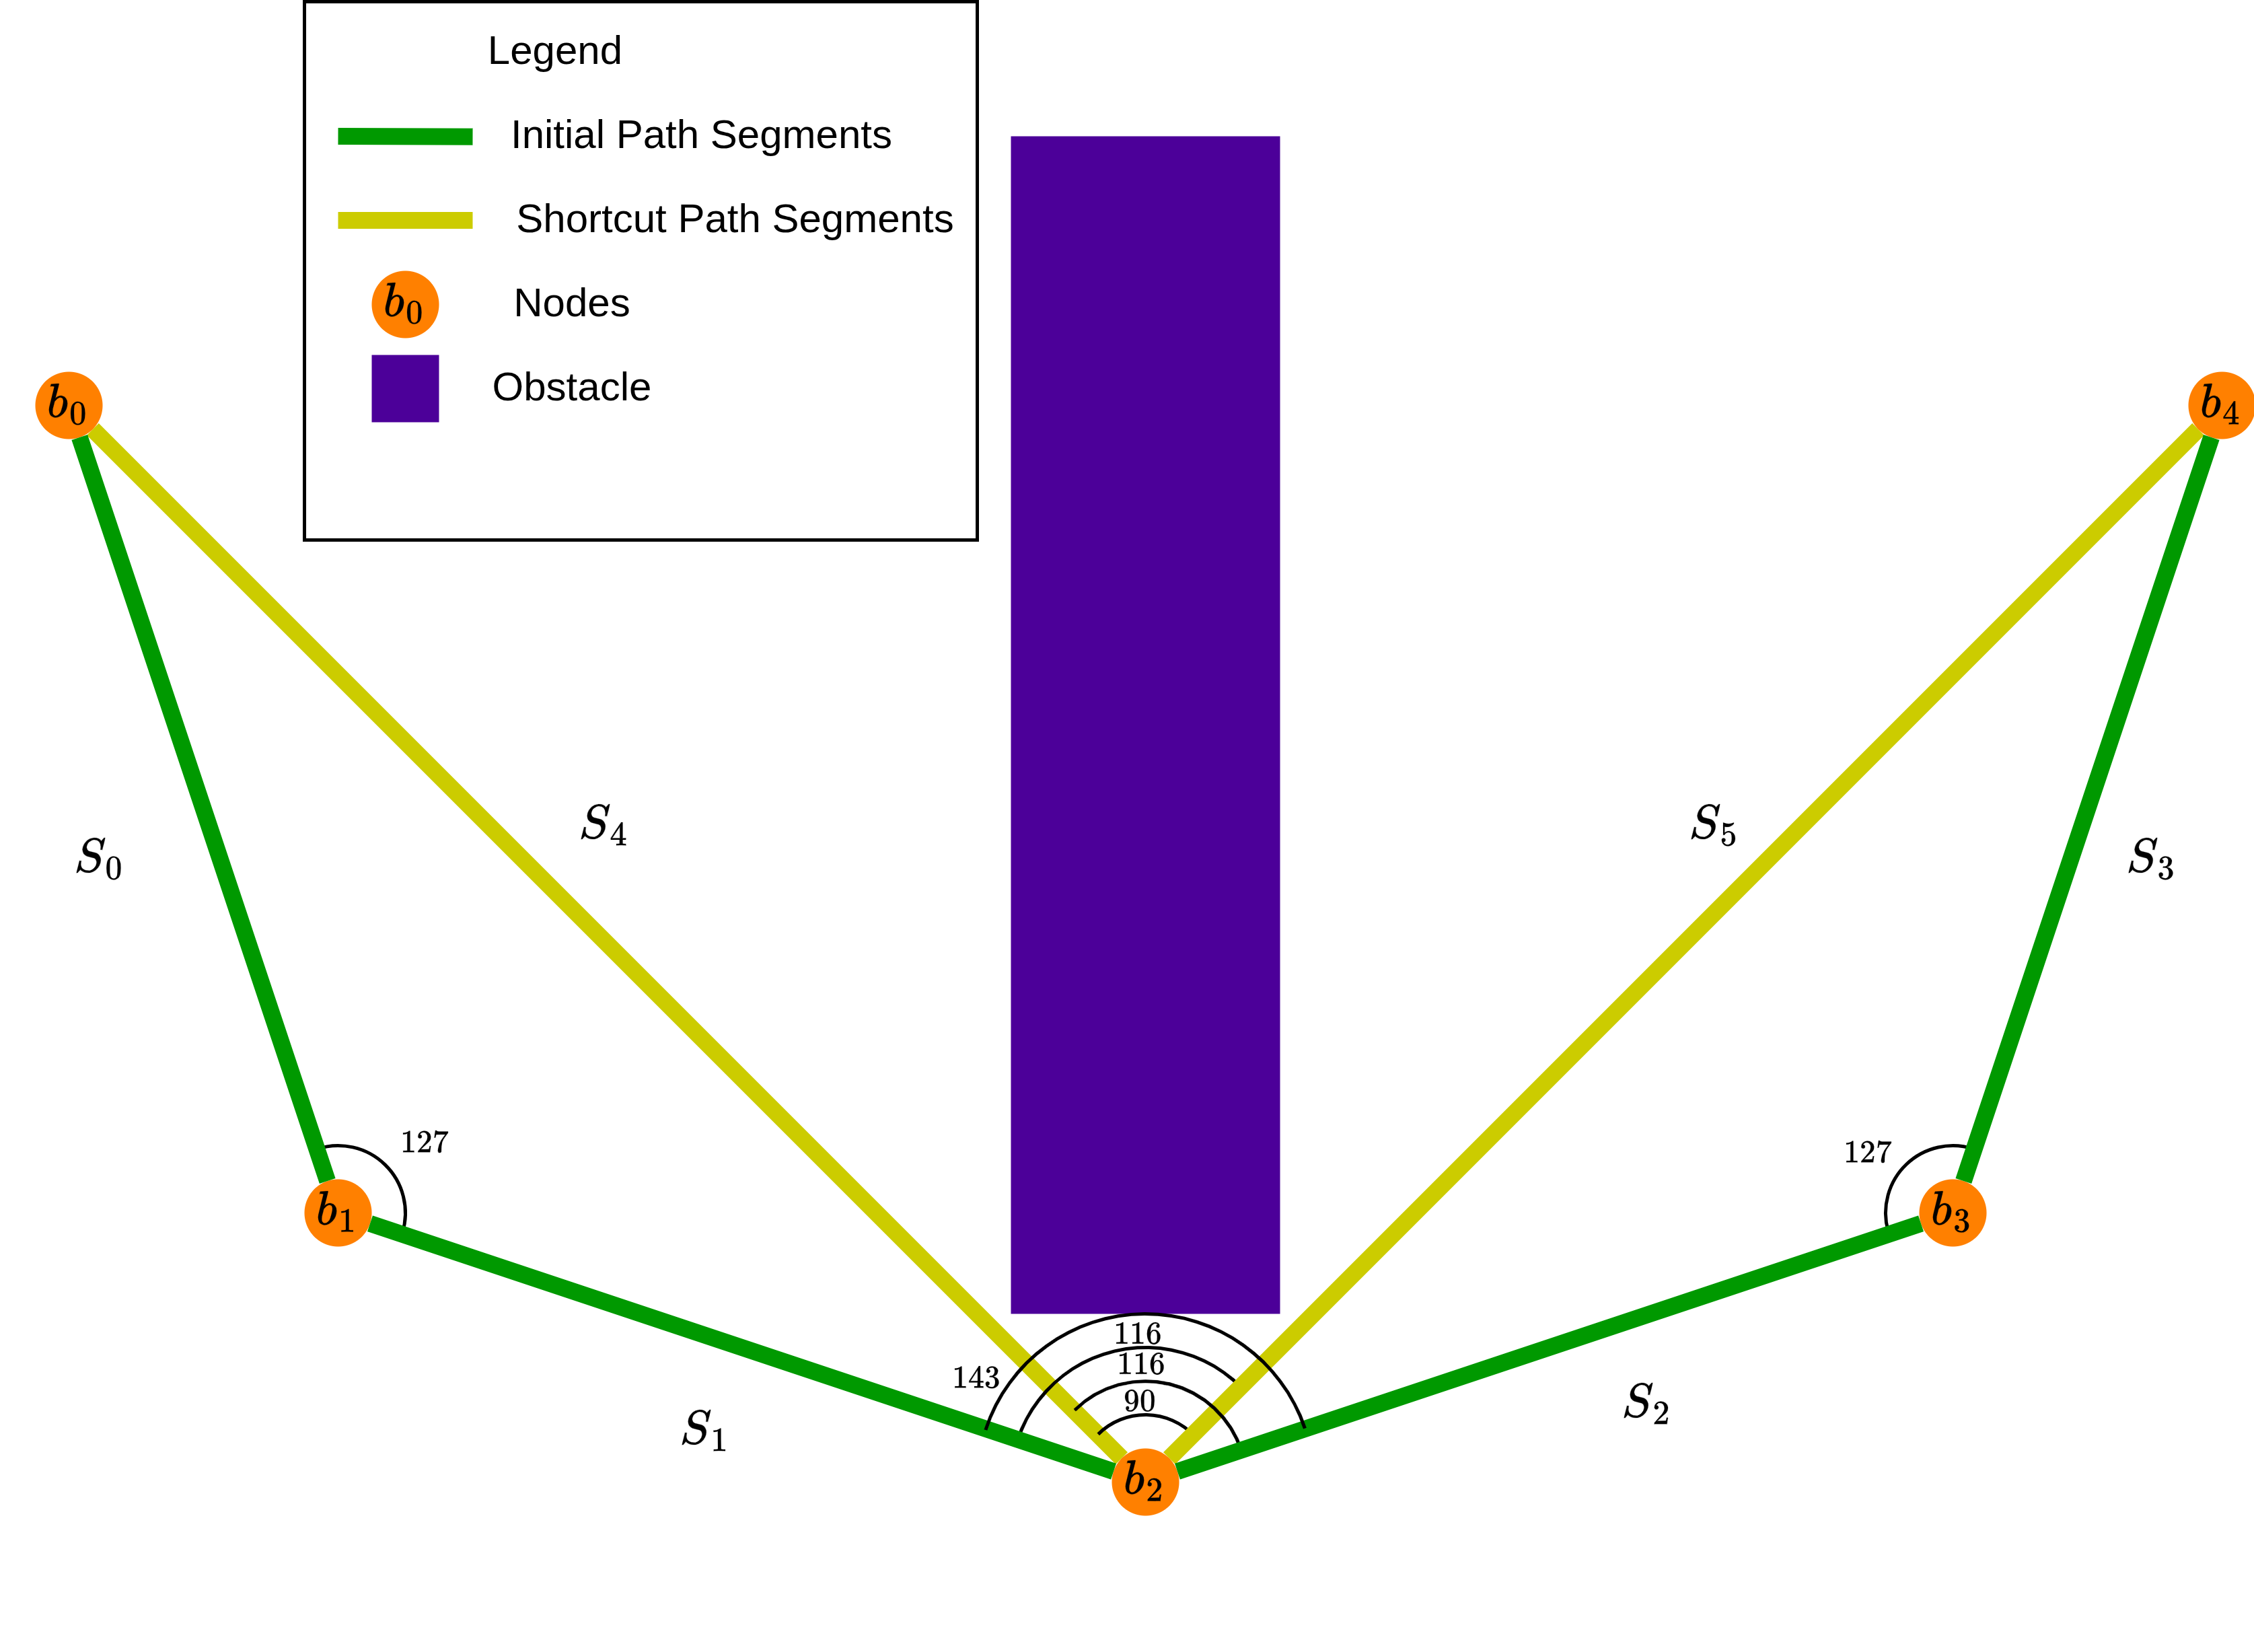
\includegraphics[width=0.8\linewidth]{figs/chap4/Turn Rate Constraints/Dijkstras Scenario.drawio.png}
    \caption{Example setup of waypoints which Dijkstra's Algorithm would be utilized to smooth. Angles between each segment are given.}
    \label{fig:DijkstraScenario}
\end{figure}

The problem with Dijkstra's algorithm is that it will select segment $S_4$ to connect $b_0$ and $b_2$ and bypass $b_1$, where we assume that adding $S_4$ does not violate angular constraints with the previous line segment not shown in this diagram for simplicity. 
Now that the algorithm is at $b_2$, it has to choose between $S_2$ and $S_5$. 
Unfortunately, both choices violate the minimum turn constraint with $90^{\circ}$ and $116^{\circ}$, respectively, which causing the algorithm to fail. 
This is illustrated in Fig. \ref{fig:DijkstraDilemma}.

\begin{figure}
    \centering
    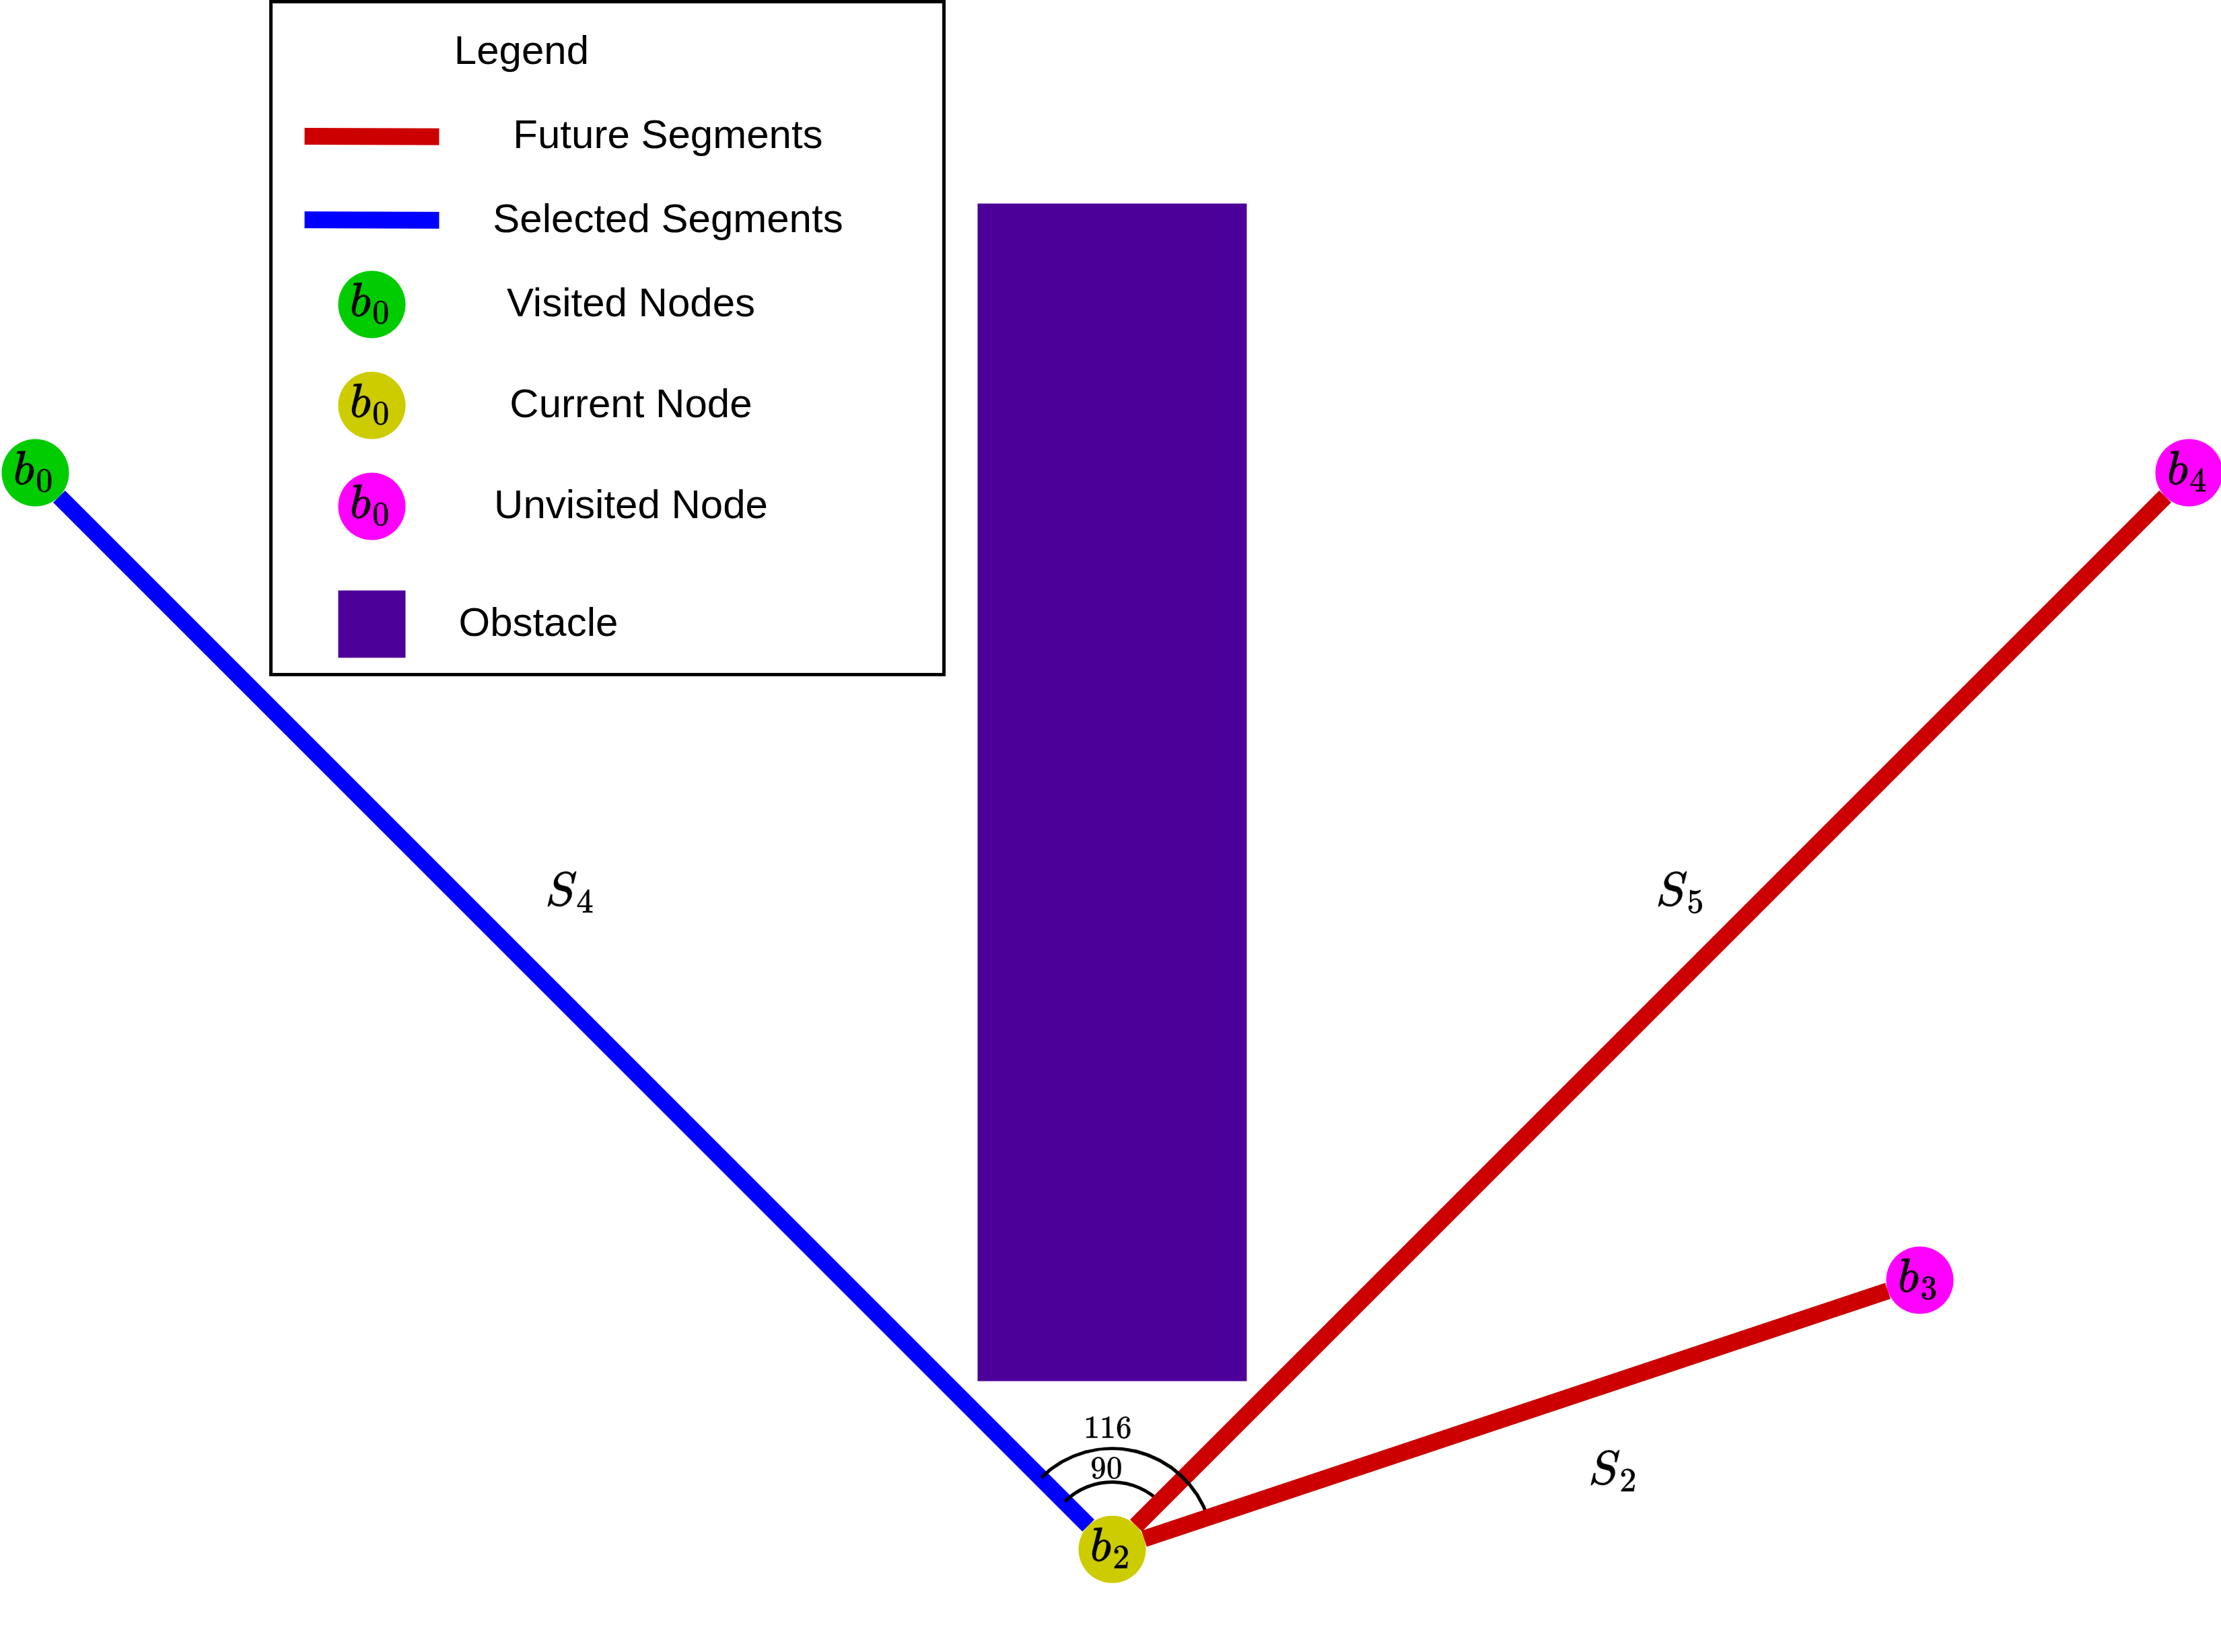
\includegraphics[width=0.8\linewidth]{figs/chap4/Turn Rate Constraints/Dijstras Dilemma.drawio.png}
    \caption{Dilemma of Dijkstra's algorithm with angular constraint at $b_2$}
    \label{fig:DijkstraDilemma}
\end{figure}

Solving this problem is beyond the scope of this thesis, but it does pose an interesting problem for future research. 
The best solution that has been found is an algorithm called LIAN, along with its many derivatives. 
LIAN is derived from the term "Limited Angle", so it is a limited angle path algorithm. 
LIAN was introduced in 2015 in \cite{LIAN} as a variant of $A^*$. 
LIAN works by storing two copies of each node and working backward if the angle constraint is ever violated. 
In \cite{LIAN}, success rates in the high $90$ percentages were achieved. 
Another paper was published in 2018 on eLIAM or enhanced LIAM that solved an angle-constrained problem 20\% more often than standard LIAM. 
Implementation of LIAM, or some other algorithm, will generate a more robust framework for a better algorithm.

\subsection{Turn Constraints}

It is demonstrated in section \ref{sec:Turn Constraints} how to find the maximum angle between two SFCs given a minimum turning radius constraint. 
In the previous section, the necessity for an SFC smoothing algorithm that maintains angular conditions was discussed. 
However, a resulting B-Spline within the annulus does not automatically conform to the minimum turning radius constraint. 
Even with segmented annulus constraints along each SFC intersection. 
There is no guarantee that the control points will remain along the inside turning radius. 
Many edge cases exist that violate the minimum turning radius. 

Curvature measures how sharply a function turns. 
The tighter the turn on a particular curve, the higher the curvature. 
It is defined as $\frac{1}{R}$, where $R$ is the radius of the circle tangential to the curve. 
This is shown in figure \ref{fig:curvature}. 

\begin{figure}
    \centering
    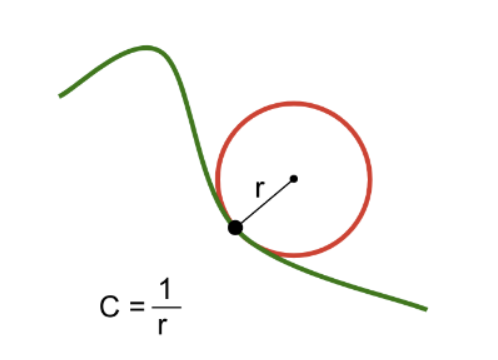
\includegraphics[width=0.5\linewidth]{figs/chap4/Curvature.png}
    \caption{Tangential circle radius and curvature. Reproduced from \cite{david_bspline}}
    \label{fig:curvature}
\end{figure}

The definition for curvature of a B-Spline $C(t)$ is

\begin{align}
    C(t) = \frac{|| \dot{b}(t) \times \ddot{b}(t)||}{||\dot{b}(t)||^3}
\end{align}.

Notice that this formula does not directly involve the control points, but only includes the actual B-Spline equation. 
This makes it difficult to directly minimize curvature of a B-Spline generated within a safe flight corridor.

Curvature constraints on B-Splines is an open area of research which extends beyond the scope of this paper. 
Several tools are being developed to minimize high curvature in B-Splines including the use of neural networks. 
For example, Deep Learning Parametrization for B-Spline Curve Approximation \cite{laube2018deeplearningparametrizationbspline} describes using neural networks to modify the knot vector of a B-Spline to minimize sections of high curvature. 
However, this particular paper works with obstacle avoidance, and not safe flight corridors. 
A future research project would involve the same RRT and smoothing algorithms, and would modify the positions of the control points via a neural network, while maintaining the current SFC constraints. 

\subsection{Real Time Implementation}

This paper has assumed that all obstacle fields are static and predetermined. 
There are no moving obstacles in the environment, and the entire environment is known in its entirety before path generation takes place. 
In practice, these assumptions may not always hold. 
We may want to generate paths through an environment with moving obstacles, such as a construction site. 
The UAV may be dynamically mapping its environment with lidar or ultrasonics, so not all obstacles may be know beforehand. 

In both of these cases, a fast algorithm is needed that can quickly rerun the RRT algorithm based on newly acquired information. 
Unfortunately, the present algorithm is too slow for such use. 
For example, during a test on the $6\times6$ grid, the RRT generation segment took $38.58$ seconds, and the cumulative time to generate the three control point paths was $7.27$ seconds, which is obviously far too slow. 
Real time implementation will require the total algorithm run time to be ideally less than one second.

Several possible solutions exist which may help reduce computation time. 
First, this entire algorithm is written in Python; rewriting many of the computationally intensive functions in a faster language such as C or Rust may help significantly. 
Currently, the algorithm checks every obstacle in the field for intersection.
An obstacle reduction algorithm may be written that only checks for obstacles in the direct vicinity of the SFC, which may decrease the computation time. 
The RRT algorithm is currently entirely random, with no biasing towards the end goal. 
Biased RRT sampling, which was introduced in \cite{Urmson_2003_8792}, and the greedy RRT algorithm, introduced in \cite{LaValle_greedy}, may help this as well. 
A relatively new paper \cite{Gammell-2014-7921} introduces an informed RRT algorithm that maintains the same convergence probability of the original algorithm, while also significantly reducing computational time. 

\subsection{3D limitations}

The largest bottleneck in the 2D algorithm is the RRT searching period, which is exacerbated by the increased complexity of searching with rectangles instead of traditional lines. 
This problem becomes even more exacerbated in the 3D algorithm. 
The number of samples required to generate a path is proportional to $length^3$ instead of $length^2$ for the 2D case, as does the number of obstacles to check against. 
Also, each obstacle and SFC has 6 3D constraints instead of 4 2D constraints, which means more variables need to be checked for feasibility. 
The complexity of the 3D case must be reduced in order for a viable real time 3D implementation to work.

\subsection{Annulus Constraints}

The current implementation of annulus constraints is also in its infancy. 
Numerous issues exist in the present implementation. 
For example, the annulus segments of one SFC intersection may sometimes intersect with the annulus segments of the next SFC intersection. 
Such intersections may lead to infeasible constraints on the control points and cause the control point optimizer to fail. 
An example of this is shown in figure \ref{fig:annulusOverlap}. 
Future work in this area will have to take into account all such edge cases of these annulus constraints.

\begin{figure}
    \centering
    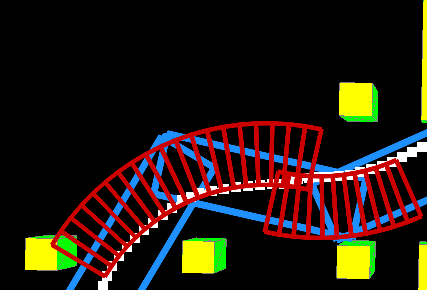
\includegraphics[width=0.5\linewidth]{figs/chap4/annulus/complete path expanded wall zoom.png}
    \caption{Example of overlapping annulus constraints between two safe flight corridor corners. Such overlapping may cause infeasible constraints on B-Spline generation.}
    \label{fig:annulusOverlap}
\end{figure}

Currently, there are no 3D annulus constraints on the 3D Waypoint implementation. 
Developing a more robust constraint framework and developing a 3D implementation of this would be a strong foundation for a future paper on this subject.

\section{Conclusion}

The field of controls and robotics is becoming saturated with control problems. 
As unmanned aircraft become more prevalent, there is an increased need for path planning algorithms. 
Such algorithms that can also avoid obstacles are especially important for applications in the field. 
B-Splines are a growing area of research for flight paths because of their ability to be parameterized by control and knot points. 
The solution presented in this section is a path planning algorithm that avoids obstacles.
It is a variation of the RRT algorithm that uses safe flight corridors instead of straight lines.
Within those SFCs, a B-Spline path is generated.
This work may add another tool in the development of obstacle avoiding algorithms.
